%% Template para dissertacao/tese na classe UFBAthesis
%% versao 1.0
%% (c) 2005 Paulo G. S. Fonseca
%% (c) 2012 Antonio Terceiro
%% (c) 2014 Christina von Flach
%% www.dcc.ufba.br/~flach/ufbathesis

%% Carrega a classe ufbathesis
%% Opcoes: * Idiomas
%%           pt   - portugues (padrao)
%%           en   - ingles
%%         * Tipo do Texto
%%           bsc  - para monografias de graduacao
%%           msc  - para dissertacoes de mestrado (padrao)
%%           qual - exame de qualificacao de mestrado
%%           prop - exame de qualificacao de doutorado
%%           phd  - para teses de doutorado
%%         * Media
%%           scr  - para versao eletronica (PDF) / consulte o guia do usuario
%%         * Estilo
%%           classic - estilo original a la TAOCP (deprecated) - apesar de deprecated, manter esse.
%%           std     - novo estilo a la CUP (padrao)
%%         * Paginacao
%%           oneside - para impressao em face unica
%%           twoside - para impressao em frente e verso (padrao)

% Atenção: Manter 'classic' na declaracao abaixo:
\documentclass[qual, classic, a4paper]{ufbathesis}

%% Preambulo:
\usepackage[utf8]{inputenc}

%\usepackage[authoryear]{natbib}
\usepackage{graphicx}
\usepackage{lipsum}
\usepackage{hyphenat}
\usepackage[usenames, dvipsnames, table]{xcolor}
\usepackage{booktabs}
\usepackage{pifont}
\usepackage{multirow}
\usepackage{listings} 
\usepackage{colortbl}
\usepackage{xfrac}
\usepackage[FIGTOPCAP]{subfigure}
\usepackage{tabularx}
\usepackage{ragged2e}
\usepackage{acronym}
\usepackage{float}
\usepackage{todonotes}
\usepackage{amssymb}
\usepackage{placeins}
\usepackage{arydshln}

\presetkeys%
    {todonotes}%
    {inline,backgroundcolor=yellow}{}
    
\usepackage{blindtext}

\usepackage{tikz}
\usetikzlibrary{arrows,shapes,positioning,shadows,trees}

% Siglas
\acrodef{AM}[AM]{{Aprendizado de Máquina}}
\acrodef{DE}[DE] {{Distância Euclidiana}}
\acrodef{FCD}[FCD] {{\textit {Fluxo de Dados Contínuos}}}
\acrodef{DN}[DN] {{\textit {Detecção de Novidade}}}

% Universidade
\university{Universidade Federal da Bahia}

% Endereco (cidade)
\address{Salvador}

% Instituto ou Centro Academico
\institute{Instituto de Matem\'{a}tica}

% Nome da biblioteca - usado na ficha catalografica
\library{Biblioteca Reitor Mac\^{e}do Costa}

% Programa de pos-graduacao
\program{Programa de P\'{o}s-Gradua\c{c}\~{a}o em Ci\^{e}ncia da Computa\c{c}\~{a}o}

% Area de titulacao
\majorfield{Ci\^{e}ncia da Computa\c{c}\~{a}o}

% Titulo da dissertacao
\title{Aplicando redes de função de base radial para detecção de mudanças de conceito em fluxos contínuos de dados}

% Data da defesa
% e.g. \date{19 de fevereiro de 2013}
\date{03 de Abril de 2019}
% e.g. \defenseyear{2013}
\defenseyear{2019}

% Autor
% e.g. \author{Jose da Silva}
\author{Ruivaldo Azevedo Lobão Neto}

% Orientador(a)
% Opcao: [f] - para orientador do sexo feminino
% e.g. \adviser[f]{Profa. Dra. Maria Santos}
\adviser{Ricardo Ara\'{u}jo Rios}

% Orientador(a)
% Opcao: [f] - para orientador do sexo feminino
% e.g. \coadviser{Prof. Dr. Pedro Pedreira}
% Comente se nao ha co-orientador
%\coadviser{Nome Completo do CO-ORIENTADOR}

%% Inicio do documento
\begin{document}

\pgcompfrontpage

%% Parte pre-textual
\frontmatter

\pgcomppresentationpage

%%%%%%%%%%%%%%%%%%%%%%%%%
% Ficha catalografica
%%%%%%%%%%%%%%%%%%%%%%%%%

%\authorcitationname{Silva, Mirlei Moura da } % e.g. Terceiro, Antonio Soares de Azevedo
%\advisercitationname{Sobrenome, Nome do ORIENTADOR} % e.g. Chavez, Christina von Flach Garcia
%\coadvisercitationname{Sobrenome, Nome do CO-ORIENTADOR} % e.g. Mendonca, Manoel Gomes de
%\catalogtype{Disserta\c{c}\~{a}o (Mestrado)} % e.g. ou ``Tese (Doutorado)''

%\catalogtopics{1. Primeira palavra-chave. 2. Segunda palavra-chave. 3. Terceira palavra-chave} % Listar palavras-chave do trabalho para a FICHA CATALOGRAFICA}, por exemplo, ``1. Complexidade Estrutural. 2. Qualidade de Software 3. Engenharia de Software''
%\catalogcdd{XXX.XX} % e.g.  XXX.XX (número nesse formato serah dado pela biblioteca)
%\catalogcdu{XXX.XX.XXX} % e.g.  XXX.XX.XXX (idem) 
%\catalogingsheet

%%%%%%%%%%%%%%%%%%%%%
% Termo de aprovacaoo
%%%%%%%%%%%%%%%%%%%%%

\approvalsheet{Salvador, 03 de Abril de 2019}{
   \comittemember{Prof. Dr. Ricardo Araújo Rios}{UFBA}  
   %\comittemember{Profa. Dr...}{UFBA}
   %\comittemember{Prof. Dr...}{USP} 
}
   % Para mestrado, apenas 3.
   % \comittemember{Prof. Dr. Professor 4}{Universidade HJKL}
   % \comittemember{Profa. Dra. Professora 5}{Universidade QWERTY}

%%%%%%%%%%%%%%%%%%%%%%%%%%%%%%%%%%%%%%%% 
% Dedicatoria, Agradecimentos, Epigrafe
%%%%%%%%%%%%%%%%%%%%%%%%%%%%%%%%%%%%%%%%

% Comente para ocultar
%\begin{dedicatory}
%DIGITE A DEDICATORIA AQUI
%\end{dedicatory}

% Agradecimentos
% Se preferir, crie um arquivo `a parte e o inclua via \include{}
%\acknowledgements
%DIGITE OS AGRADECIMENTOS AQUI

% Epigrafe
%\begin{epigraph}[NOTA]{AUTOR}
%DIGITE AQUI A CITACAO
%\end{epigraph}

%%%%%%%%%%%%%%%%%%%%%
% Resumo 
%%%%%%%%%%%%%%%%%%%%%
\resumo

\blindtext

% Palavras-chave do resumo em Portugues
\begin{keywords}
    Aprendizado de Máquina, Fluxos Contínuos de Dados, Mudanças de Conceito, Redes de Função de Base Radial, Não supervisionado
\end{keywords}

\abstract

\blindtext

% Palavras-chave do resumo em Ingles
\begin{keywords}
    Machine Learning, Data Streams, Concept Drift, Radial Basis Function Networks, RBF Network, Unlabeled
\end{keywords}

%%%%%%%%%%%%%%%%%%%
% Sumario / Indice
%%%%%%%%%%%%%%%%%%%

% Comente para ocultar
\tableofcontents

% Lista de figuras
% Comente para ocultar
\listoffigures

% Lista de tabelas
% Comente para ocultar
\listoftables

%% Parte textual
\mainmatter

% Eh aconselhavel criar cada capitulo em um arquivo separado, digamos
% "capitulo1.tex", "capitulo2.tex", ... "capituloN.tex" e depois
% inclui-los com:
% \include{capitulo1}
% \include{capitulo2}
% ...
% \include{capituloN}
%
% Importante: 
% Use \xchapter{}{} ao inves de \chapter{}; se não quiser colocar texto antes do inicio do capitulo, use \xchapter{texto}{}.

%%%
\xchapter{Introdução}{} \label{introducao}

\section{Contexto e Motivação}

A quantidade de dados produzidos por sistemas computacionais tem crescido exponencialmente nos últimos anos.
Relatório produzido pelo IDC (\textit{International Data Corporation}), estimava que em 2014 seriam produzidos 4,4 zettabytes (trilhões de gigabytes) de dados \cite{idc_report}.
O mesmo relatório, projeta que em 2019 essa quantidade será de 44 zettabytes.

Parte significativa dessas informações é criada atráves de Fluxos Contínuos de Dados (FCDs).
Estes fluxos caracterizam-se por produzirem novos eventos de forma contínua, ordenada, em alta frequência e potencialmente infinita \cite{Feigenbaum:2003:ALD:589343.592594}.
Diversos domínios de aplicação atuam dessa forma, incluindo:
monitoramento de sensores \cite{Lee:Wang:Ryu:2007},
tráfico TCP/IP, 
histórico de compra de clientes,
filtragem de SPAM em mensagens de e-mail \cite{Katakis:2010:TRC:1746286.1746291},
detecção de intrusos,
análise de sentimentos \cite{Smailovic:2014:SAL:2941772.2941857}, 
etc.

Diante desse cenário, a adaptação de técnicas de Aprendizado de Máquina (AM) para contextos com FCDs tem se tornado uma importante e desafiadora área de pesquisa.
Isto ocorre, pois, nestas circustâncias os algoritmos de AM devem atender a severas restrições de tempo e processamento \cite{Bifet:2009:ALM:1656274.1656287}.

Além disso, a maioria das aplicações reais que envolvem FCDs são dinâmicas.
Isto é, ao longo do tempo, o contexto implícito do processo gerador ou a distribuição dos dados produzidos podem sofrer alterações, modificando os conceitos-alvo esperados.
Na literatura, este problema é denominado como mudança de conceito \cite{Gama:2010:KDD:1855075} e a sua ocorrência pode impactar a acurácia do modelo de decisão.
Podendo, inclusive, torná-lo obsoleto.

Diversos algoritmos para detecção de mudanças de conceito foram propostos na literatura.
Estes trabalhos, em sua maioria, atuam em cenários de classificação \cite{Gama:2014:SCD:2597757.2523813}.
Deve-se destacar que cada técnica possui características e parâmetros diferentes, que visam aumentar sua eficiência, 
conforme a natureza dos dados e do tipo de mudança que se deseja otimizar.

Parte desses algoritmos detecta a mudança de conceito através do monitoramento da taxa de erro do classificador em relação a uma determinada métrica \cite{Gama:2014:SCD:2597757.2523813}.
Alguns algoritmos que adotam essa estratégia são: 
DDM \cite{GamaMCR04}, EDDM \cite{EDDM},  
ADWIN \cite{BifetG07}, ECDD \cite{Ross:2012:EWM:2076039.2076307}, 
PL \cite{Bach:PL:2008}, FCWM \cite{FCWM}, STEPD \cite{STEPD}, DOF \cite{Sobhani:2011:NDD:2045295.2045309}, 
SCCDD/CRCDD \cite{daCosta:2016:UDS:2956219.2956389}, dentre outros.

Outra metodologia para identificar alterações nos conceitos, é a aplicação de comitês de classificadores (\textit{Ensemble Classifiers}). 
Nesta abordagem, a predição global é obtida a partir da combinação das predições individuais de cada classificador.
Durante este processo, divergências entre as predições são utilizadas para identificar a ocorrência de mudanças de conceito \cite{Gama:2014:SCD:2597757.2523813}.
Exemplos de trabalhos que implementam essa técnica, incluem:
DWM \cite{Kolter:2007:DWM:1314498.1390333}, AUE \cite{AUE}, 
WMA \cite{Blum1997}, DDD \cite{Minku:2012:DNE:2197077.2197204}, ADOB \cite{deCarvalhoSantos:2014:SUR:3120352.3120365}, dentre outros.

Contudo, as abordagens mencionadas dependem que o rótulo correto para cada predição seja informado,
o que não é viável para a maioria das aplicações reais.
Dessa forma, foram desenvolvidos algoritmos para detecção de mudanças de conceito que independem desse \textit{feedback}.

Os métodos independentes de rótulos baseiam-se na identificação de eventos que não se enquadram na atual estrutura dos dados \cite{Spinosa:2007:OCA:1244002.1244107}.
Técnicas de agrupamento, detecção de \textit{outliers}, sumarização dos dados e aplicação de medidas de dissimilaridade são comumente utilizadas nas implementações \cite{Ryu:Kantardzic:2012}.
Os seguintes algoritmos são exemplos deste grupo: 
OLINDDA \cite{Spinosa:2007:OCA:1244002.1244107},
MINAS \cite{Faria:2013:NDA:2480362.2480515},
ECSMiner \cite{Masud:2011:CNC:1978259.1978529},
GC3 \cite{Sethi2016b:GC3}, dentre outros.

Todavia, as abordagens elencadas não são perfeitamente adequadas para cenários com FCDs.
As técnicas dependentes de rótulo são impraticáveis em problemas do mundo real, por dependerem do \textit{feedback} de um especialista.
Os algoritmos independentes, têm dificuldade para lidar com as restrições de tempo e processamento, inerentes aos contextos com fluxos contínuos.
Visando resolver essas limitações, este projeto de mestrado propõe um método eficiente e independente de \textit{feedback} para detecção de mudanças de conceito baseado em Redes de Função de Base Radial.

\section{Hipótese e Objetivo}

Com base nas observações citadas anteriormente, a seguinte hipótese foi formulada:

\begin{center}
\textit{``A análise de Fluxos Contínuos de Dados através de Redes de Função de Base Radial permite a detecção de mudanças de conceito 
em tempo de execução, sem a manutenção de estados pŕevios e com alta acurácia.''}
\end{center}

O objetivo deste trabalho será o desenvolvimento e comprovação desta hipótese.
Para atingir este objetivo, será implementado um algoritmo para detecção de mudanças de conceito baseado em Redes de Função de Base Radial. 
Os principais diferencias deste método serão a escolha dinâmica dos centros, conforme novos dados são recepcionados, e a aplicação de um raio variável.
A ativação de novos centros será utilizada como indicador de possíveis mudanças de conceito.

O algoritmo implementado será comparado com o estado da arte. 
O primeiro conjunto de testes será formado por dados sintéticos, que permitirão uma análise detalhada da abordagem, uma vez que as características e os comportamentos são conhecidos. 
O segundo conjunto será composto por dados obtidos a partir de sistemas computacionais utilizados na indústria,
visando apresentar uma aplicação prática para a solução proposta neste trabalho. 

Este projeto está organizado conforme a seguinte estrutura: 
O \textbf{Capítulo \ref{revisao_bibliografica}} apresenta uma revisão bibliográfica dos principais conceitos utilizados neste trabalho: Fluxos Contínuos de Dados e Aprendizado de Máquina, Mudança de Conceito e Redes de Função de Base Radial; 
No \textbf{Capítulo \ref{plano_pesquisa}} o plano de pesquisa é detalhado, 
identificando a metodologia que será aplicada na pesquisa e o cronograma de atividades. 
Por fim, o \textbf{Capítulo \ref{experimentos_iniciais}} 
apresenta um conjunto de experimentos preliminares e a análise dos resultados obtidos.

\xchapter{Revisão Bibliográfica}{} \label{revisao_bibliografica}
\section{Considerações Iniciais}

Este capítulo discute os principais conceitos utilizados neste trabalho de pesquisa.
Em primeiro momento, a aplicação de técnicas de Aprendizado de Máquina a Fluxos Contínuos de Dados será detalhada.
Em seguida, será apresentada a ideia de Mudança de Conceito, seus tipos e características, principais algoritmos de detecção e ferramentas.
Logo após, as Redes de Função de Base Radial serão abordadas.
Ao fim do capítulo, serão elencados os trabalhos relacionados encontrados na literatura.

\section{Fluxos Contínuos de Dados e Aprendizado de Máquina}

Os avanços em hardware e software dos últimos anos possibilitaram a aquisição e produção de dados em larga escala \cite{Aggarwal:2003:FCE:1315451.1315460}.
Muitos desses dados são adquiridos ou produzidos através de sequências contínuas, potencialmente infinitas e de alta frequência, denominadas Fluxos Contínuos de Dados (FCDs) \cite{Aggarwal:2003:FCE:1315451.1315460, Gama:2010:KDD:1855075, GamaMCR04}.
 
Segundo \cite{Babcock:2002:MID:543613.543615}, as principais características que diferenciam os fluxos contínuos dos dados convencionais são:
\begin{itemize}
    \item Possuem tamanho ilimitado;
    \item Os dados são produzidos de forma contínua e em alta frequência;
    \item Não há controle sobre a ordem de chegada dos eventos;
    \item Os eventos processados devem ser descartados.
\end{itemize}

Diversas aplicações da indústria e academia lidam com sequências desse tipo, por exemplo:

\begin{description}
    \item[Finanças] detecção de fraudes em transações, acompanhamento da bolsa de valores;
    \item[Energia] monitoramento, predição e planejamento do consumo;
    \item[Redes e telecomunicações] monitoramento de rede, detecção de intrusos.
\end{description}

Devido as mudanças nas formas de produzir e consumir dados e ao evidenciamento da área de Aprendizado de Máquina (AM), 
é crescente o interesse de pesquisa na aplicação de técnicas de aprendizagem a fluxos contínuos de dados.
Entretanto, lidar com sequências dessa natureza impõe desafios aos pesquisadores, sobretudo limitações de tempo de execução e recursos computacionais \cite{Bifet:2009:ALM:1656274.1656287}.

Segundo \cite{Gama:2010:KDD:1855075}, a área de AM dedicou-se durante muitos anos a problemas de aprendizado em lote (\textit{batch}), principalmente tarefas de classificação.
Os contextos em lote assumem que a distribuição dos dados é estacionária, ou seja, o conjunto de conceitos-alvo não sofre modificações, 
permitindo que modelos de decisão sejam mantidos ao longo do tempo, sem perder acurácia.

Contudo, os principais cenários da indústria e pesquisa que envolvem FCDs são dinâmicos (não estacionários).
Isto é, o contexto implícito do processo gerador ou a distribuição dos dados produzidos podem sofrer alterações, modificando os conceitos-alvo esperados.
Estas alterações, denominadas mudanças de conceito \cite{Gama:2010:KDD:1855075}, podem impactar a acurácia do modelo de decisão.

Conforme \cite{Gama:Rodrigues:2009}, o principal problema no aprendizado a partir de FCDs é a manutenção de uma boa acurácia (classificadores) e da obtenção de grupos bem formados (\textit{clustering}).
Para mitigar estas dificuldades, o algoritmo de aprendizado deve ser atualizado conforme novos dados são analisados.
Esta metodologia é denominada Aprendizado Incremental \cite{Gama:2014:SCD:2597757.2523813}.

Segundo \cite{Langley:reimann1995learning}, um algoritmo $A$ pode ser dito incremental se $A$ recebe um evento de treinamento por vez,
não reprocessa dados do passado e mantém somente uma estrutura de conhecimento em memória. 
Além destes, o trabalho também elenca os seguintes requisitos para algoritmos incrementais:

\begin{itemize}
    \item Tempo de processamento constante;
    \item Dados analisados não são mantidos em memória;
    \item Possibilidade de suspender o treinamento para realizar predições.
\end{itemize}

Os algoritmos incrementais apresentam as seguintes vantagens \cite{pinto2005algoritmos}:

\begin{itemize}
    \item Otimização do tempo de processamento;
    \item Menor utilização de memória;
    \item Aproximam-se da forma de aprendizado dos humanos.
\end{itemize}

Por suas características, os algoritmos incrementais tornam-se uma escolha natural para cenários com fluxos contínuos.
Contudo, \cite{GamaMCR04} ressalta que nestes contextos os algoritmos também devem tratar a ocorrência de mudanças de conceito,
pois além de assimilar novos exemplos, o método deverá descartar dados antigos, para adaptar corretamento o modelo.

Os algoritmos de aprendizado de máquina dividem-se em técnicas de agrupamento (\textit{clustering}) e classificação.
Parte dos algoritmos foi adaptada para lidar com fluxos contínuos de dados.
Estas técnicas e suas adaptações serão discutidas a seguir.

A organização de dados em grupos é uma das formas mais fundamentais de compreensão e aprendizagem \cite{Jain:1988:ACD:46712}.
A tarefa de agrupamento realiza a associação de objetos conforme suas características, buscando formar grupos com alta similaridade entre seus objetos e baixa similaridade com objetos de outros grupos.
Estas técnicas permitem explorar a estrutura dos dados sem exigir os pressupostos comuns à maioria dos métodos estatísticos.
As representações criadas são de fácil entedimento e permitem verificar se os grupos atendem a determinados parâmetros \cite{Jain:1988:ACD:46712}.

Os métodos de agrupamento têm sido utilizados em diversas áreas do conhecimento, o que viabilizou o desenvolvimento de uma grande variedade de algoritmos.
Dentre os principais algoritmos para cenários \textit{batch}, destacam-se:
K-Means \cite{Lloyd:2006:LSQ:2263356.2269955},
DBSCAN \cite{Ester:1996:DAD:3001460.3001507},
PAM \cite{kaufman:clustering1990} e 
OPTICS \cite{Ankerst:1999:OOP:304181.304187}.

Conforme \cite{Gama:2010:KDD:1855075}, a principal dificuldade na aplicação de técnicas de agrupamento em contextos com FCDs é 
a manutenção da qualidade e consistência dos grupos formados em relação à sequência de dados observados, utilizando pouca memória e tempo de processamento. 
Estes desafios ocorrem pois os dados são recebidos de forma contínua e as respostas precisam ser dadas em tempo hábil.

Essas características fazem com que os algoritmos de agrupamento aplicados a FCDs precisem atuar de forma incremental, mantendo estruturas de grupos que evoluam ao longo do tempo.
Segundo \cite{Barbara:2002:RCD:507515.507519}, as características dos fluxos contínuos implicam três novos requisitos aos algoritmos de agrupamento:

\begin{itemize}
    \item Produzir representações compactas;
    \item Processamento rápido e incremental de novos dados;
    \item Identificação precisa e tempestiva de \textit{outliers}.
\end{itemize}

Conforme \cite{Aggarwal:2003:FCE:1315451.1315460}, o problema de agrupamento de dados em cenários com FCD é de difícil resolução,
pois a natureza contínua e de alta frequência dos dados tornam os algoritmos tradicionais ineficientes.
Assim, foram desenvolvidas novas técnicas de clusterização que realizam uma única varredura nos dados. 
Entretanto, apesar do ganho em escalabilidade, estas técnicas também não consideram a evolução dos dados e podem ser impactadas por mudanças de conceito \cite{Aggarwal:2003:FCE:1315451.1315460}.
Além desta, outras dificuldades são a influência de ruídos e a ocorrência de \textit{outliers} \cite{Khalilian:DBLP:journals/corr/abs-1006-5261}.

Diversos algoritmos foram propostos para o agrupamento de fluxos contínuos de dados. 
São exemplos dessa técnica: 
CluStream \cite{Aggarwal:2003:FCE:1315451.1315460},
StreamKM++ \cite{Ackermann:2012:SCA:2133803.2184450},
DenStream \cite{Cao:Feng:Ester},
D-Stream \cite{Chen:Tu} e ClusTree \cite{Kranen:2011:CIM:2134350.2134352}, dentre outros.

De forma similar, as técnicas de classificação continuam sendo ativamente estudadas.
Estes métodos pertencem ao conjunto de algoritmos supervisionados, 
que realizam predições para uma variável (conceito alvo) utilizando um modelo de decisão criado a partir de uma base de treinamento previamente rotulada \cite{Kotsiantis:2007:SML:1566770.1566773}.
Se a variável a ser predita é categórica, entende-se como um problema de classificação.
Se a predição resulta em um valor numérico, trata-se de um problema de regressão.

Diversos métodos de classificação para contextos \textit{batch} foram propostos na literatura. Exemplos:
árvores de decisão \cite{Breiman:Classification_Regression_Trees},
métodos baseados em regras, 
redes neurais e máquinas de vetores suporte (SVM) \cite{Vapnik1998}, 
dentre outros.

Contudo, a maioria dos trabalhos propostos pressupõe ambientes estáticos, onde os modelos de decisão criados não sofrem alterações \cite{Aggarwal:2006:DSM:1196418}.
Além disso, também assumem que todos os dados estão disponíveis em memória e que é possível realizar múltiplas varreduras sobre eles.
Logo, essas técnicas precisam ser aperfeiçoadas para atenderem as características dos fluxos contínuos de dados.

% Conforme \cite{Chen:Tu}, o problema de classificação em FCD considera que o FCD é uma sequência de exemplos e que cada exemplo está associado a um rótulo de valor discreto.
% Este rótulo indica a classe a qual o exemplo pertence.
% O objetivo, portanto, da classificação em FCD é predizer com acurácia a classe dos exemplos desconhecidos, que chegam de forma contínua através da FCD.

Nos últimos anos, muitos algoritmos de classificação para FCDs foram propostos 
\cite{Domingos:2000:MHD:347090.347107, Bifet:2013:EDS:2480362.2480516, Wang:2003:MCD:956750.956778, Aggarwal:2004:DCD:1014052.1014110, Gama:2003:ADT:956750.956813}.
Estes trabalhos aplicam técnicas incrementais e adotam medidas para atualização do modelo de decisão.
No entanto, a maior parte dos algoritmos propostos requer que o rótulo correto para os exemplos esteja disponível após determinado período de tempo.
Este rótulo é utilizado na execução de novos ciclos de aprendizado, que permitem a atualização do modelo.
Estes trabalhos também consideram que todas classes possíveis do problema já são conhecidas. 

No contexto deste trabalho de mestrado, assume-se que os dados são obtidos a partir de fluxos contínuos de dados com mudanças de conceito.
O algoritmo proposto é independente de técnicas de aprendizado de máquina aplicadas ao fluxo, podendo, contudo, atuar de forma paralela.
O método desenvolvido busca identificar as mudanças de conceito a partir de uma análise direta e contínua dos dados produzidos no fluxo e suas características.
Na próxima seção, a ideia de mudança de conceito será aprofundada.

\section{Mudança de Conceito}

Em ambientes não estacionários, a distribuição subjacente dos dados pode mudar ao longo do tempo, levando ao fenômeno de mudança de conceito \cite{Schlimmer1986}.
Por exemplo, podemos considerar como mudança de conceito quando uma pessoa passa a preferir um novo gênero literário.
Como consequência desta mudança, modelos de decisão relacionados podem ter sua acurácia reduzida, podendo, inclusive, tornarem-se obsoletos.

A Teoria Bayesiana de Decisão \cite{Duda:2000:PC:954544} é comumente aplicada para descrever o problema de classificação baseado 
nas probabilidades a priori das classes, $p(y)$, e na função de densidade de probabilidade condicionada às classes, $p(X|y)$, para todo 
$y \in {c_1, ..., c_k}$, onde $c_1, ..., c_k$ é o conjunto de classes \cite{Zliobaite:2010, Gama:2014:SCD:2597757.2523813}.
Conforme a teoria bayesiana, a classificação de uma instância $X$ é definida com base na máxima probabilidade a posteriori.
A máxima probabilidade a posteriori para uma instância $X$ em relação a uma classe $c_i$ pode ser calculada através da fórmula \ref{eq:1}:

\begin{equation} \label{eq:1}
p(c_i|X) = \frac{p(c_i) * p(X|c_i)}{p(X)}
\end{equation}

Sendo assim, um \textbf{conceito} pode ser definido como um conjunto de probabilidades a priori e condicionais das classes, como mostra a equação \ref{eq:2}:

\begin{equation} \label{eq:2}
    S = \{(P(c_1), P(X|c_1)), (P(c_2), P(X|c_2)), ..., (P(c_k), P(X|c_k))\}
\end{equation}

Formalmente, pode-se afirmar que houve mudança de conceito entre os instantes $t_0$ e $t_1$ se:

\begin{equation} \label{eq:3}
    {\exists}X : p_{t_0}(X, y) \ne p_{t_1}(X, y)
\end{equation}

onde, $p_{t_0}$ e $p_{t_1}$ denotam as distribuições de probabilidades conjuntas nos instantes $t_0$ e $t_1$, respectivamente, 
para $X$ e $y$ \cite{Gama:2014:SCD:2597757.2523813}. 
Isto é, um conjunto de exemplos possui rótulos de classe legítimos em $t_0$, mas passa a ter rótulos diferentes em $t_1$ \cite{Kolter:2007:DWM:1314498.1390333}.

A equação \ref{eq:1} pode ser utilizada para caracterizar as mudanças na distribuição dos dados \cite{Gao:2007, Gama:2014:SCD:2597757.2523813}, do seguinte modo:

\begin{itemize}
    \item Mudanças podem ocorrer na probabilidade a priori $P(c)$,
    \item Mudanças podem ocorrer na função de densidade de probabilidade condicionada às classes $p(X|c)$,
    \item Mudanças podem ocorrer na probabilidade a posteriori $p(c|X)$, afetando os limites de classificação.
\end{itemize}

Segundo \cite{Widmer:1996:LPC:226791.226798}, alterações na distribuição dos dados podem ser categorizadas em dois grupos:
mudanças de conceito virtuais e mudanças de conceito reais.
Estes tipos de mudança foram formalizados por \cite{Zliobaite:2010, Gama:2014:SCD:2597757.2523813}:

\begin{enumerate}
    \item Mudanças de conceito virtuais tratam de mudanças em $P(X)$ e, consequentemente, em $p(X|y)$,
    contudo, estas mudanças não têm impacto no conceito alvo (representadas na Figura \ref{fig:real_and_virtual_concept_drift} (b)).
    \item Mudanças de conceito reais referem-se a mudanças na relação $p(y|X)$ e afetam o conceito alvo (representadas na Figura \ref{fig:real_and_virtual_concept_drift} (c)).
\end{enumerate}

\begin{figure}[!ht]
\begin{center}
    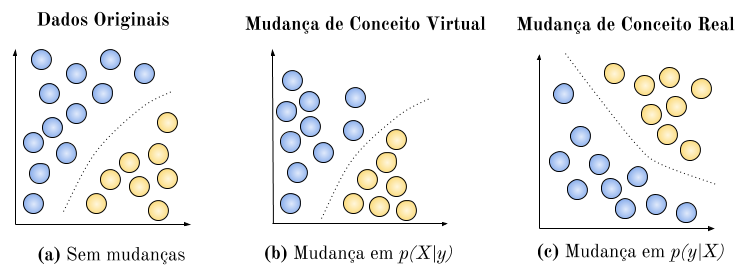
\includegraphics[scale=0.8]{imagens/concept_drift.png}
    \caption{Mudança de Conceito Virtual vs. Mudança de Conceito Real}
    \label{fig:real_and_virtual_concept_drift}
\end{center}
\end{figure}

Em \cite{Gama:2014:SCD:2597757.2523813}, o seguinte cenário é utilizado para explicar a diferença entre uma mudança de conceito real e uma virtual.
Considere um fluxo \textit{online} de anúncios do setor imobiliário.
Um usuário deseja classificar estes anúncios em relevantes e não relevantes.
Suponha que, à época, o usuário esteja buscando um novo apartamento. 
Isto torna anúncios de apartamentos residenciais mais relevantes e os anúncios de casa de férias menos relevantes.
Se o autor dos anúncios é alterado, o estilo de escrita sofre mudanças, mas os apartamentos permanecem relevantes para o usuário.
Este cenário corresponde a uma mudança de conceito virtual.
Considere que devido a uma crise, mais anúncios de apartamentos e menos de casas de férias aparecem, mas o editor dos anúncios permanece o mesmo.
Esta situação corresponde a uma mudança na probabilidade das classes.
Em outro cenário, assuma que o usuário acabou de comprar um apartamento e está em busca de um local para passar as férias.
Neste contexto, apartamentos tornaram-se irrelevantes e casas de férias, relevantes.
Apesar do editor dos anúncios e das probabilidades anteriores das classes permanecerem as mesmas, este cenário corresponde a uma mudança de conceito real.

Considerando apenas a perspectiva de predição, adaptações no modelo são necessárias apenas quando mudanças de conceito reais ocorrem, 
pois os limites de decisão do modelo corrente tornam-se obsoletos em relação aos novos eventos \cite{Gama:2014:SCD:2597757.2523813}.
Adaptação, neste contexto, significa atualizar o modelo de decisão perante a nova distribuição dos dados a fim de manter uma alta acurácia.

Mudanças de conceito podem se apresentar sob diferentes padrões.
Conforme ilustrado na Figura \ref{fig:concept_drift_patterns}, mudanças de conceito podem ocorrer de forma abrupta, gradual, incremental ou recorrente.
 
\begin{figure}[!ht]
\begin{center}
    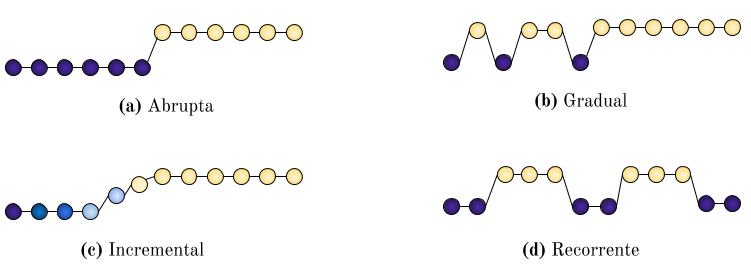
\includegraphics[scale=0.80]{imagens/concept_drift_patterns.png}
    \caption{Padrões de ocorrência de Mudanças de Conceito}
    \label{fig:concept_drift_patterns}
\end{center}
\end{figure}

Mudanças de conceito abruptas são alterações súbitas entre conceitos, como descrito na Figura \ref{fig:concept_drift_patterns} (a).
Por exemplo, o gênero literário de João pode subitamente mudar de ficção científica para auto-ajuda.
Outro exemplo, é a troca de um sensor por outro com diferente calibração, em uma planta industrial química \cite{Gama:2014:SCD:2597757.2523813}. 

Em constrate com a mudança de conceito abrupta, a mudança de conceito gradual significa uma transição mais lenta de um conceito para outro.
Isto é, durante a transição, são percebidos eventos de ambos os conceitos.
Pode-se considerar que João, ao invés de subitamente passar a preferir livros de auto-ajuda, adquire interesse nestes ao longo do tempo.
Isto significa que João ainda tem interesse em livros de ficção científica, mas desenvolve, em paralelo, um crescente interesse por livros de auto-ajuda, que se tornará predominante.
A mudança de conceito gradual está representada na Figura \ref{fig:concept_drift_patterns} (b).

Mudanças de conceito incrementais apresentam diversos conceitos intermediários durante a transição de um conceito para outro.
No exemplo de João, é como se o seu interesse literário variasse de ficção científica para ficção científica e aventura, 
de ficção científica e aventura para aventura e suspense, de aventura e suspense para suspense e auto-ajuda, e finalmente de suspense e auto-ajuda para apenas auto-ajuda.
Considerando a planta industrial química e os sensores, seria como se um sensor perdesse precisão ao longo do tempo. 
A Figura \ref{fig:concept_drift_patterns} (c) demonstra a mudança de conceito incremental. 

Existe ainda outro padrão, denominado mudança de conceito recorrente \cite{Zliobaite:2010}. 
Conforme apresentado na Figura \ref{fig:concept_drift_patterns} (d), a mudança de conceito recorrente existe quando um conceito previamente ativo, 
reaparece após determinado período de tempo.
De volta ao nosso exemplo, João está atualmente interessado em livros de ficção científica.
Contudo, ele é presenteado com uma série de livros de auto-ajuda de um renomado autor brasileiro.
Após ler toda a série, João é premiado com descontos para livros de ficção científica.
Ele, volta, então, a ler livros de ficção científica comprados com os descontos recebidos.

É importante destacar que o fenômeno Mudança de Conceito tem sido estudado em diferentes comunidades de pesquisa, incluindo mineração de dados, 
aprendizado de máquina, estatística e recuperação de informação \cite{Zliobaite:2010}.
Contudo, o mesmo conceito pode ter diferentes nomeclaturas em cada comunidade.
Na Tabela \ref{tbl:taxonomy} são listados os termos correspondentes a Mudança de Conceito para cada área de pesquisa.

\begin{center} 
\begin{table}[!ht]
\label{tbl:taxonomy}
\begin{tabularx}{\textwidth}{|l|X|}
\cline{1-2}
\multicolumn{1}{|c|}{\textbf{Área}} & \multicolumn{1}{c|}{\textbf{Termos}}       \\ \cline{1-2}
Mineração de Dados                  & Mudança de Conceito                        \\ \cline{1-2}
Aprendizado de Máquina              & Mudança de Conceito, Mudança de Covariável \\ \cline{1-2}
Computação Evolucionária            & Ambiente Evolutivo, Ambiente em Mudança    \\ \cline{1-2}
IA e Robótica                       & Ambiente Dinâmico                          \\ \cline{1-2}
Estatísticas, Séries Temporais      & Não Estacionário                           \\ \cline{1-2}
Recuperação de Informação           & Evolução Temporal                          \\ \cline{1-2}
\end{tabularx}
\caption{Terminologia - Mudança de Conceito \cite{Zliobaite:2010}}
\end{table}
\end{center}

Outra possível fonte de equívoco é a utilização dos termos Detecção de \textit{Outliers}, Detecção de Novidade e Detecção de \textit{Change Points}.
Estes termos apresentam relação para com Detecção de Mudança de Conceito, pois dizem respeito a encontrar padrões que são diferentes dos padrões conhecidos.
Em alguns contextos, esses termos são usados indistitamente, entretanto, neste trabalho eles serão diferenciados.

De acordo com \cite{Chandola:2009:ADS:1541880.1541882}, 
Detecção de \textit{Outliers} refere-se a tarefa de encontrar padrões nos dados que não estão de acordo com o comportamento esperado.
Esses padrões podem ser denominados como: \textit{outliers}, anomalias, observações discordantes, exceções, peculiaridades ou aberrações.

Para \cite{Gama:2010:KDD:1855075}, exemplos esparsos e independentes, cujas características diferem muito daqueles que definem o modelo, 
devem ser considerados como \textit{outliers}, pois não há garantia de que representem um conceito. 
Em \cite{Aggarwal:2003:FCE:1315451.1315460}, os autores tipificam os \textit{outliers} como anomalias ou ruídos.
As anomalias constituem um tipo especial de \textit{outlier}, que é de interesse dos analistas.
Contudo, conforme \cite{Gama:2010:KDD:1855075}, é necessário um grupo conciso de exemplos para evidenciar o aparecimento de um novo conceito, ou novidade.

Segundo \cite{Chandola:2009:ADS:1541880.1541882}, a Detecção de Novidade objetiva detectar padrões não observados (emergentes) nos dados.
Entretanto, esse termo se distingue da detecção de \textit{outliers}, pois os novos padrões, geralmente, são incorporados ao modelo.
Apesar de apresentarem definições próximas, a Detecção de Mudança de Conceito engloba a Detecção de Novidade e a extrapola, ao identificar 
mudanças de conceito reais a partir do \textit{feedback} sobre a performance preditiva \cite{Gama:2010:KDD:1855075}.

Técnicas para Detecção de \textit{Change Points} identificam variações abruptas de valor em séries temporais, que podem representar transições entre estados.
Diferenciam-se das técnicas para Detecção de Mudança de Conceito pois são aplicadas em séries temporais unidimensionais estacionárias \cite{Aminikhanghahi:2017:SMT:3086013.3086037}.

O método proposto neste projeto de mestrado objetiva identificar mudanças de conceito virtuais e reais, seja qual for o padrão de ocorrência.
Na seção seguinte serão detalhados os principais algoritmos para Detecção de Mudança de Conceito.

\subsection{Algoritmos para Detecção de Mudança de Conceito}

Os algoritmos para Detecção de Mudança de Conceito são os responsáveis por identificar, de forma explícita, as mudanças de conceito nos fluxos de dados \cite{Gama:2014:SCD:2597757.2523813}.
Estes métodos caracterizam e quantificam as mudanças de conceito através da delimitação dos instantes ou intervalos de tempo em que as mudanças ocorrem \cite{Basseville:1993:DAC:151741}.

As técnicas propostas na literatura podem ser divididas em duas categorias, baseado na dependência ou não de dados rotulados:
\begin{description}
    \item[Algoritmos Explícitos/Supervisionados] Dependem da rotulação dos dados por um especialista.
    Estes rótulos são utilizados no cálculo de medidas de performance como taxa de erro e acurácia, que são monitoradas ao longo do tempo.
    Mudanças de conceito são sinalizadas quando essas medidas atingem um limite previamente definido.

    \item[Algoritmos Implícitos/Não Supervisionados] Independem da rotulação por especialistas, 
    baseando-se em características dos próprios dados para sinalizar desvios.
    São mais propensos a alarmes falsos, mas a independência de rótulos os torna interessantes para contextos onde a obtenção desses é dispendiosa, demorada ou inviável.
\end{description}

Em sua pesquisa \cite{Gama:2014:SCD:2597757.2523813} categorizou os algoritmos supervisionados em três grupos principais:

\begin{description}
    \item[Métodos Baseados em Análise Sequencial] Avaliam, de forma sequenciada, os resultados das predições conforme tornam-se disponíveis (performance).
    Indicam a ocorrência de mudança de conceito quando um limite pré-definido é atingido.
    Os algoritmos \textit{Cumulative Sum (CUSUM)}, \textit{PageHinkley (PH)} \cite{Page:CUSUM:PageHinkley:1954} e \textit{Geometric Moving Average (GMA)} \cite{Roberts:2000:CCT:338441.338464}
    são representantes deste grupo.

    \item[Abordagens baseadas em Estatística] Identificam mudanças de conceito através da análise de parâmetros estatísticos como média e desvio padrão para os resultados das predições.
    Os métodos \textit{Drift Detection Method (DDM)} \cite{GamaMCR04}, 
    \textit{Early Drift Detection Method (EDDM)} \cite{EDDM}, 
    \textit{Exponentially Weighted Moving Average (EWMA)} \cite{Ross:2012:EWM:2076039.2076307} e 
    \textit{Reactive Drift Detection Method (RDDM)} \cite{Barros:RDDM:2017} são exemplos deste grupo.

    \item[Métodos baseados em Janelas] Geralmente, utilizam uma janela de tamanho fixo para sumarizar informações passadas e uma janela deslizante para sumarizar dados mais recentes.
    A mudança de conceito é detectada quando há uma diferença significativa entre as distribuições das janelas.
    Esta diferença é detectada a partir de testes estatísticos ou desigualdades matemáticas, considerando como hipótese nula a igualdade entre as distribuições.
    Os algoritmos 
    \textit{Adaptive Windowing (ADWIN)} \cite{BifetG07}, 
    \textit{SeqDrift} \cite{PearsSK14:SeqDrift:2014}, 
    \textit{HDDMA} e \textit{HDDMW} \cite{BlancoCRBDM15:HDDMA:HDDMW:2015}
    são membros desta família.
\end{description}

Os algoritmos implícitos também foram divididos em três grupos \cite{GONCALVES20148144}:

\begin{description}
    \item[Detecção de Novidade / Métodos de Agrupamento] 
    Utilizam a distância e/ou a densidade dos dados para detectar novos padrões.
    O algoritmo identifica exemplos suspeitos e os atribui a uma classe \textit{Desconhecido}, indicando a necessidade de uma avaliação adicional.
    As técnicas de agrupamento e detecção de \textit{outliers} são estratégias de implementação populares para estes algoritmos, 
    pois sintetizam os dados correntes e aplicam medidas de dissimilaridade para identificar novos padrões \cite{Ryu:Kantardzic:2012}.
    Os métodos 
    \textit{OLINDDA} \cite{Spinosa:2007:OCA:1244002.1244107},
    \textit{MINAS} \cite{Faria:2013:NDA:2480362.2480515},
    \textit{Woo} \cite{Ryu:Kantardzic:2012},
    \textit{DETECTNOD} \cite{Hashemi:Hayat:DETECTNOD:2010},
    \textit{ECSMiner} \cite{Masud:2011:CNC:1978259.1978529} e
    \textit{GC3} \cite{Sethi2016b:GC3} fazem parte deste grupo.
    
    \item[Monitoramento de distribuição multivariada]
    Monitoram diretamente a distribuição dos dados, considerando cada atributo.
    Este monitoramento é feito através de subconjuntos dos dados.
    Um subconjunto de treinamento tem sua distribuição sumarizada e armazenada, para ser utilizada como referência.
    A distribuição referência é comparada à distribuição do subconjunto atual e, havendo diferenças significativas, a mudança de conceito é sinalizada.
    Os algoritmos
    \textit{CoC} \cite{Lee:Magoules:CoC:2012},
    \textit{HDDDM} \cite{Ditzler:Polikar:HDDDM:2011},
    \textit{PCA-detect} \cite{Kuncheva:PCADetect:20085}
    são representantes deste grupo.

    \item[Monitoramento dependente de modelo]
    As técnicas elencadas nos grupos anteriores monitoram desvios na distribuição dos dados para indicar mudanças de conceito.
    Essencialmente, esses métodos assumem que alterações na distribuição $P(X)$ implicarão mudanças na performance do classificador $p(y|X)$.
    Apesar de permitir a aplicação de qualquer tipo de classificador, essa presunção leva a uma maior quantidade de falsos positivos.
    As técnicas dependentes de modelo, por sua vez, restringem-se aos classificadores probabilísticos,
    o que permite realizar a detecção de mudanças de conceito através do monitoramento das probabilidades a posteriori \cite{Zliobaite:2010}.
    A utilização das probabilidades a posteriori diminui a incidência de falsos positivos e torna o processo computacionalmente eficiente, 
    pois apenas um único fluxo univariado de valores é observado.
    Os métodos 
    \textit{A-distance} \cite{Dredze:ADistance:2010585},
    \textit{CDBD} \cite{Lindstrom:CDBD:2013} e
    \textit{Margin} \cite{Dries:Margin:2009} participam deste grupo.
\end{description}

Por fim, a Tabela \ref{tbl:abordagens} sumariza as categorias, os grupos e as respectivas técnicas mencionadas nesta seção.

% Please add the following required packages to your document preamble:
% \usepackage{graphicx}
\begin{table}[!ht]
    \centering
    \resizebox{\textwidth}{!}{%
    \begin{tabular}[t]{@{}lllll@{}}
    \hline \\
    Algoritmos Explícitos/Supervisionados     & Métodos Baseados em Análise Sequencial        & \begin{tabular}[t]{@{}l@{}} Cumulative Sum (CUSUM) \\ PageHinkley (PH) \cite{Page:CUSUM:PageHinkley:1954} \\ Geometric Moving Average (GMA) \cite{Roberts:2000:CCT:338441.338464}\end{tabular}                                                                                                                        &  &  \\ \\
                                              & Abordagens baseadas em Estatística            & \begin{tabular}[t]{@{}l@{}} Drift Detection Method (DDM) \cite{GamaMCR04} \\  Early Drift Detection Method (EDDM) \cite{EDDM} \\  Exponentially Weighted Moving Average (EWMA) \cite{Ross:2012:EWM:2076039.2076307} \\ Reactive Drift Detection Method (RDDM) \cite{Barros:RDDM:2017} \end{tabular}                                                                &  &  \\ \\
                                              & Métodos baseados em Janelas                   & \begin{tabular}[t]{@{}l@{}} Adaptive Windowing (ADWIN) \cite{BifetG07} \\   SeqDrift \cite{PearsSK14:SeqDrift:2014} \\   HDDMA/HDDMW \cite{BlancoCRBDM15:HDDMA:HDDMW:2015} \end{tabular}                                                                                            &  &  \\ \\
    
    Algoritmos Implícitos/Não Supervisionados & Detecção de Novidade / Métodos de Agrupamento & \begin{tabular}[t]{@{}l@{}} OLINDDA \cite{Spinosa:2007:OCA:1244002.1244107} \\   MINAS \cite{Faria:2013:NDA:2480362.2480515} \\   Woo \cite{Ryu:Kantardzic:2012} \\   DETECTNOD \cite{Hashemi:Hayat:DETECTNOD:2010} \\   ECSMiner \cite{Masud:2011:CNC:1978259.1978529} \\   GC3 \cite{Sethi2016b:GC3} \end{tabular} &  &  \\ \\
                                              & Monitoramento de distribuição multivariada    & \begin{tabular}[t]{@{}l@{}} CoC \cite{Lee:Magoules:CoC:2012} \\ HDDDM \cite{Ditzler:Polikar:HDDDM:2011} \\ PCA-detect \cite{Kuncheva:PCADetect:20085} \end{tabular}                                       &  &  \\ \\
                                              & Monitoramento dependente de modelo            & \begin{tabular}[t]{@{}l@{}} A-distance \cite{Dredze:ADistance:2010585} \\ CDBD \cite{Lindstrom:CDBD:2013} \\ Margin \cite{Dries:Margin:2009} \end{tabular}                                                                                        &  &  \\ \\
    \hline
    \end{tabular}%
    }
    \caption{Sumário - Abordagens de detecção \cite{Sethi:2017:RDC:3096751.3096864}}
    \label{tbl:abordagens}
\end{table}

O algoritmo desenvolvido neste projeto de mestrado enquadra-se na categoria de algoritmos implícitos ou não supervisionados, mais especificamente no grupo \textit{Detecção de Novidades / Métodos de Agrupamento}.
Na próxima seção, abordaremos as ferramentas utilizadas para implementação da técnica e sua validação.

\subsection{Ferramentas}

Nesta seção, os frameworks \textit{Massive Online Analysis} (MOA) e \textit{Tornado} serão apresentados.
Estes frameworks possibilitam a implementação e a análise - perante o estado da arte - de algoritmos para detecção de mudança de conceito.
Ambos permitem a avaliação entre técnicas e a utilização de diferentes \textit{datasets}.

\subsection{MOA}

O \textit{MOA – Massive Online Analysis}\footnote{https://moa.cms.waikato.ac.nz/} é, atualmente, o principal framework para mineração de dados em fluxos contínuos.
O projeto é de código-aberto\footnote{https://github.com/Waikato/moa} e apresenta uma comunidade bastante ativa e crescente \cite{Bifet:2010:MMO:1756006.1859903}.
A aplicação é composta por uma ampla coleção de algoritmos da área de aprendizado de máquina: classificação, regressão, agrupamento, busca por padrões, detecção de \textit{outliers}, detecção de mudanças de conceito e sistemas de recomendação.
Além de conter ferramentas para avaliação destes.
Apresenta relação com o projeto WEKA \cite{Hall:2009:WDM:1656274.1656278}, sendo também desenvolvido em Java, o que permite a sua execução nos principais sistemas operacionais.

O MOA divide suas funcionalidades em tarefas (\textit{tasks}).
As principais tarefas incluem:
produção de fluxos de dados,
treino de classificadores,
aplicação de algoritmos de agrupamento,
análise de algoritmos para detecção de \textit{outliers} e de \textit{concept drift}, dentre outras.
As tarefas podem ser executadas a partir da interface gráfica (GUI) ou por linha de comando.
A tela principal da aplicação é demonstrada na Figura \ref{fig:moa}.
Através da interface gráfica é possível executar múltiplas tarefas de forma concorrente, 
controlar suas execuções e visualizar os resultados parciais.

\begin{figure}[!ht]
\begin{center}
    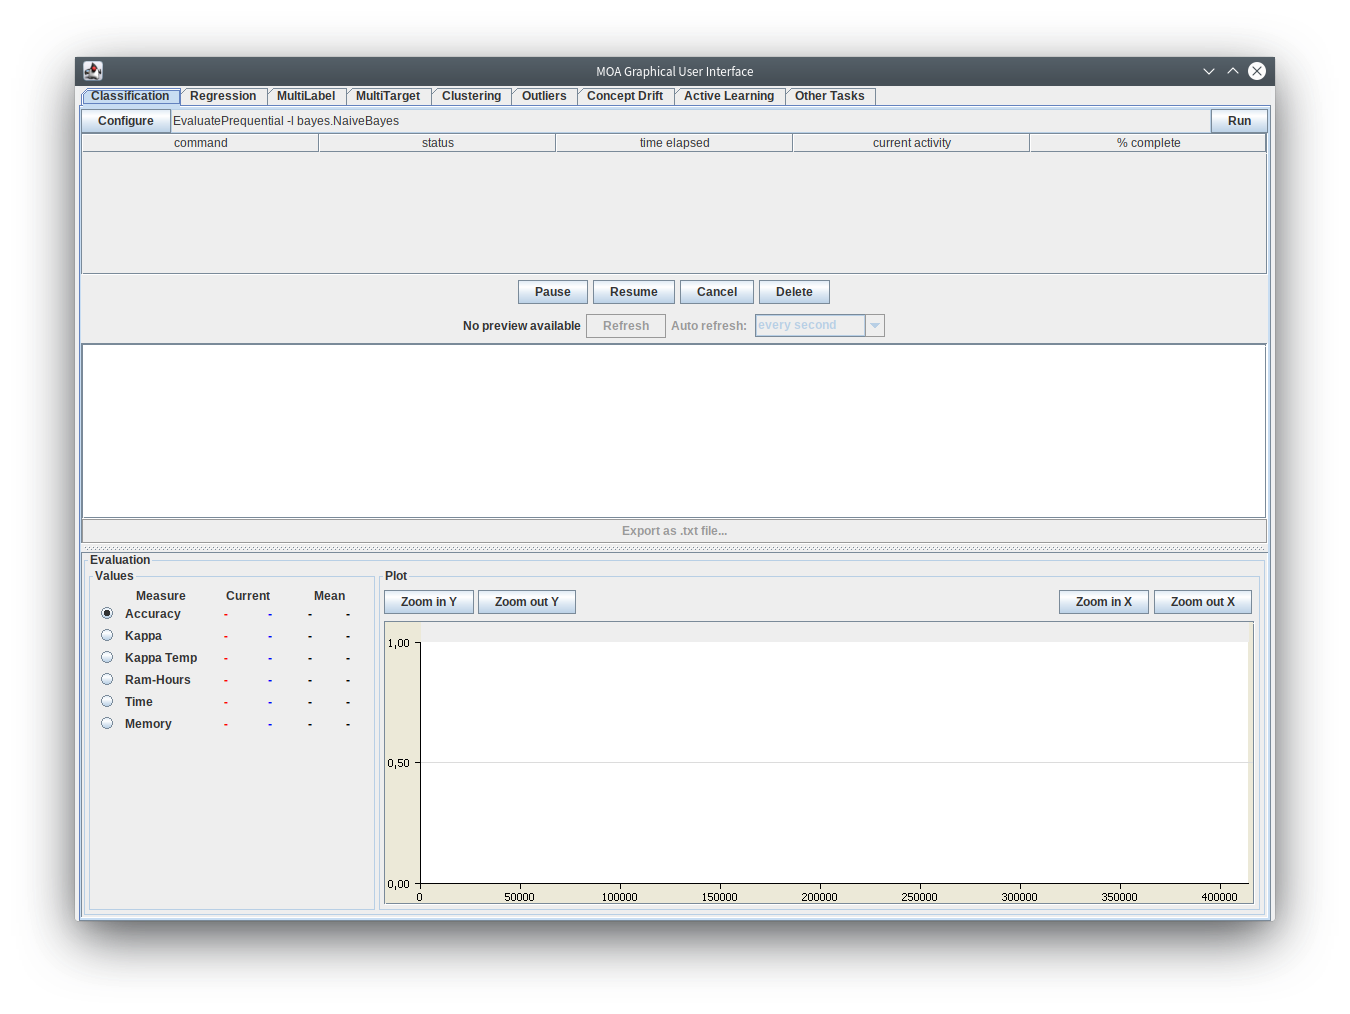
\includegraphics[scale=0.5]{imagens/moa.png}
    \caption{MOA - Tela Inicial}
    \label{fig:moa}
\end{center}
\end{figure}

A aplicação é capaz de ler arquivos em formato \textit{ARFF}, populares por serem utilizados no projeto WEKA \cite{Hall:2009:WDM:1656274.1656278}.
A ferramenta também permite a produção de fluxos de dados dinamicamente, através de geradores.
Alguns dos geradores de fluxo disponíveis no MOA são:
\textit{Random Trees} \cite{Domingos:2000:MHD:347090.347107}
\textit{SEA} \cite{Street:2001:SEA:502512.502568}, 
\textit{STAGGER} \cite{Schlimmer1986}, 
\textit{Rotating Hyperplane} \cite{Wang:2003:MCD:956750.956778},
\textit{Random RBF}, 
\textit{LED} \cite{Gama:2003:ADT:956750.956813}, 
\textit{Waveform} \cite{Gama:2003:ADT:956750.956813}, 
 e \textit{Function} \cite{Jin:2003:EDT:956750.956821}.

Outra característica interessante do framework é a possibilidade de adicionar mudanças de conceito a fluxos estacionários existentes.
Isto é feito através de uma função sigmóide, que modela o evento de mudança de conceito como uma combinação balanceada de duas distribuições homogêneas, 
que caracterizam os conceitos alvo antes e depois da mudança \cite{bifet2009data}.
Além destes conceitos, o usuário também pode definir o momento da mudança e a sua duração \cite{Bifet:2010:MMO:1756006.1859903}.

Os principais métodos para detecção de mudança de conceito propostos na literatura estão disponíveis no MOA.
O framework também permite a utilização de classificadores do WEKA \cite{Hall:2009:WDM:1656274.1656278} combinados aos detectores.
A janela para configuração de um detector é demonstrada na Figura \ref{fig:moa_detector}.

\begin{figure}[!ht]
\begin{center}
    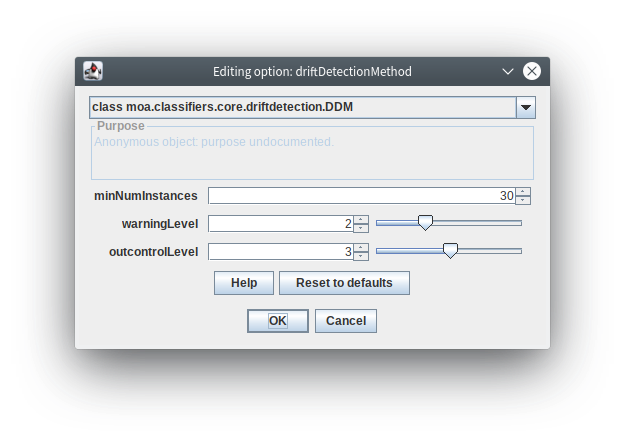
\includegraphics[scale=1]{imagens/detector.png}
    \caption{MOA - Configuração detector}
    \label{fig:moa_detector}
\end{center}
\end{figure}

A arquitetura do framework é modular, o que permite aos usuários implementar novas tarefas com pouco esforço.
Por exemplo, para criar um novo detector, basta estender a classe abstrata \texttt{moa.classifiers.core.driftdetection.AbstractChangeDetector} e implementar o algoritmo desejado.
A janela de configuração para o detector (similar a \ref{fig:moa_detector}) é criada dinamicamente, a partir dos atributos da classe.

O MOA dispõe de diversas classes para avaliação de técnicas de aprendizado de máquina. 
Para este trabalho, destacam-se as classes \texttt{DriftDetectionMethodClassifier} e \texttt{BasicConceptDriftPerformanceEvaluator}, 
que realizam a análise de algoritmos para detecção de mudança de conceito.
A classe \texttt{DriftDetectionMethodClassifier} permite avaliar técnicas de detecção que encapsulam um classificador.
Por sua vez, a classe \texttt{BasicConceptDriftPerformanceEvaluator} avalia a performance das técnicas de detecção diretamente, 
sem a necessidade de um classificador.
Estes avaliadores e os seus indicadores serão detalhados juntamente com os resultados dos experimentos iniciais, na Seção \ref{experimentos_iniciais}. 

Neste projeto de mestrado foram implementados novos detectores para o MOA e as duas técnicas de validação foram utilizadas na análise dos experimentos.

\subsection{Tornado}

O Tornado é, assim como o MOA, um framework para mineração de dados para fluxos contínuos \cite{Pesaranghader:Tornado}.
O projeto é desenvolvido na linguagem Python e seu código está disponível\footnote{https://github.com/alipsgh/tornado}.
O framework diferencia-se do MOA por apresentar um cenário de avaliação específico: 
analisar a execução, em paralelo, de pares (classificador, detector de mudança de conceito), 
para identificar o par ótimo ao longo do tempo, em relação ao fluxo de dados.

\begin{figure}[!ht]
\begin{center}
    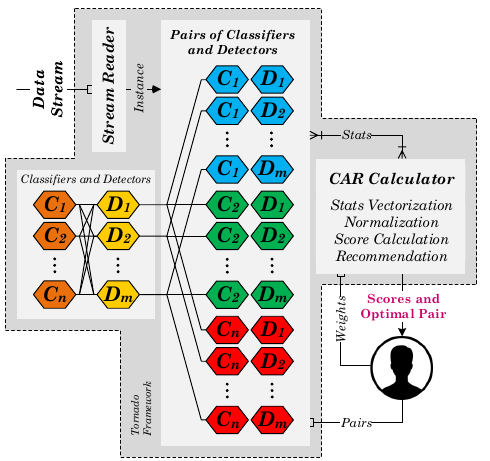
\includegraphics[scale=0.75]{imagens/tornado.png}
    \caption{Framework Tornado \cite{Pesaranghader:Tornado}.}
    \label{fig:tornado}
\end{center}
\end{figure}

Conforme apresentado na Figura \ref{fig:tornado}, os principais componentes do framework são: 
\textit{Stream Reader}, \textit{Classifiers}, \textit{Detectors}, \textit{Classifier-Detector Pairs} e \textit{CAR Calculator}.
A entrada de dados é composta por um fluxo (\textit{Stream}), uma lista de pares (classificador, detector) e um vetor com pesos.
O Tornado utiliza a abordagem de validação \textit{prequential}, na qual as instâncias são testadas e depois utilizadas no aprendizado \cite{Gama:2014:SCD:2597757.2523813}.

O componente \textit{Stream Reader} lê instâncias a partir do fluxo e as envia, uma a uma, para o par (classificador, detector), para construção do modelo.
Os modelos são construídos de forma incremental. Por seguir a abordagem \textit{prequential}, cada instância é primeiramente utilizada para testes e depois como treinamento.
Simultaneamente, os classificadores enviam suas estatísticas (taxas de erro ou resultados das predições) aos detectores, para que a mudança de conceito possa ser sinalizada.
Por fim, o componente \textit{CAR Calculator} calcula uma pontuação para cada par, considerando taxas de erro, atraso para detecção da mudança de conceito, falsos positivos, falsos negativos, quantidade de memória utilizada e tempo de execução \cite{Pesaranghader:Tornado}.
O framework apresenta ao usuário o par com maior pontuação. Este par, contudo, pode mudar devido ao aprendizado incremental ou à mudança de conceito.
A Figura \ref{fig:tornado_out2} apresenta um exemplo de resultado obtido através do framework.

\begin{figure}[!ht]
\begin{center}
    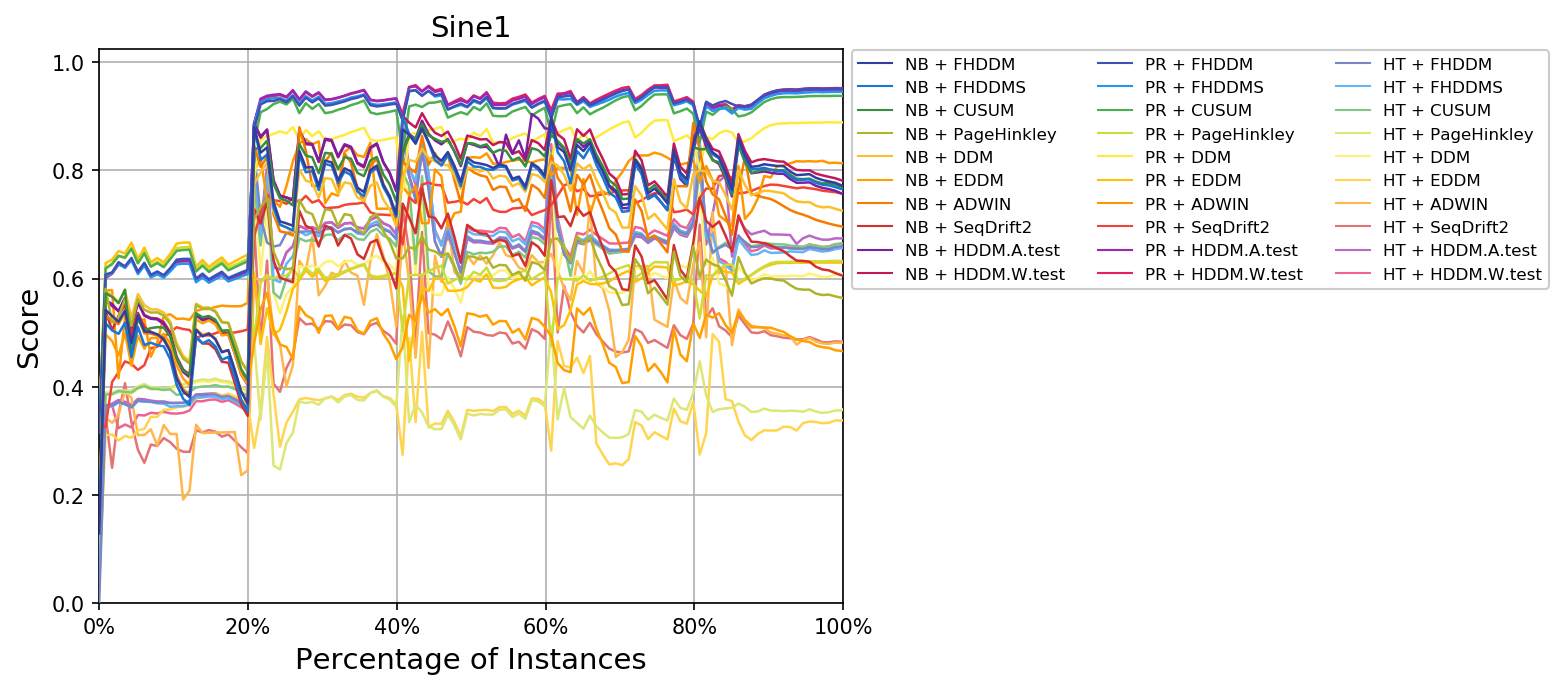
\includegraphics[scale=0.5]{imagens/tornado_out2.png}
    \caption{Tornado - Resultado para múltiplos pares \cite{Pesaranghader:Tornado}}
    \label{fig:tornado_out2}
\end{center}
\end{figure}

Neste trabalho de pesquisa, de forma similar ao MOA, a técnica proposta foi implementada no framework Tornado.
O framework foi utilizado na validação dos experimentos, permitindo verificar o comportamento do detector em conjunto com um classificador, ao longo do tempo.
Na seção seguinte, detalharemos conceitos sobre as Redes de Função de Base Radial, técnica que serviu de base para o algoritmo proposto nesta pesquisa.

\section{Redes de Função de Base Radial}

As Redes de Função de Base Radial (RBF \textit{networks}) são aproximadoras universais de funções.
As RBFs têm como principal diferença em relação às outras redes neurais, a forma de ativação.
Nessas redes, este processo é feito através do cálculo da distância entre os vetores de entrada e os centros estabelecidos \cite{Braga:RedesNeuraisTeoriaAplicacoes}.

Em sua forma básica, a arquitetura de uma rede do tipo RBF é composta por três camadas: 
uma camada de entrada, uma intermediária e uma de saída \cite{Rojas:1996:NNS:235222}. 
A camada intermediária (oculta) de uma RBF utiliza funções de base radiais para agrupar os dados de entrada em clusters, 
transformando padrões de entrada não linearmente separáveis em um conjunto de saídas linearmente separáveis. 
A camada de saída classifica os padrões recebidos através da combinação linear das saídas das funções \cite{Braga:RedesNeuraisTeoriaAplicacoes}.
A Figura \ref{fig:rbg_arq} demonstra essa arquitetura.

\begin{figure}[!ht]
\begin{center}
    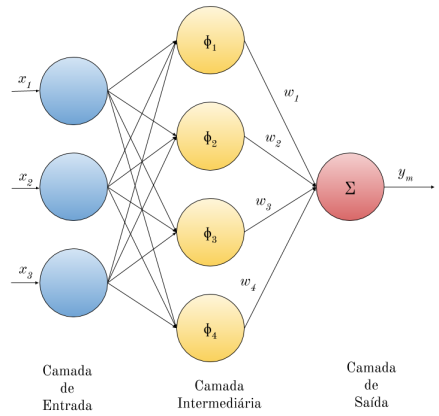
\includegraphics[scale=1]{imagens/rbf_arq.png}
    \caption{Arquitetura RBF}
    \label{fig:rbg_arq}
\end{center}
\end{figure}

Na literatura, a função de base radial Gaussiana (Eq. \ref{eq:gaussiana}) é uma das mais utilizadas para camada intermediária.

\begin{equation} \label{eq:gaussiana}
    f(x)=e^{-{\frac {v^{2}}{2\sigma^{2}}}}
\end{equation}

Na equação \ref{eq:gaussiana}, $v = \lVert x - t_i \rVert$ é dado pela distância euclidiana, onde $x$ é o valor de entrada da rede, 
enquanto $t_i$ e $\sigma$ correspondem respectivamente ao centro e a largura da função radial. 
Dessa maneira, a resolução de um determinado problema por uma rede do tipo RBF consiste na resolução das funções \ref{eq:rbf1} e
\ref{eq:rbf2} obtendo o sistema \ref{eq:rbf3}.

\begin{equation} \label{eq:rbf1}
    f(x)=\sum _{{i=1}}^{N}w_{ij}\varphi (||{\mathbf  {x}}-{\mathbf  {t}}_{i}||)
\end{equation}

\begin{equation} \label{eq:rbf2}
    y_i=\sum _{{i=1}}^{N}w_{ij}\phi (||{\mathbf  {x}}-{\mathbf  {t}}_{i}||) + w_{j_0}
\end{equation}

\begin{equation} \label{eq:rbf3}
\begin{bmatrix}
    \varphi (||{{x_1}}-{{t}}_{1}||) & \varphi (||{{x_1}}-{{t}}_{2}||) & \dots & \varphi (||{{x_1}}-{{t}}_{N}||) \\
    \varphi (||{{x_2}}-{{t}}_{1}||) & \varphi (||{{x_2}}-{{t}}_{2}||) & \dots & \varphi (||{{x_2}}-{{t}}_{N}||) \\
    \hdotsfor{5} \\
    \varphi (||{{x_N}}-{{t}}_{1}||) & \varphi (||{{x_N}}-{{t}}_{2}||) & \dots & \varphi (||{{x_N}}-{{t}}_{N}||)
\end{bmatrix}
\begin{bmatrix}
    w_1 \\
    w_2 \\
    \vdots \\
    w_N \\
\end{bmatrix}
=
\begin{bmatrix}
    y_1 \\
    y_2 \\
    \vdots \\
    y_N \\
\end{bmatrix}
\end{equation}

onde $w_{ij}$ são os pesos de cada conexão, $\phi$ é a matriz de interpolação originada do conjunto de $N$ funções
de base radial aplicadas nas entradas $x$ e dos seus respectivos centros $t_i$,
$w_{j_0}$ representa o bias, $\varphi (||{{x}}-{{t}}_{i}||)$ é o conjunto de $N$ funções de base radial,
$||\ldots||$ é a norma euclidiana e $y$ são as saídas geradas pela rede.

As camadas inicial e intermediária e suas propriedades de agrupamento são utilizadas como base para o algoritmo de detecção de mudança de conceito 
proposto neste projeto de mestrado. 

\section{Trabalhos Relacionados}

Além das referências básicas apresentadas nesta seção, foi realizada uma pesquisa na literatura visando identificar trabalhos relacionados 
que propõem a identificação de mudanças de conceito em FCDs através da aplicação de redes RBF, ou técnicas similares.

Em \cite{Jianping:Venkateswarlu:RBF:SpeakerIdentification} redes RBF com funções Gaussianas são utilizadas para detecção de novidades.
Os centros e as matrizes de covariância são definidas através do agrupamento via \textit{k-means} juntamente com a aplicação de heurísticas de largura ou do algoritmo \textit{EM}.
O método proposto não atua sobre fluxos de dados e constitue uma rede RBF completa e estática ao longo do tempo.

Roberts e Penny \cite{Roberts:Penny:Novelty:Confidence} propõem  um método para detecção de novidade baseado no monitoramento das taxas de erro e confiança, 
utilizando um comitê de redes RBF. 
Cada rede é inicializada com um vetor de pesos diferente.
A taxa de erro final é calculada a partir da matriz de covariância de erro do cômite criado.
Esta abordagem foi testada na classificação de pacientes com problemas de tremor muscular.

As RBFs também foram aplicadas para detecção de anomalias \cite{Bazargani2018RadialBF}.
Esta pesquisa realiza modificações às funções de perda (\textit{loss}) das redes, 
fazendo com que a rede atuem como classificador de classe única, 
permitindo a identificação de exemplos divergentes do padrão conhecido.

Este projeto de mestrado se diferencia dos trabalhos mencionados por utilizar apenas as camadas de entrada e intermediária das redes RBF para detecção de mudanças de conceito.
Além disso, etapas como a escolha dos centros e o cálculo do tamanho do raio são realizadas de forma dinâmica.
Estas características viabilizam a aplicação da técnica em fluxos contínuos de dados.

\section{Considerações Finais}

Neste capítulo foram apresentados alguns conceitos básicos que serão utilizados como base para a execução deste trabalho. 
Foram descritos os conceitos de 
Fluxos Contínuos de Dados e suas aplicações em Aprendizado de Máquina,
Mudança de Conceito,
técnicas para Detecção de Mudança de Conceito,
principais ferramentas da área e 
Redes de Função de Base Radial.
Por fim,
foram discutidos trabalhos que aplicam redes RBF para detecção de padrões divergentes (novidades, \textit{outliers}, etc).

\xchapter{Plano de Pesquisa}{} \label{plano_pesquisa}
\section{Considerações Iniciais}

Este capítulo descreve como a pesquisa proposta neste mestrado será desenvolvida para permitir que Redes de Função de Base Radial sejam aplicadas para detecção de mudanças de conceito em Fluxos Contínuos de Dados.
Espera-se que com a utilização das camadas inicial e intermediária das redes RBF e suas propriedades de agrupamento, seja possível detectar mudanças de conceito de forma eficiente e sem requerer a manutenção de estados prévios.
A seguir, são apresentados detalhes sobre cada etapa do desenvolvimento do projeto.

\section{Descrição do Problema}

O fenômeno Mudança de Conceito pode ser definido a partir do teorema de Bayes para probabilidades posteriores.
Seja $X$ um vetor de entrada e $Y$ a classe alvo,
a decisão de classificar $X$ como $Y$ dependerá da probabilidade posterior da classe, dada por:

\begin{equation} \label{eq:gaussiana}
    P(Y |X) = \frac{P(Y)P(X|Y)}{P(X)}
\end{equation}

onde $P(Y|X)$ é a probabilidade de $Y$ para a entrada $X$, $P(X|Y)$ é a distribuição condicional da classe para as variáveis da entrada $X$ e 
$P(Y)$ é a probabilidade a priori da classe e $P(X)$ é a probibilidade a priori do vetor de entrada $X$.

Na presença de mudança de conceito, a probabilidade posterior $P(Y|X)$ varia ao longo do tempo, isto é $P_{t_0}(Y|X)$ pode ser diferente de $P_{t_1}(Y|X)$.
Em outras palavras, os limites de decisão do classificador se alteram ao longo do tempo.

Considerando que redes de função de base radial apresentam em suas camadas inicial e intermediária características de agrupamento, 
este projeto de mestrado visa comprovara hipótese que redes RBF podem detectar mudanças de conceito em fluxos contínuos de dados, 
em tempo de execução, sem requerer a manutenção de estados prévios, de forma ágil e com precisão satisfatória.

Para exemplificar a execução desta proposta de mestrado, considere \ldots


\section{Atividades de Pesquisa}
\blindtext

\section{Considerações Finais}
\blindtext

\xchapter{Experimentos Iniciais}{} \label{experimentos_iniciais}
\section{Considerações Iniciais}
\blindtext

\section{Configuração dos Experimentos}
\blindtext

\section{Método de Pettitt}
\blindtext

\section{Redes de Função de Base Radial}
\blindtext

\section{Considerações Finais}
\blindtext


%% Parte pos-textual
\backmatter

% Bibliografia
% É aconselhável utilizar o BibTeX a partir de um arquivo, digamos "biblio.bib".
% Para ajuda na criação do arquivo .bib e utilização do BibTeX, recorra ao
% BibTeXpress em www.cin.ufpe.br/~paguso/bibtexpress
\bibliographystyle{abntex2-alf}
\bibliography{biblio}

% Apendices
% Comente se naoo houver apendices
%\appendix

%\xchapter{Exemplo de Ap\^endice}{} %sem preambulo
%\lipsum
% Eh aconselhavel criar cada apendice em um arquivo separado, digamos
% "apendice1.tex", "apendice.tex", ... "apendiceM.tex" e depois
% inclui--los com:
%\xchapter{Decomposição das séries temporais}{} %sem preambulo
\label{apendice1}
\section{Considerações Iniciais}
Neste apêndice consta as 40 séries temporais utilizadas nos experimentos mostrados no Capitulo \ref{experimentos}. As séries foram divididas em 4 tipos conforme a Tabela \ref{series}, onde o tipo representa um conjunto de 10 séries senoide ou cossenoide, sendo acrescida de ruído ou acrescida de ruído e tendência.
Nas imagens são representadas, a séries original,   seu componente determinístico e seu componente estocástico, os quais foram extraídos após a decomposição.
\section{Séries TIPO 1}
10 séries cossenoide com ruído ao longo da série.
\graphicspath{{imagens/}}
\begin{figure}[H]
\begin{center}
  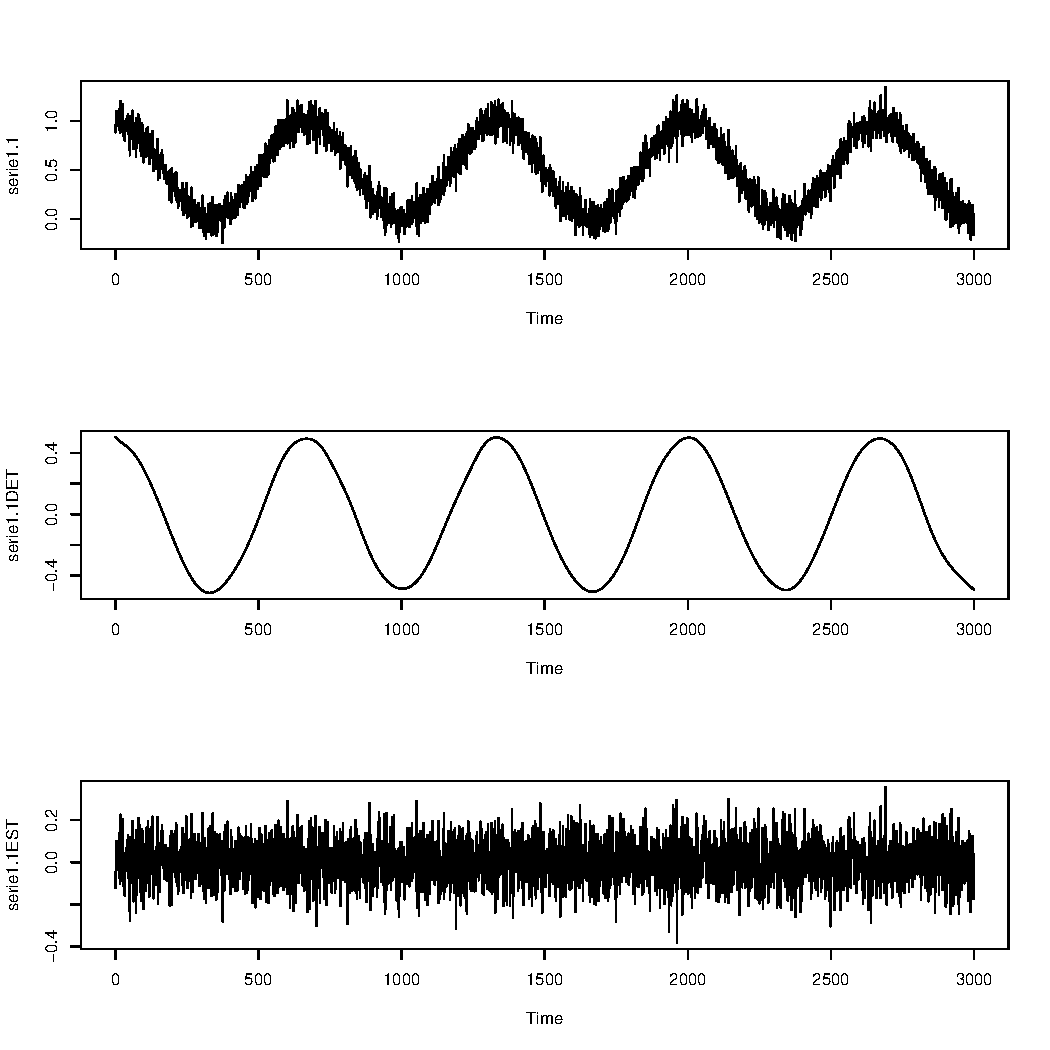
\includegraphics[scale=0.43]{serie1_1.pdf} \quad
  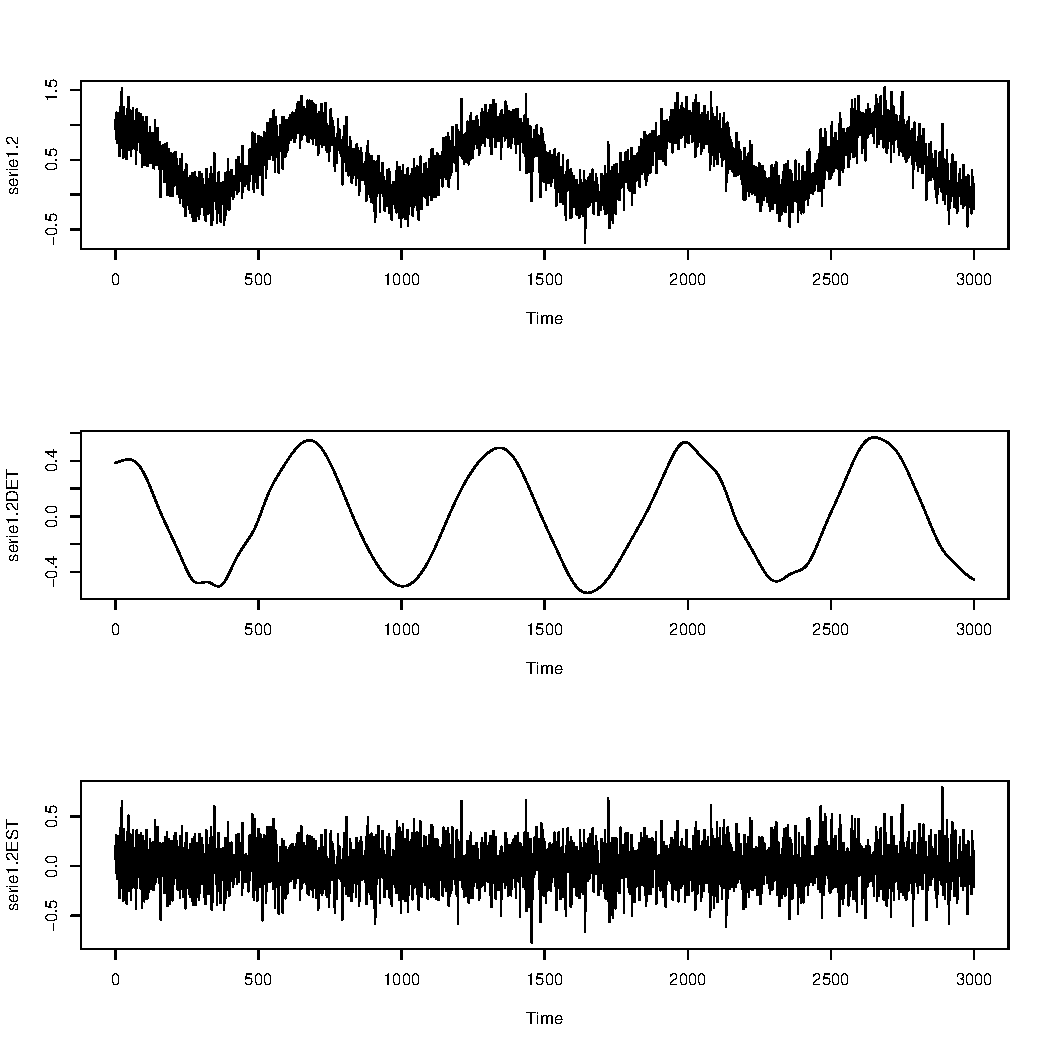
\includegraphics[scale=0.43]{serie1_2.pdf}
  \caption{Série 1.1 e Série 1.2}

\end{center}
\end{figure}

\graphicspath{{imagens/}}
\begin{figure}[H]
\begin{center}
  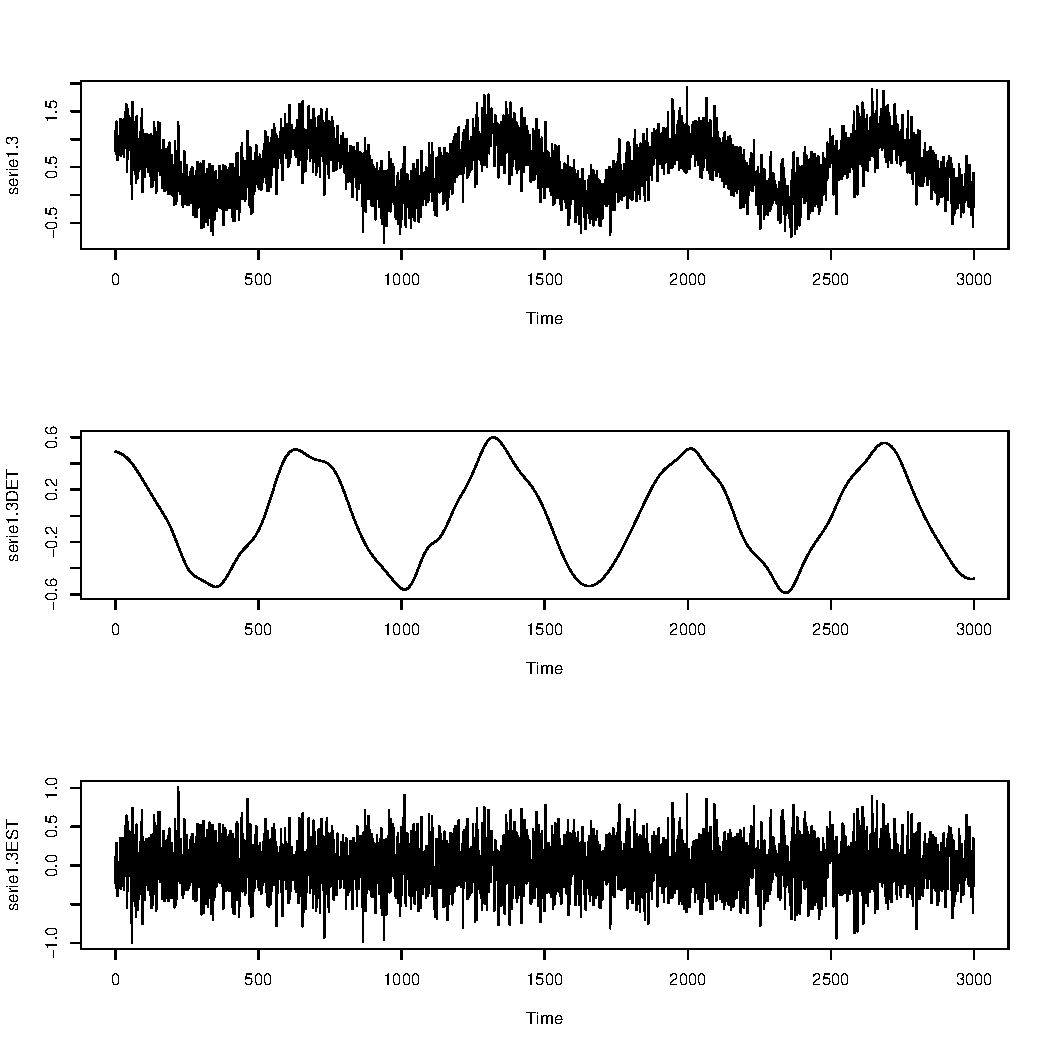
\includegraphics[scale=0.43]{serie1_3.pdf} \quad
  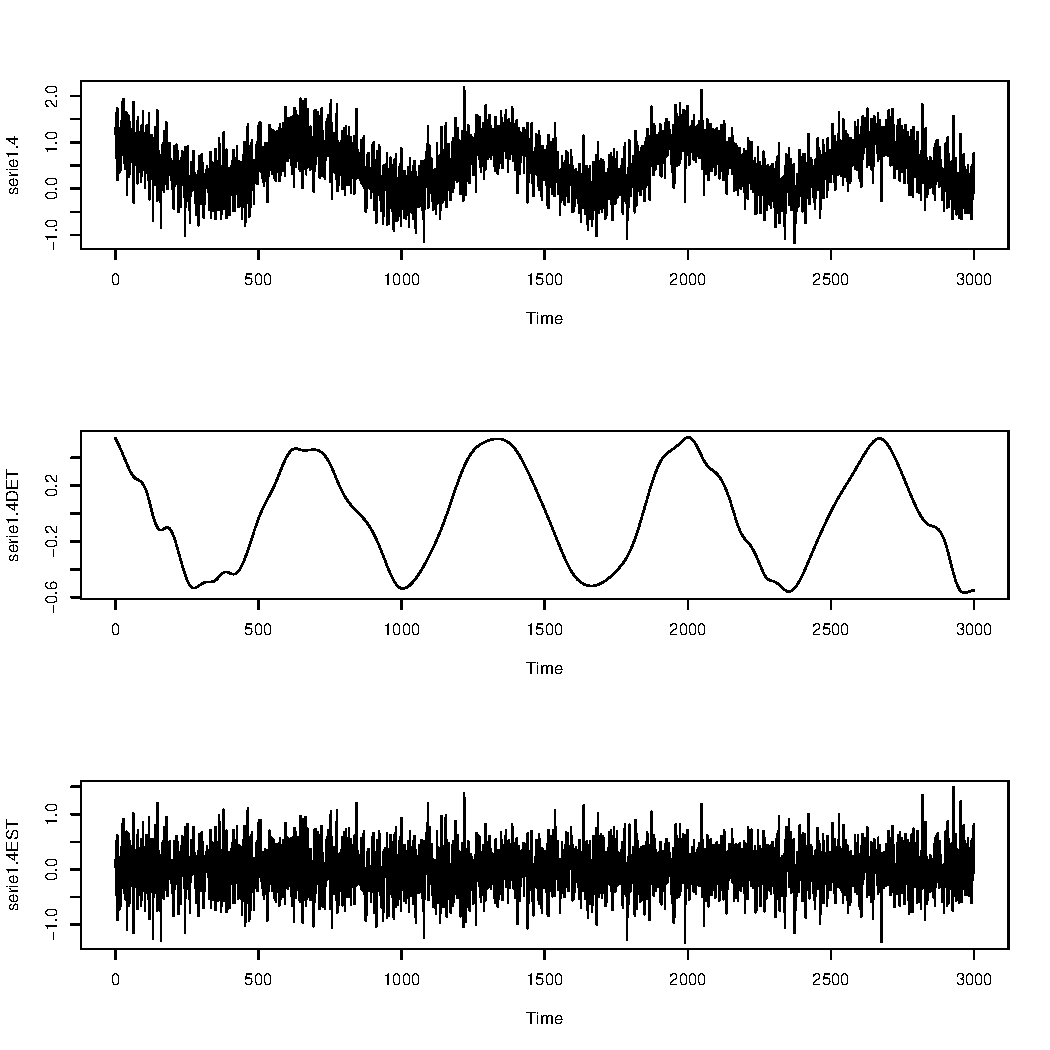
\includegraphics[scale=0.43]{serie1_4.pdf}
  \caption{Série 1.3 e Série 1.4}

\end{center}
\end{figure}

\graphicspath{{imagens/}}
\begin{figure}[H]
\begin{center}
  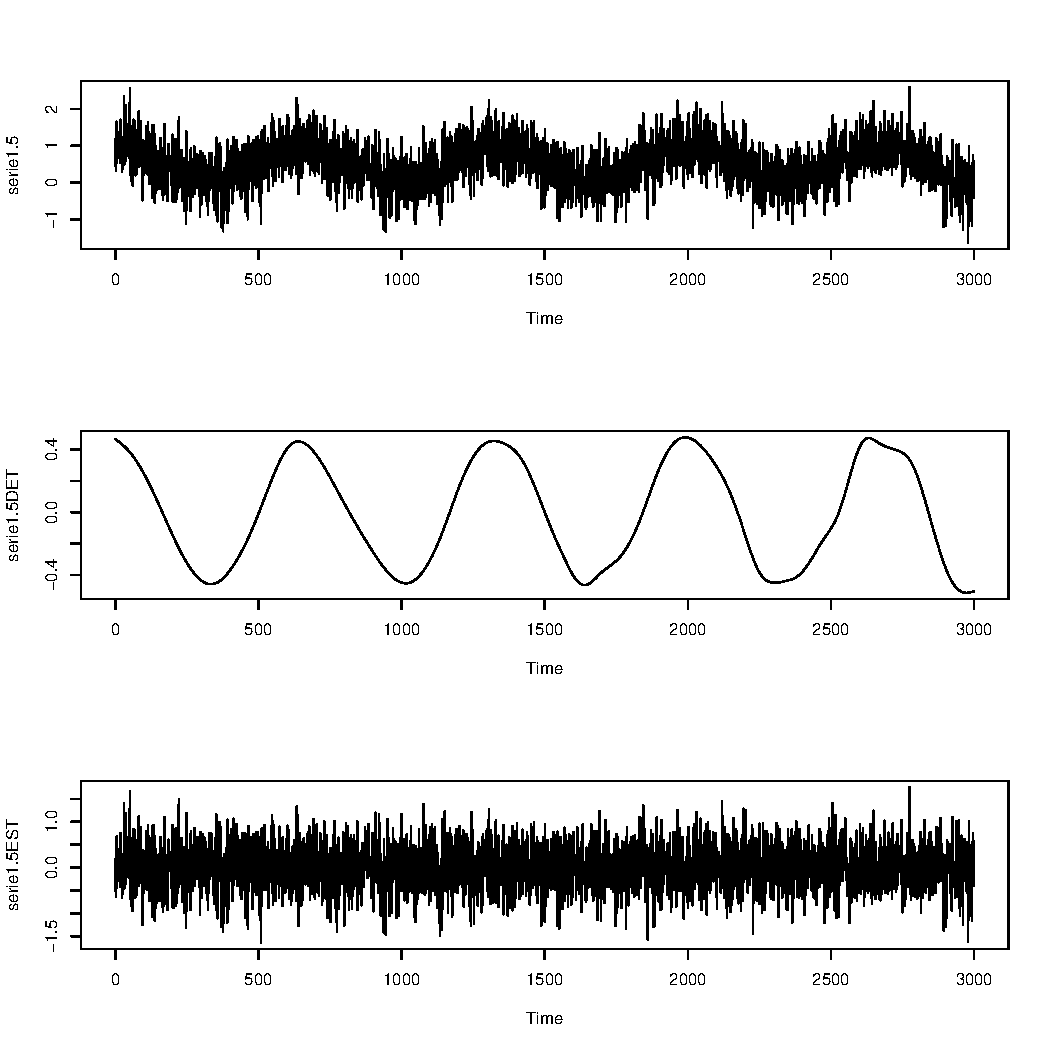
\includegraphics[scale=0.43]{serie1_5.pdf} \quad
  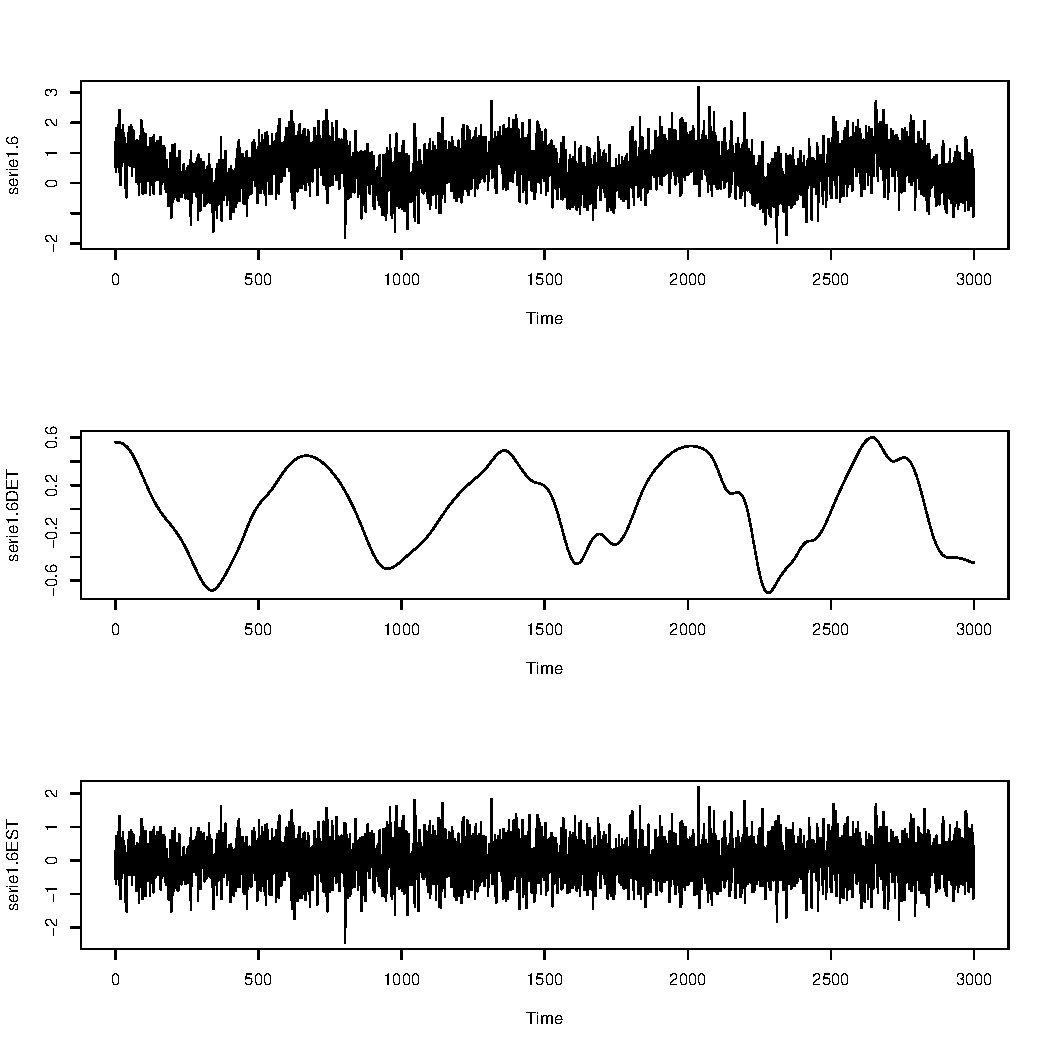
\includegraphics[scale=0.43]{serie1_6.pdf}
  \caption{Série 1.5 e Série 1.6}

\end{center}
\end{figure}

\graphicspath{{imagens/}}
\begin{figure}[H]
\begin{center}
  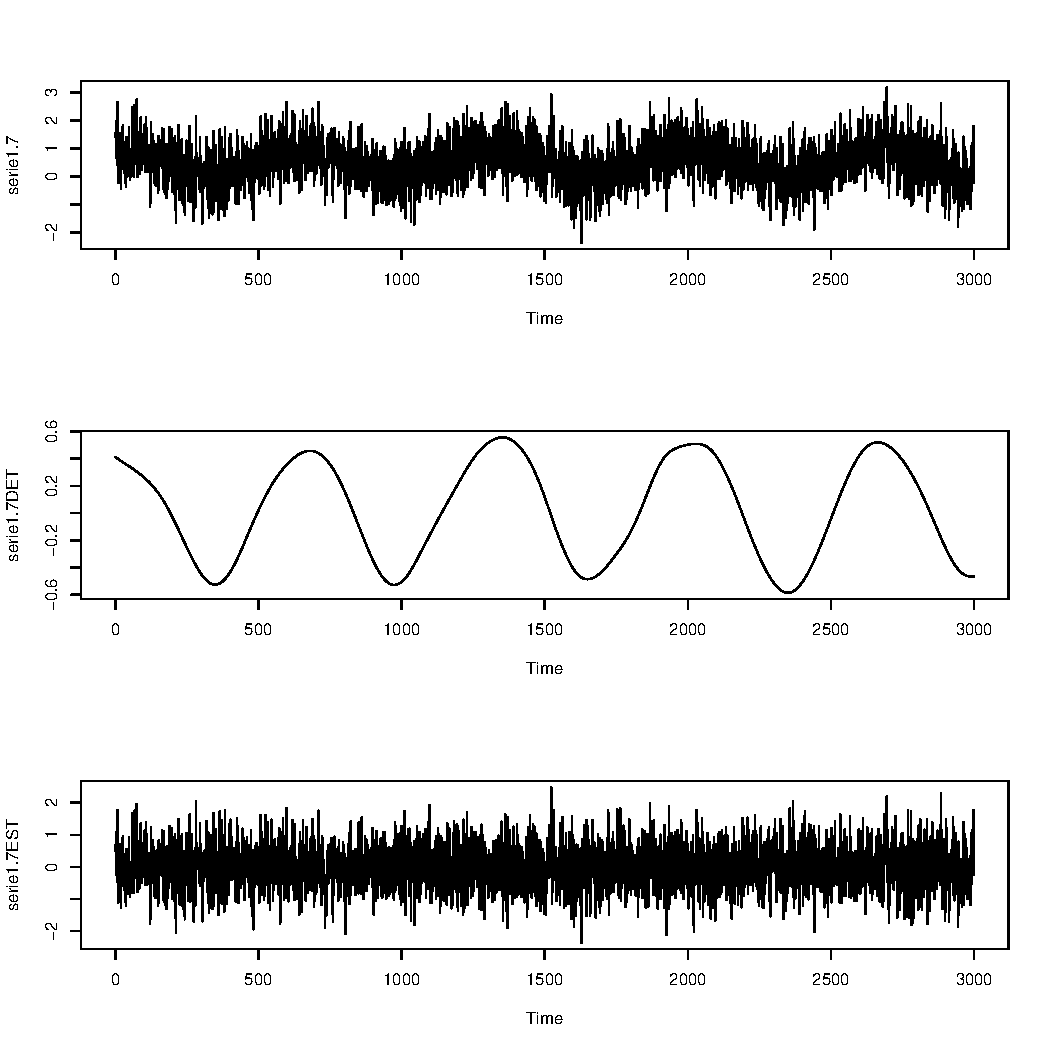
\includegraphics[scale=0.43]{serie1_7.pdf} \quad
  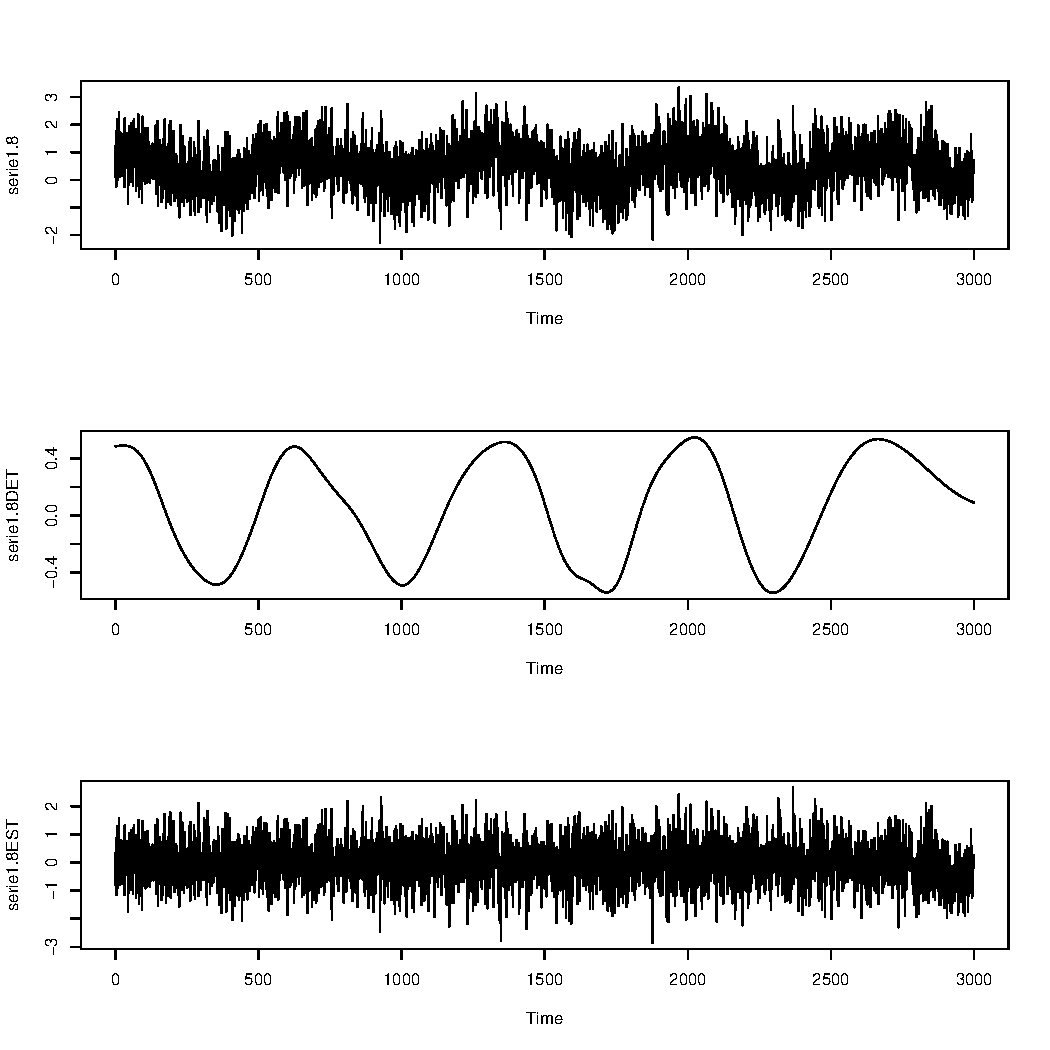
\includegraphics[scale=0.43]{serie1_8.pdf}
  \caption{Série 1.7 e Série 1.8}

\end{center}
\end{figure}

\graphicspath{{imagens/}}
\begin{figure}[H]
\begin{center}
  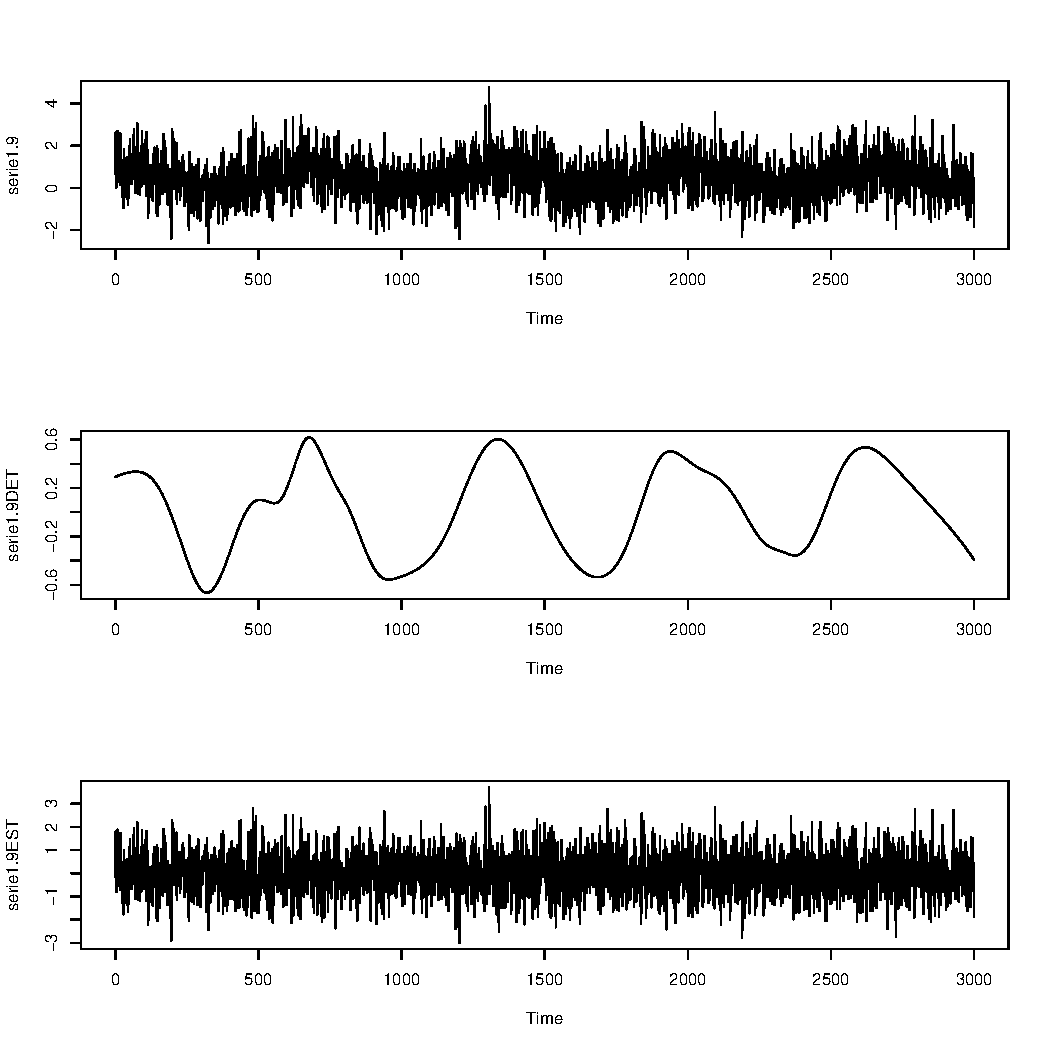
\includegraphics[scale=0.43]{serie1_9.pdf} \quad
  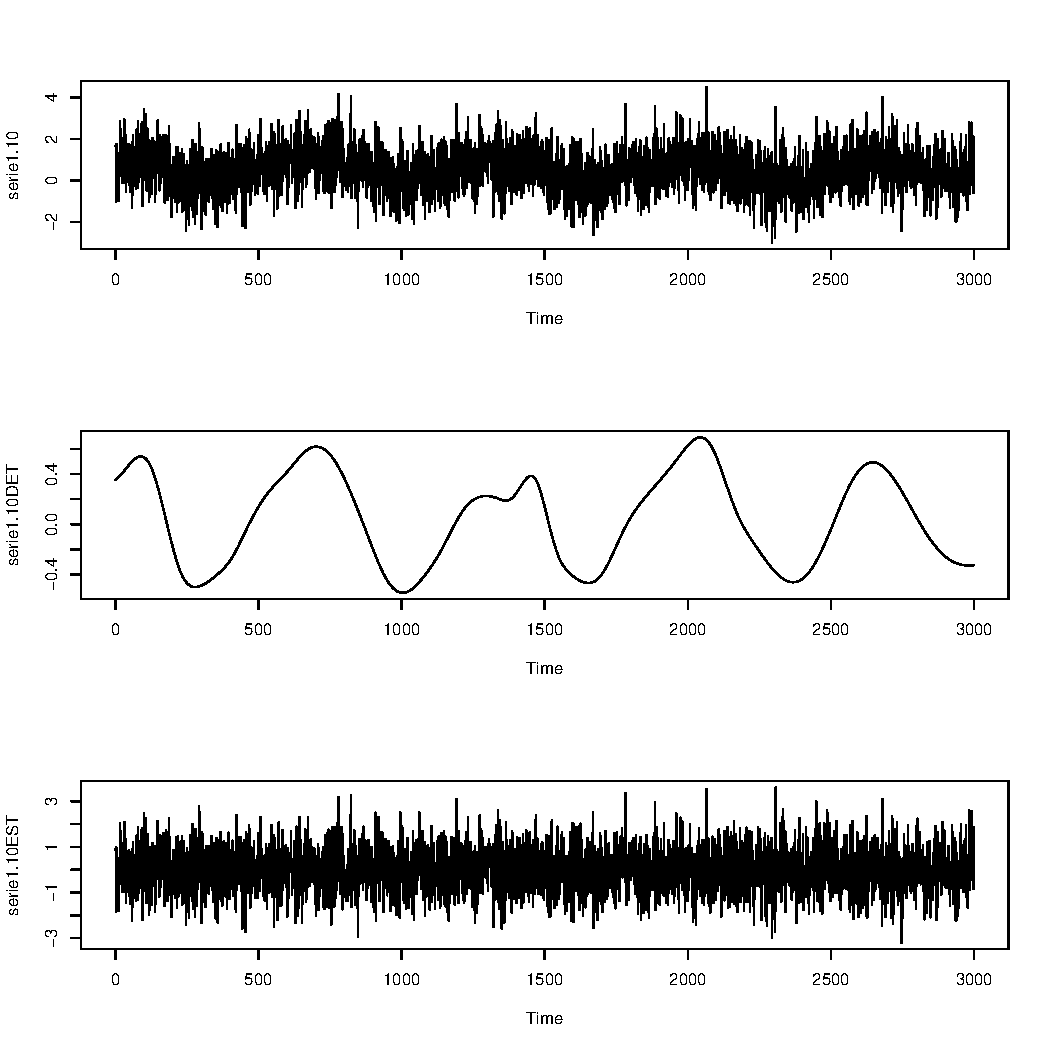
\includegraphics[scale=0.43]{serie1_10.pdf}
  \caption{Série 1.9 e Série 1.10}

\end{center}
\end{figure}

\section{Séries TIPO 2}
10 séries cossenoide com ruído ao longo da série e tendência.
\graphicspath{{imagens/}}
\begin{figure}[H]
\begin{center}
  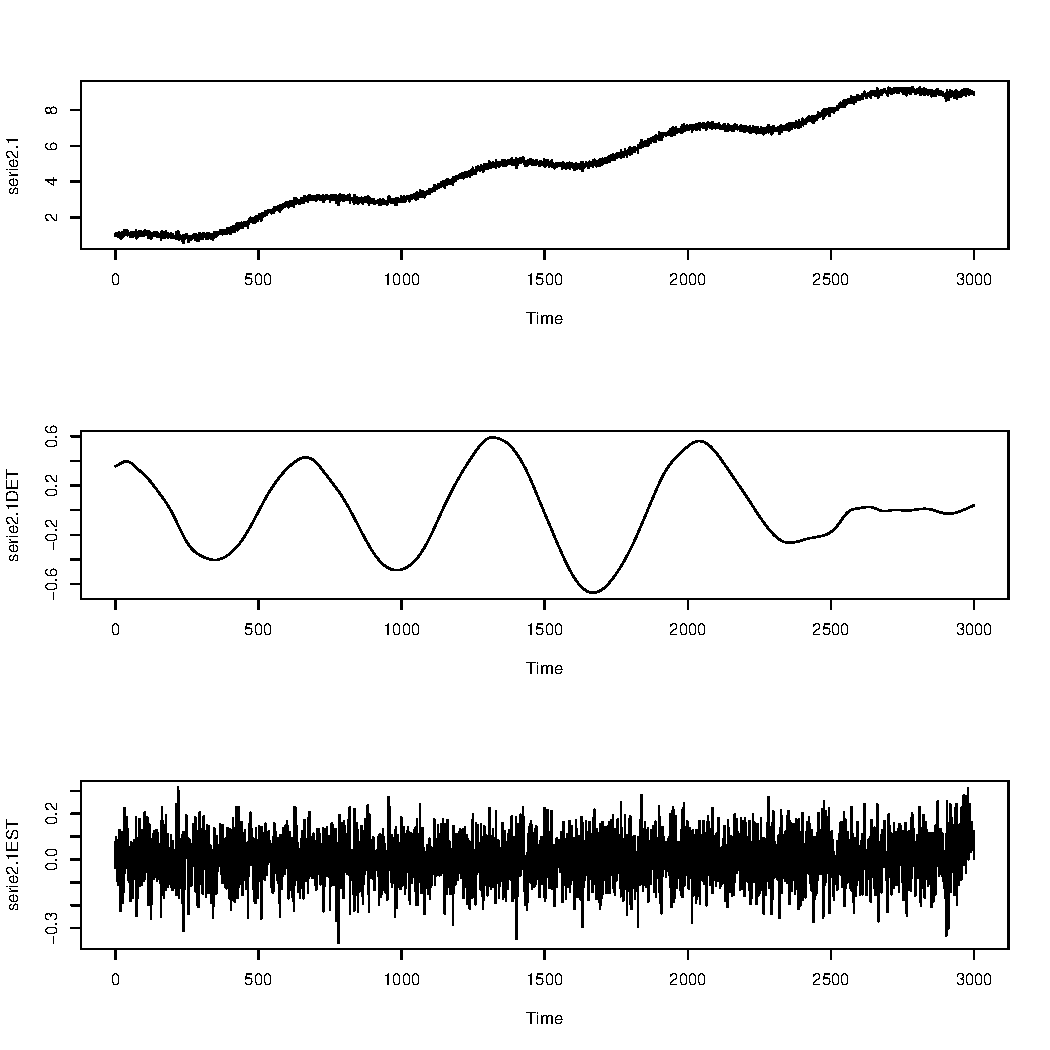
\includegraphics[scale=0.43]{serie2_1.pdf} \quad
  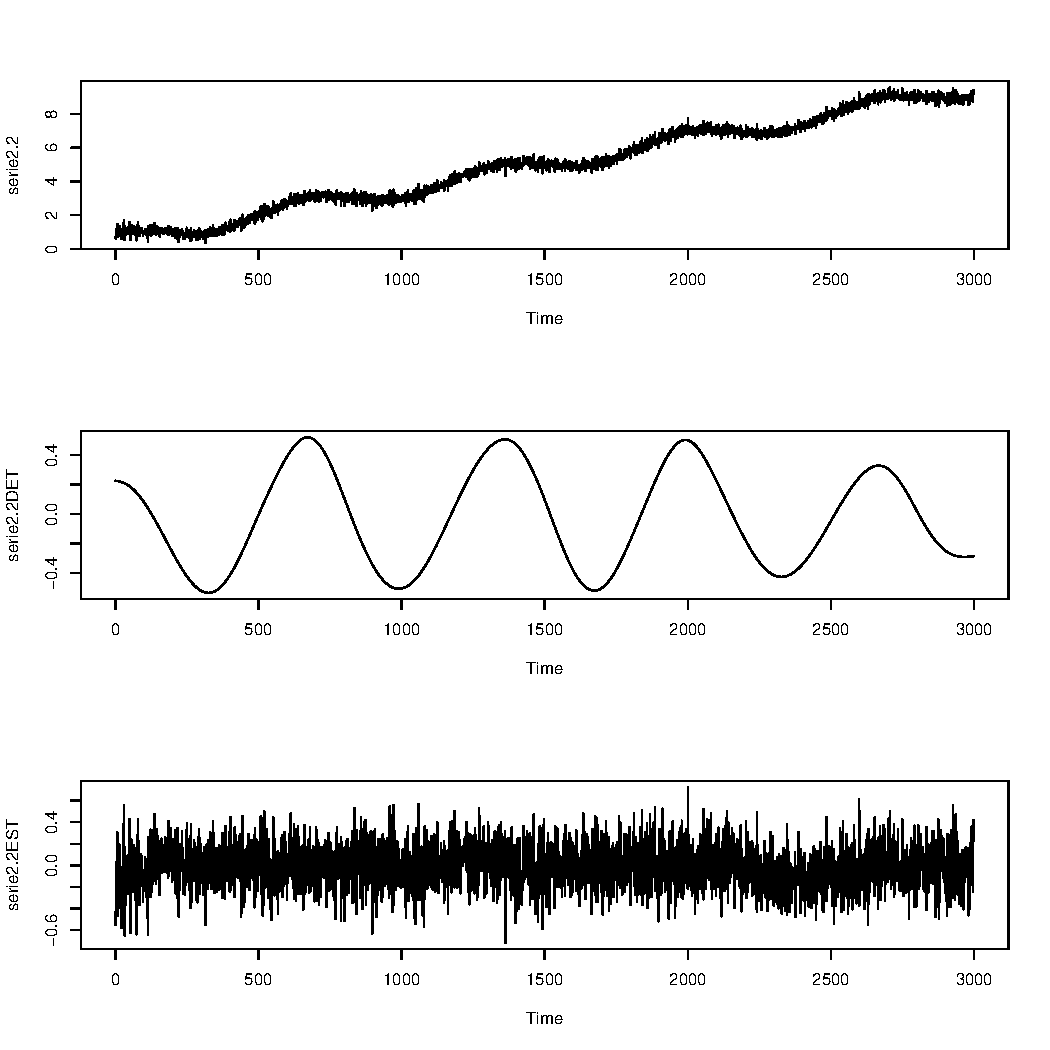
\includegraphics[scale=0.43]{serie2_2.pdf}
  \caption{Série 2.1 e Série 2.2}

\end{center}
\end{figure}

\graphicspath{{imagens/}}
\begin{figure}[H]
\begin{center}
  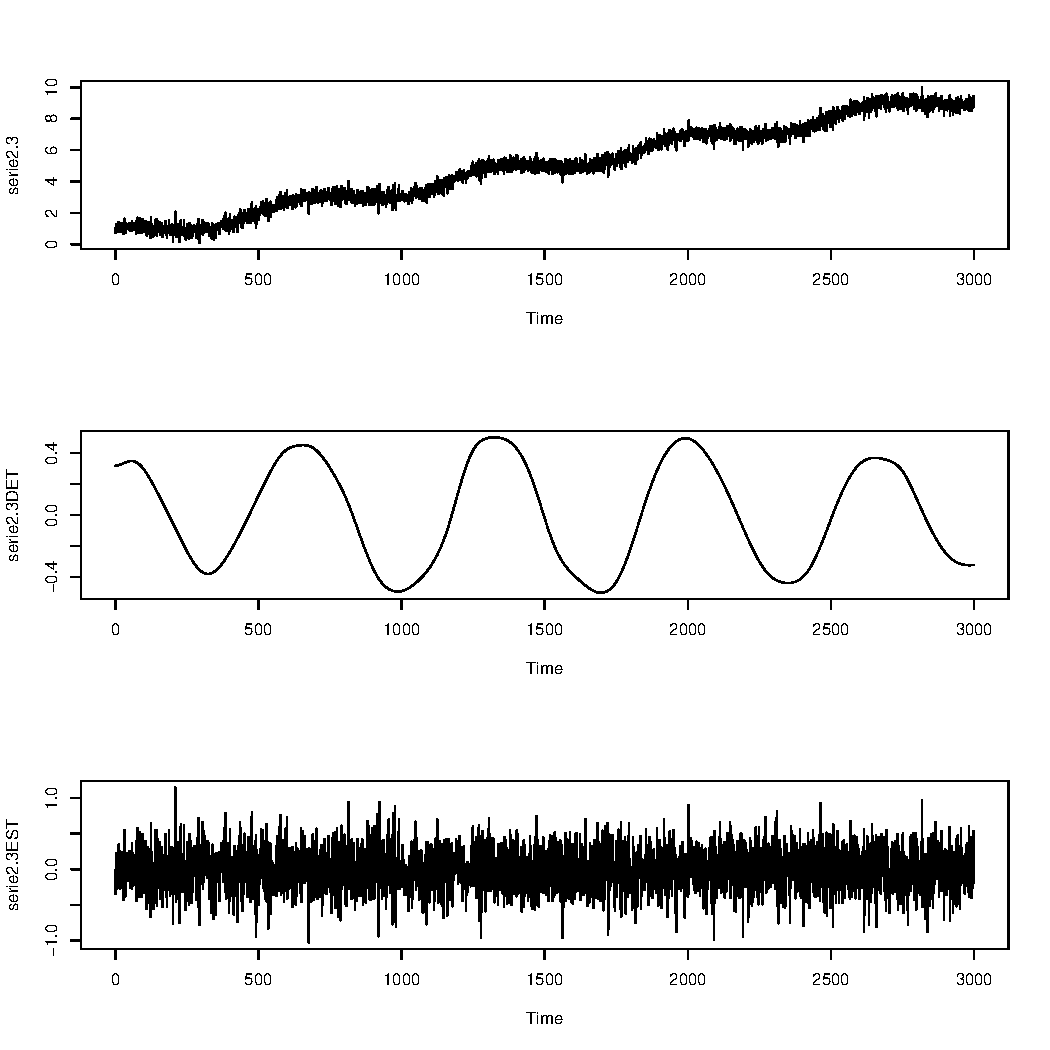
\includegraphics[scale=0.43]{serie2_3.pdf} \quad
  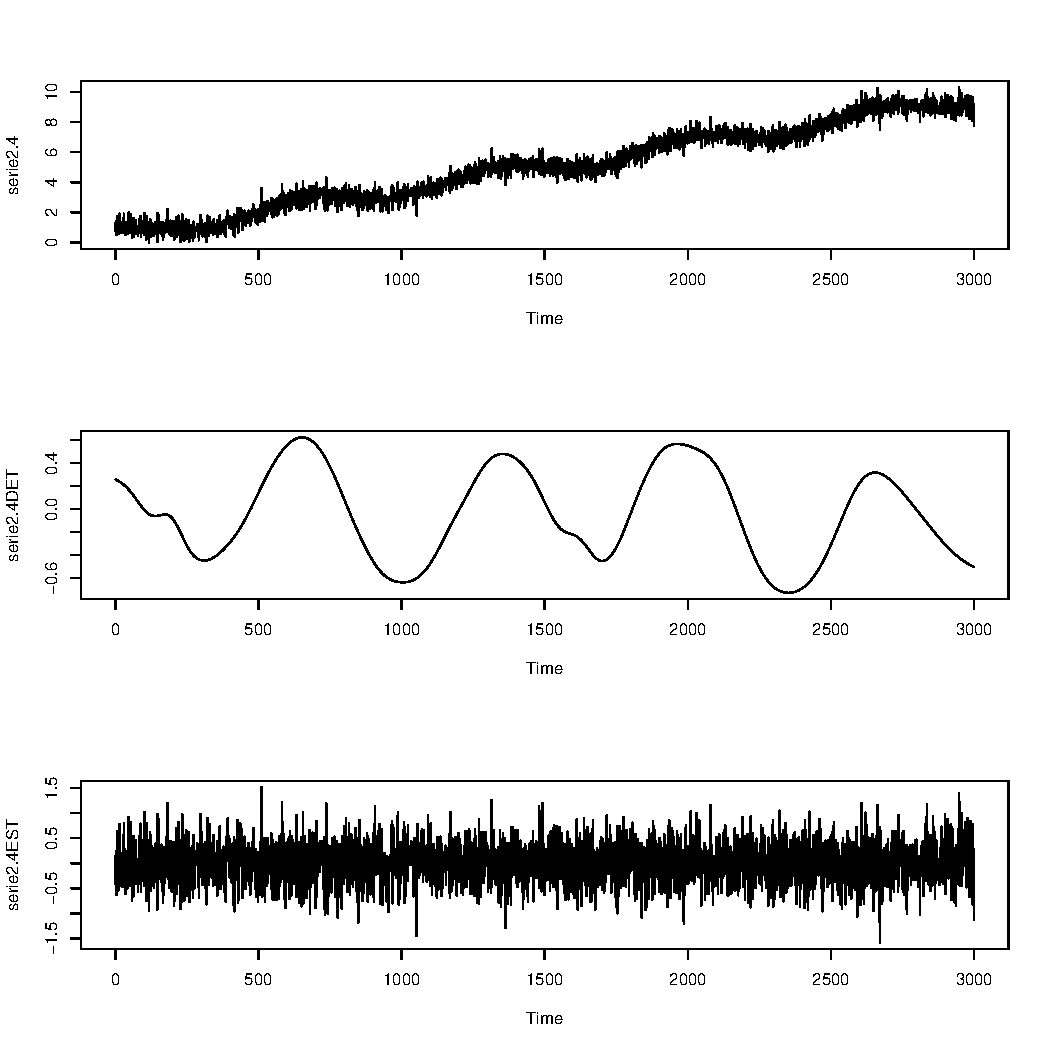
\includegraphics[scale=0.43]{serie2_4.pdf}
  \caption{Série 2.3 e Série 2.4}

\end{center}
\end{figure}

\graphicspath{{imagens/}}
\begin{figure}[H]
\begin{center}
  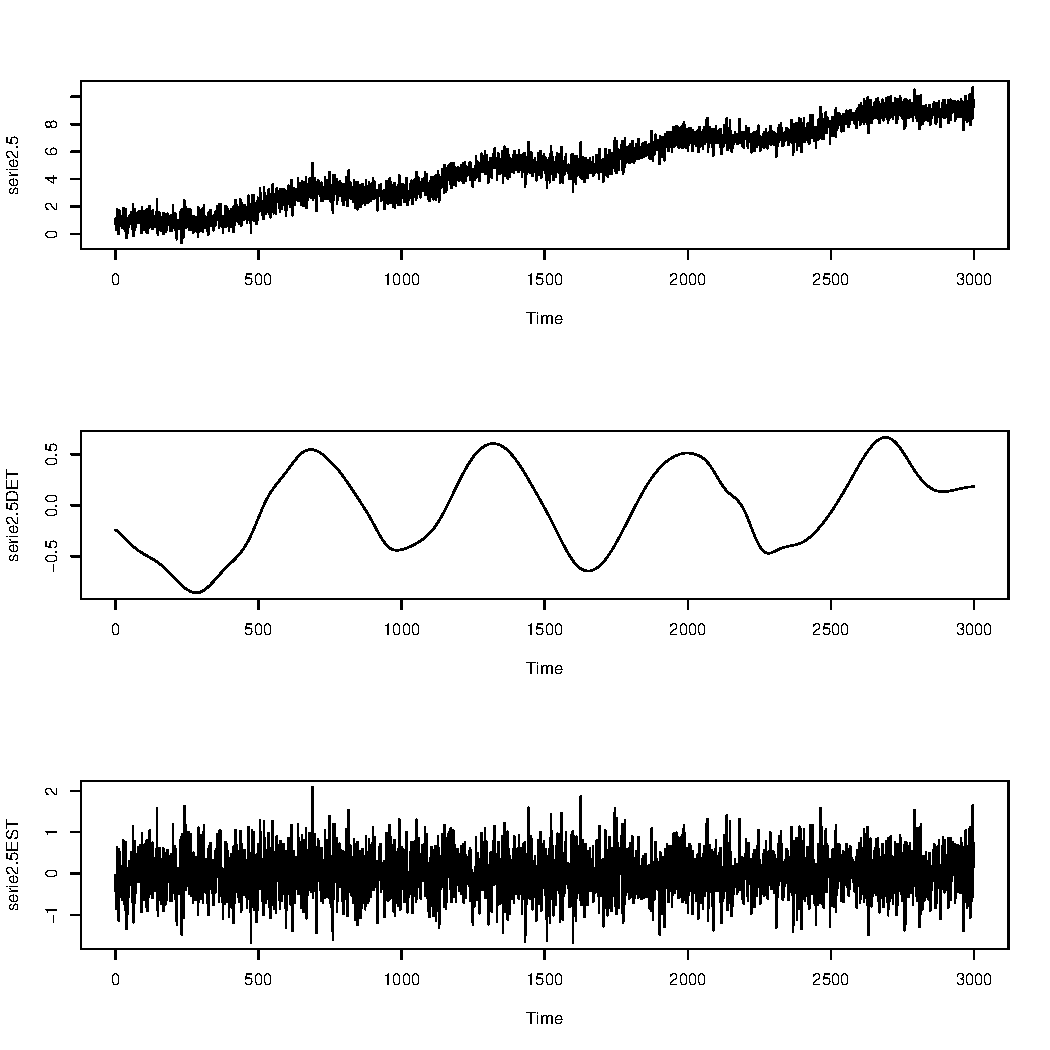
\includegraphics[scale=0.43]{serie2_5.pdf} \quad
  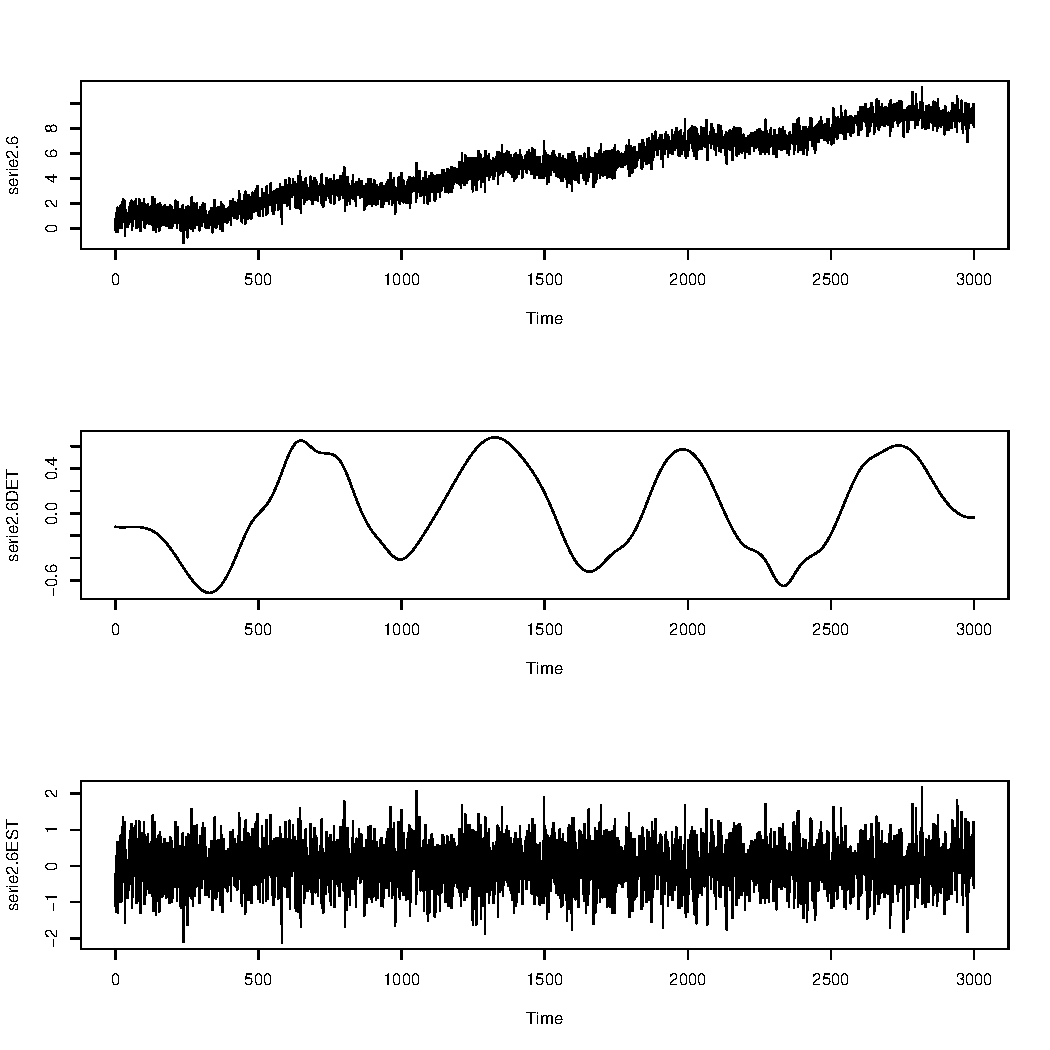
\includegraphics[scale=0.43]{serie2_6.pdf}
  \caption{Série 2.5 e Série 2.6}

\end{center}
\end{figure}

\graphicspath{{imagens/}}
\begin{figure}[H]
\begin{center}
  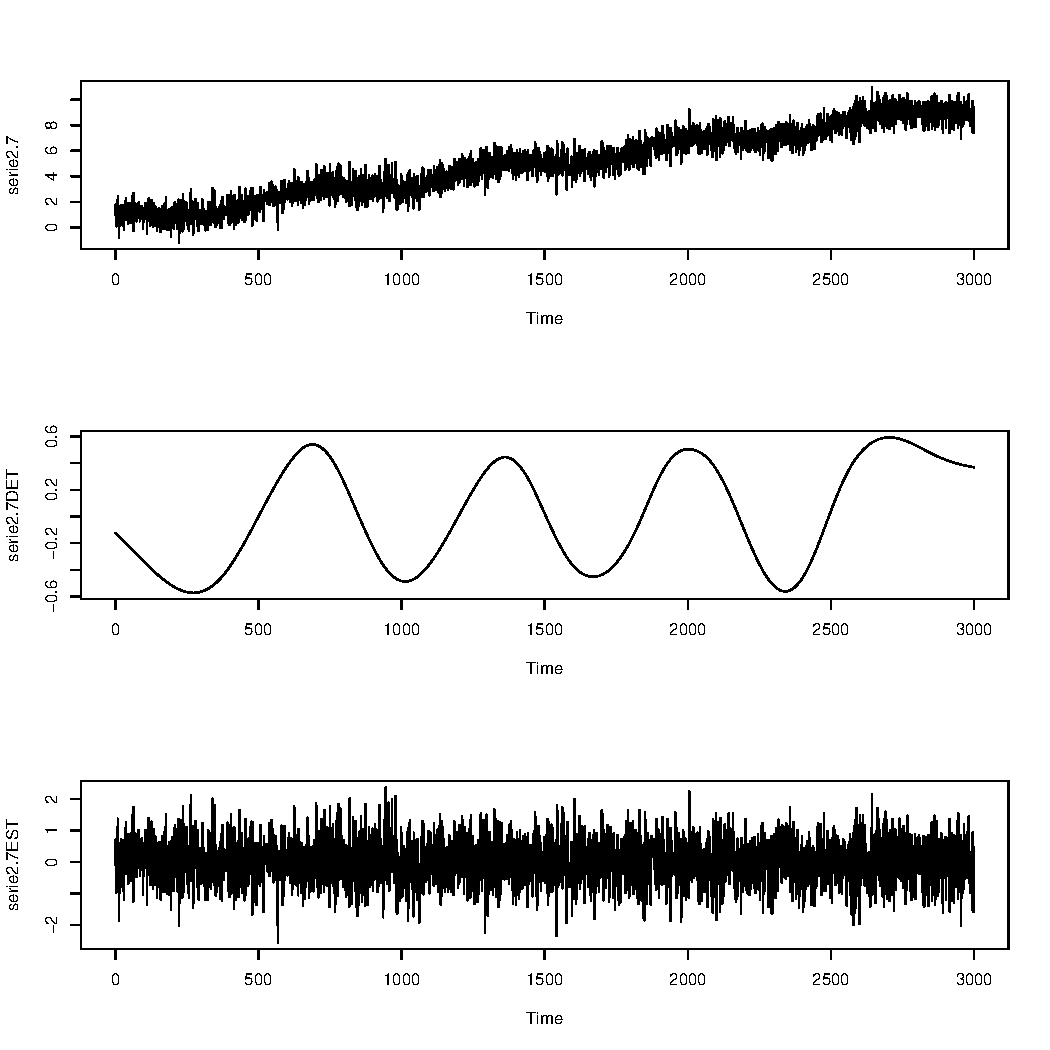
\includegraphics[scale=0.43]{serie2_7.pdf} \quad
  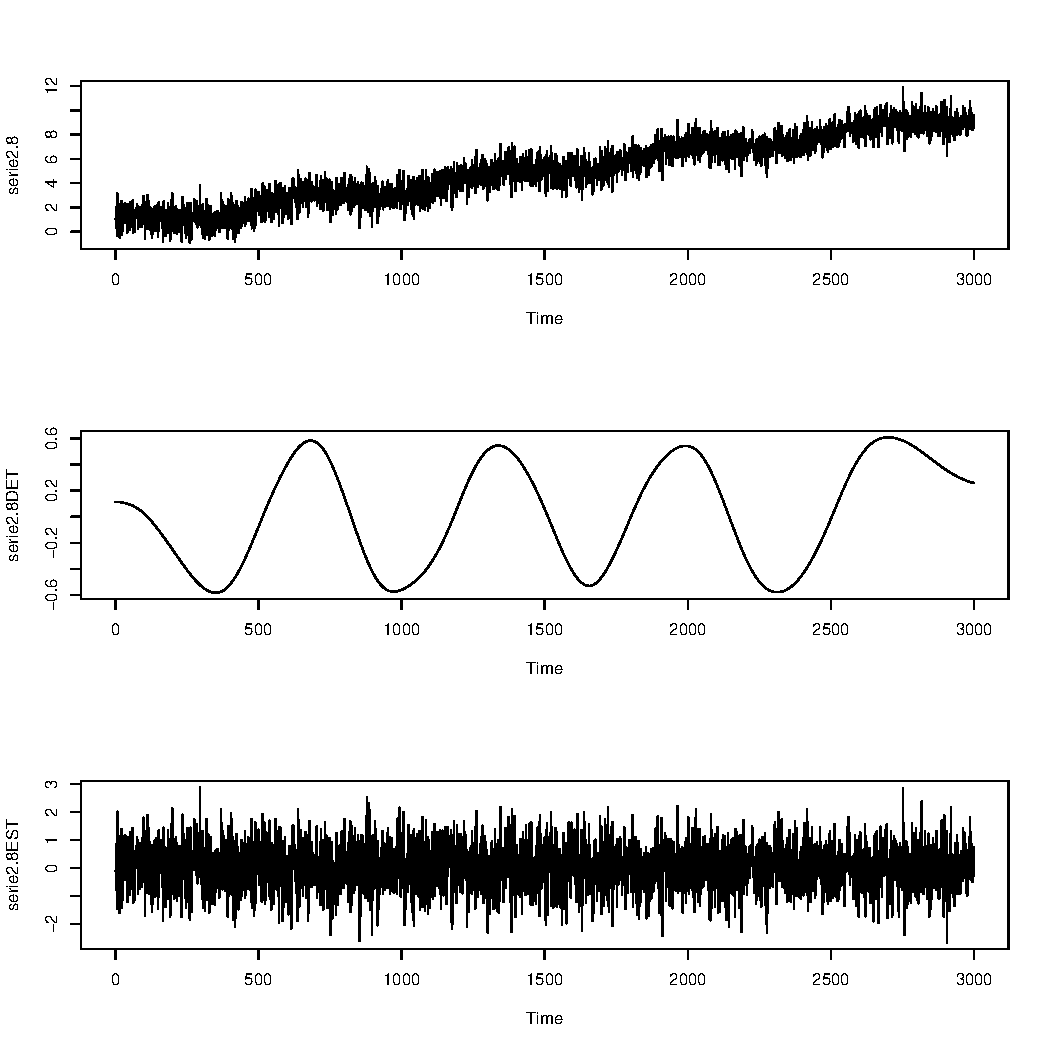
\includegraphics[scale=0.43]{serie2_8.pdf}
  \caption{Série 2.7 e Série 2.8}

\end{center}
\end{figure}

\graphicspath{{imagens/}}
\begin{figure}[H]
\begin{center}
  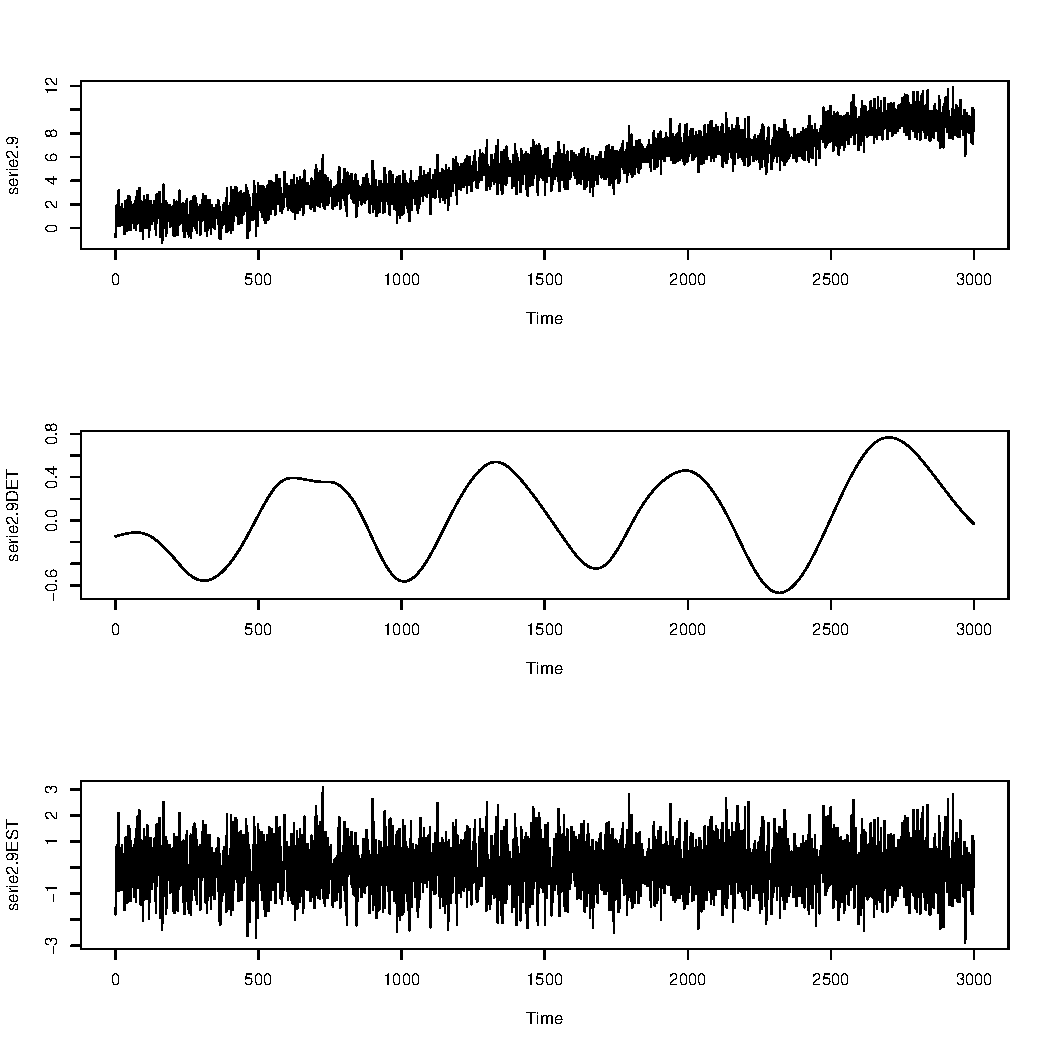
\includegraphics[scale=0.43]{serie2_9.pdf} \quad
  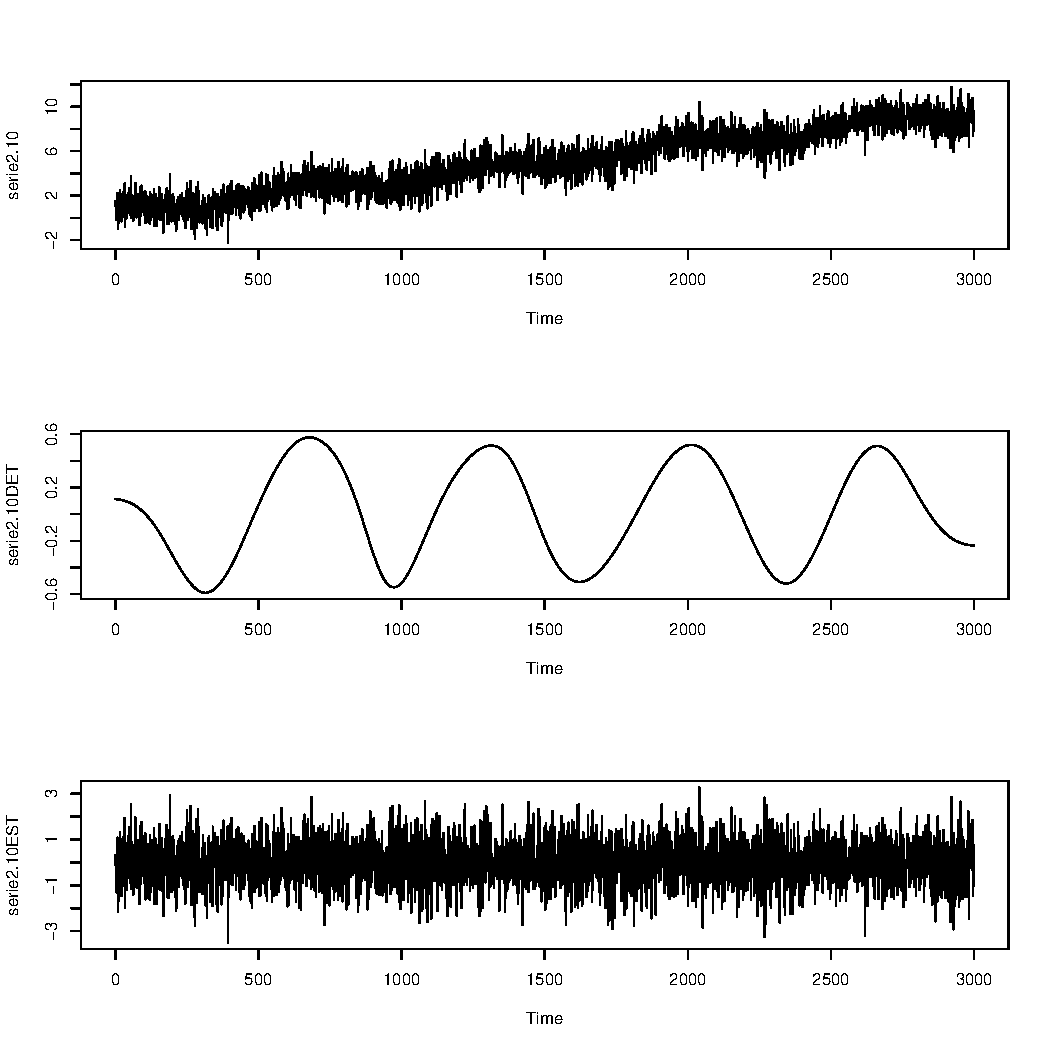
\includegraphics[scale=0.43]{serie2_10.pdf}
  \caption{Série 2.9 e Série 2.10}

\end{center}
\end{figure}

\section{Séries TIPO 3}
10 séries senoide com ruído ao longo da série.
\graphicspath{{imagens/}}
\begin{figure}[H]
\begin{center}
  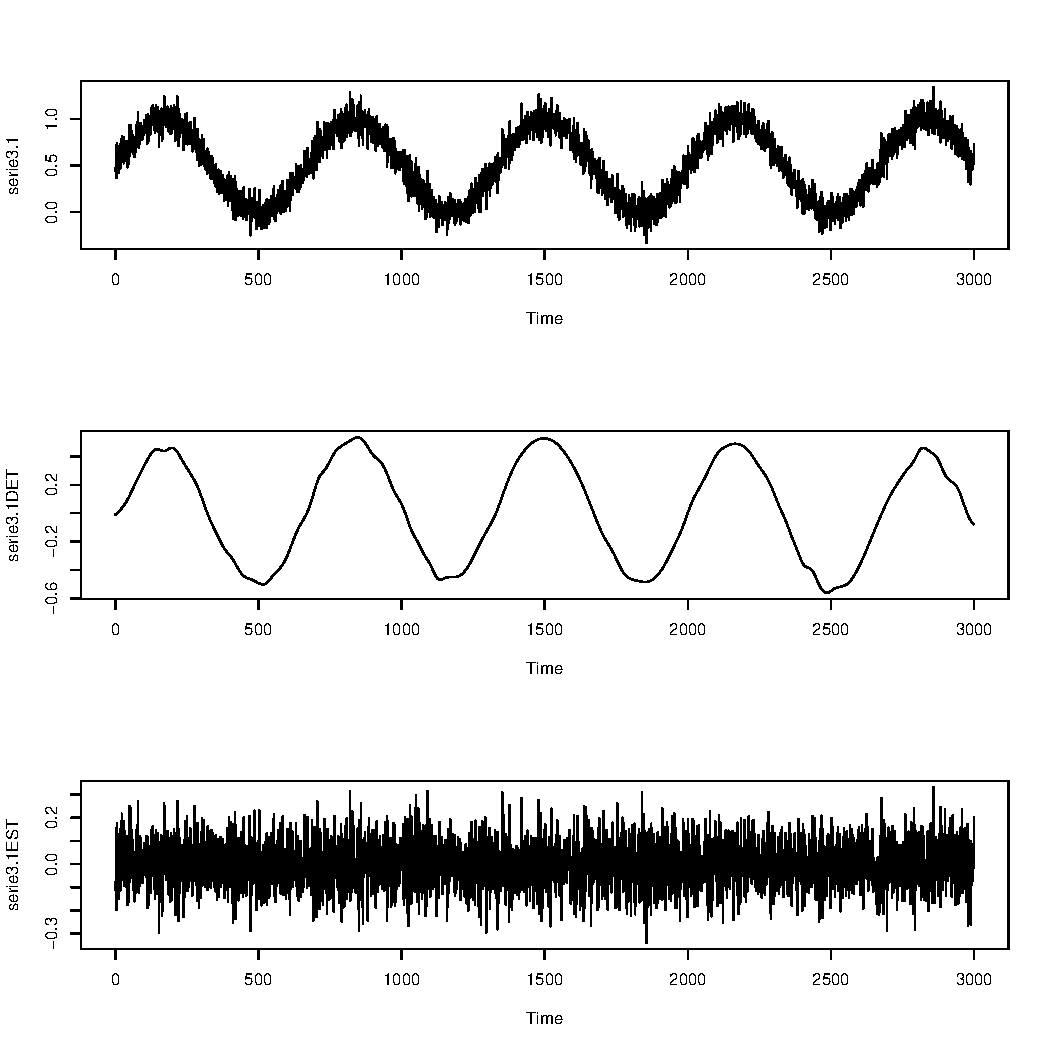
\includegraphics[scale=0.43]{serie3_1.pdf} \quad
  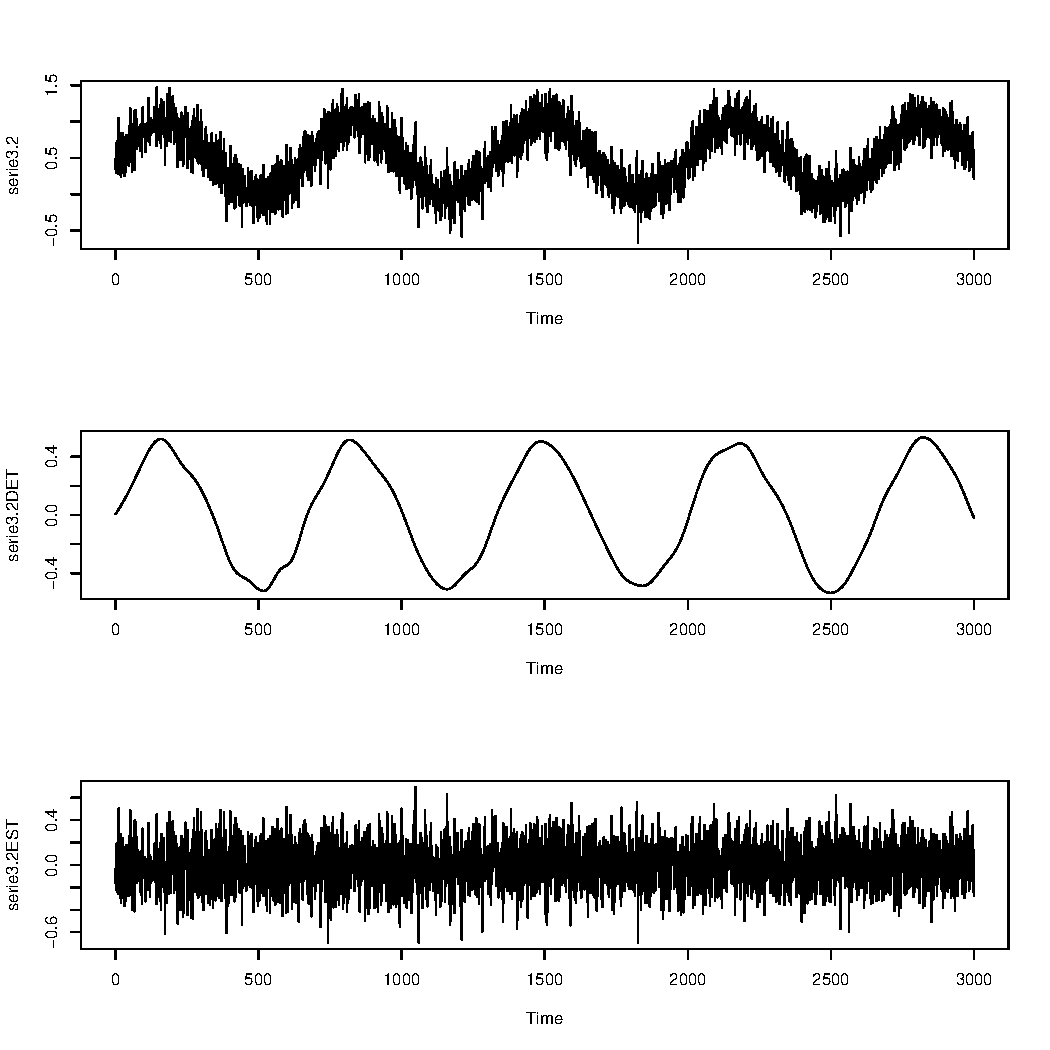
\includegraphics[scale=0.43]{serie3_2.pdf}
  \caption{Série 3.1 e Série 3.2}

\end{center}
\end{figure}

\graphicspath{{imagens/}}
\begin{figure}[H]
\begin{center}
  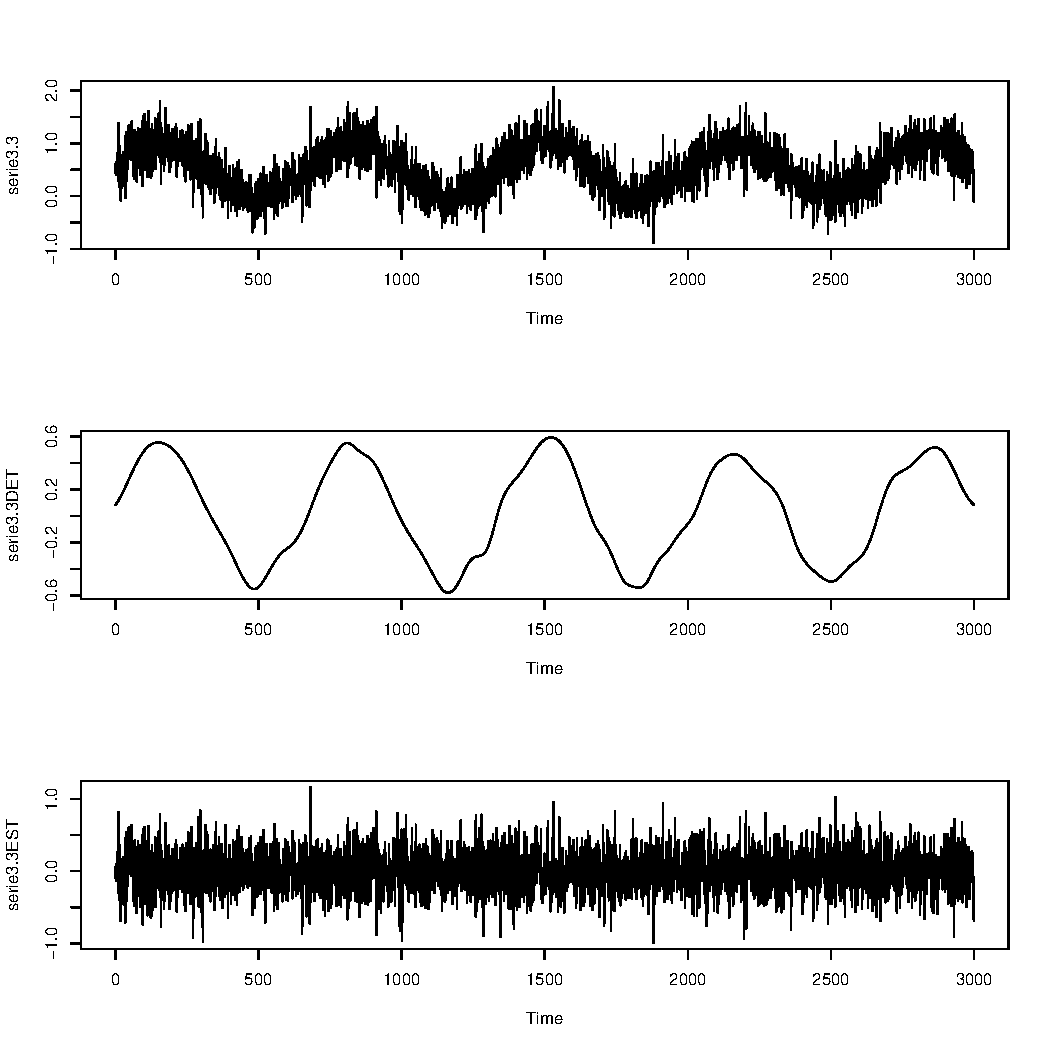
\includegraphics[scale=0.43]{serie3_3.pdf} \quad
  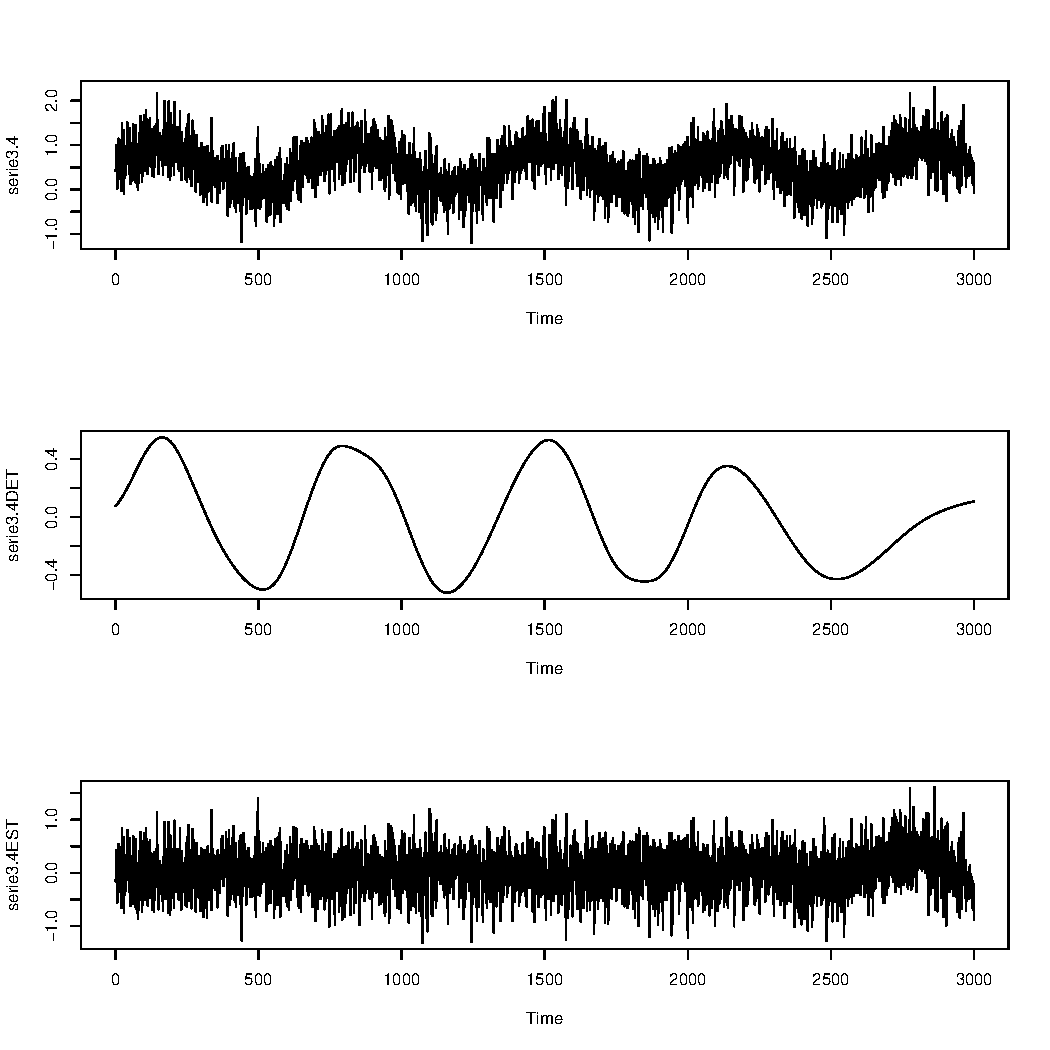
\includegraphics[scale=0.43]{serie3_4.pdf}
  \caption{Série 3.3 e Série 3.4}

\end{center}
\end{figure}

\graphicspath{{imagens/}}
\begin{figure}[H]
\begin{center}
  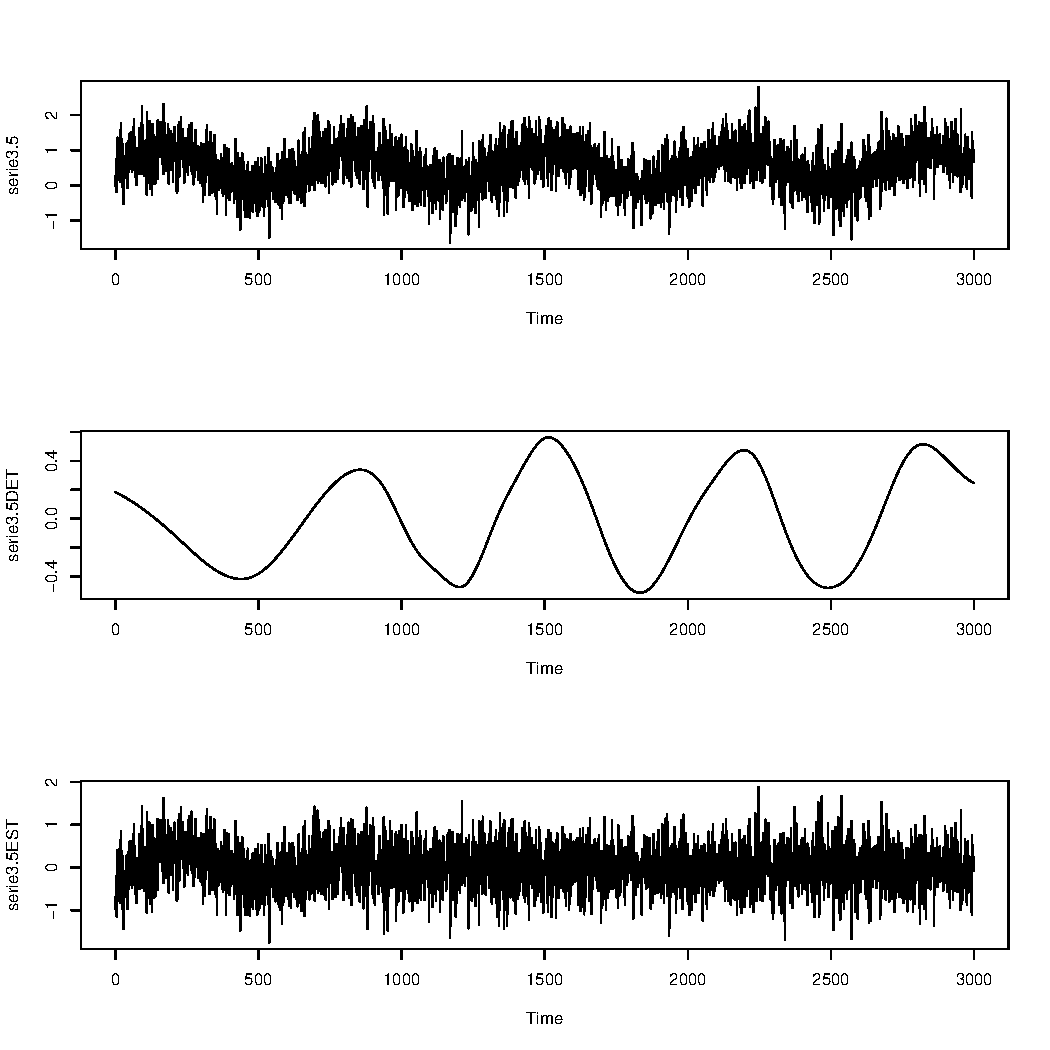
\includegraphics[scale=0.43]{serie3_5.pdf} \quad
  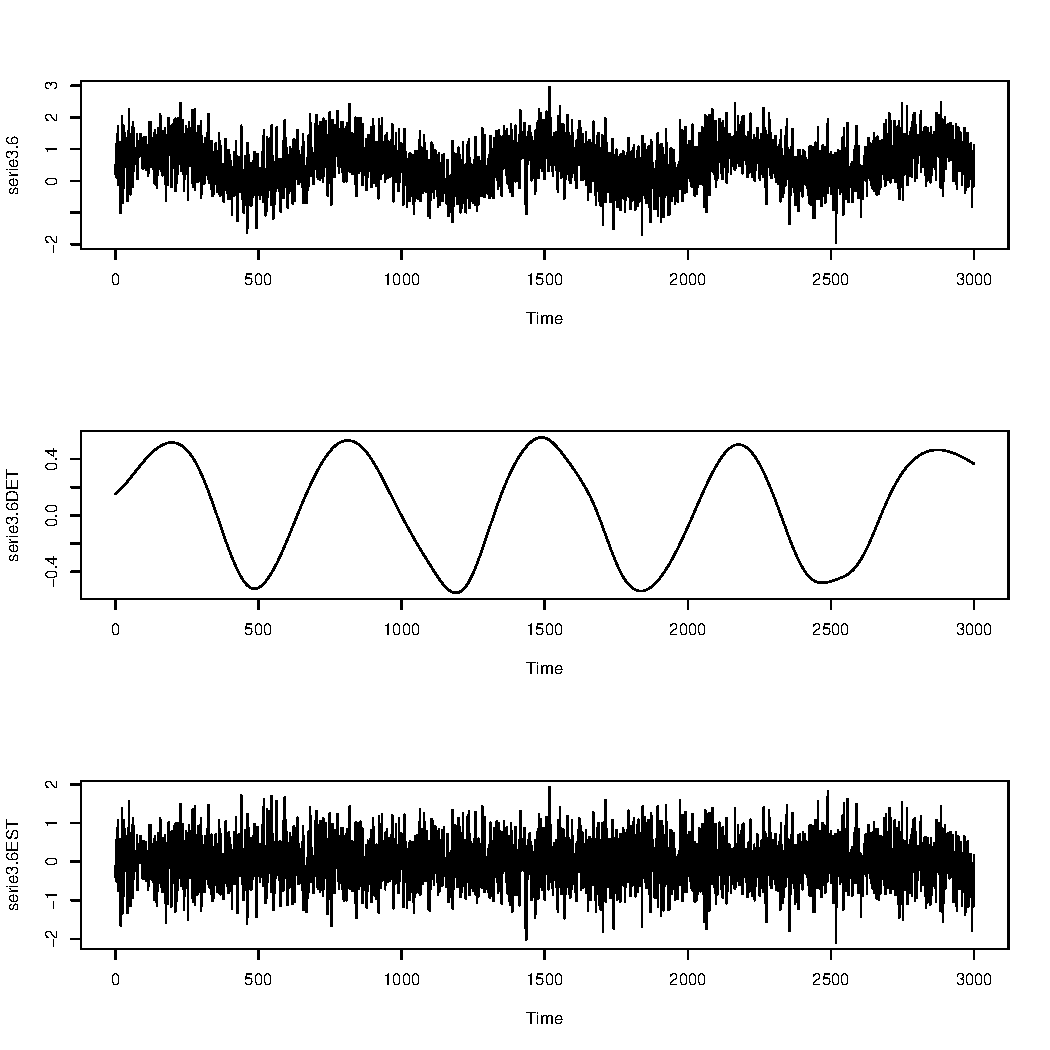
\includegraphics[scale=0.43]{serie3_6.pdf}
  \caption{Série 3.5 e Série 3.6}

\end{center}
\end{figure}

\graphicspath{{imagens/}}
\begin{figure}[H]
\begin{center}
  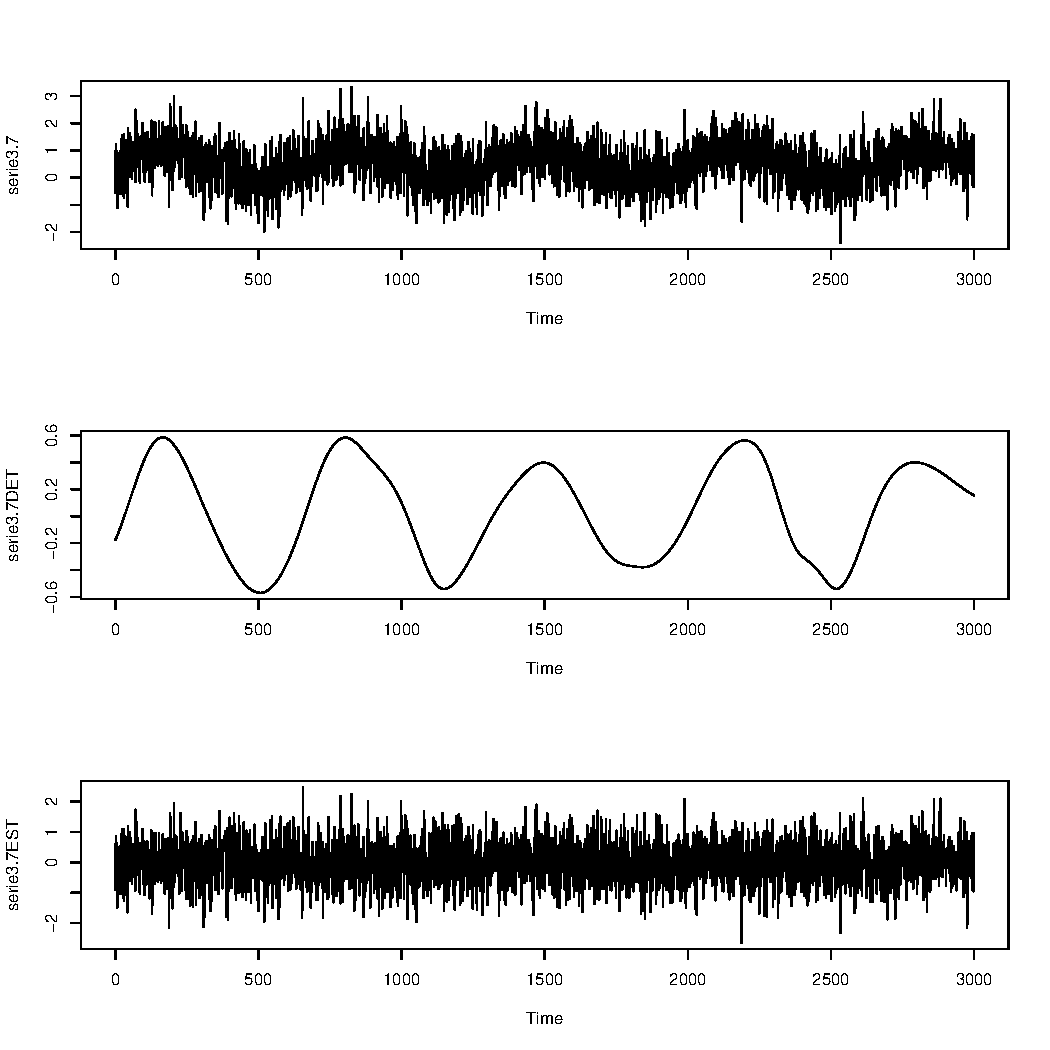
\includegraphics[scale=0.43]{serie3_7.pdf} \quad
  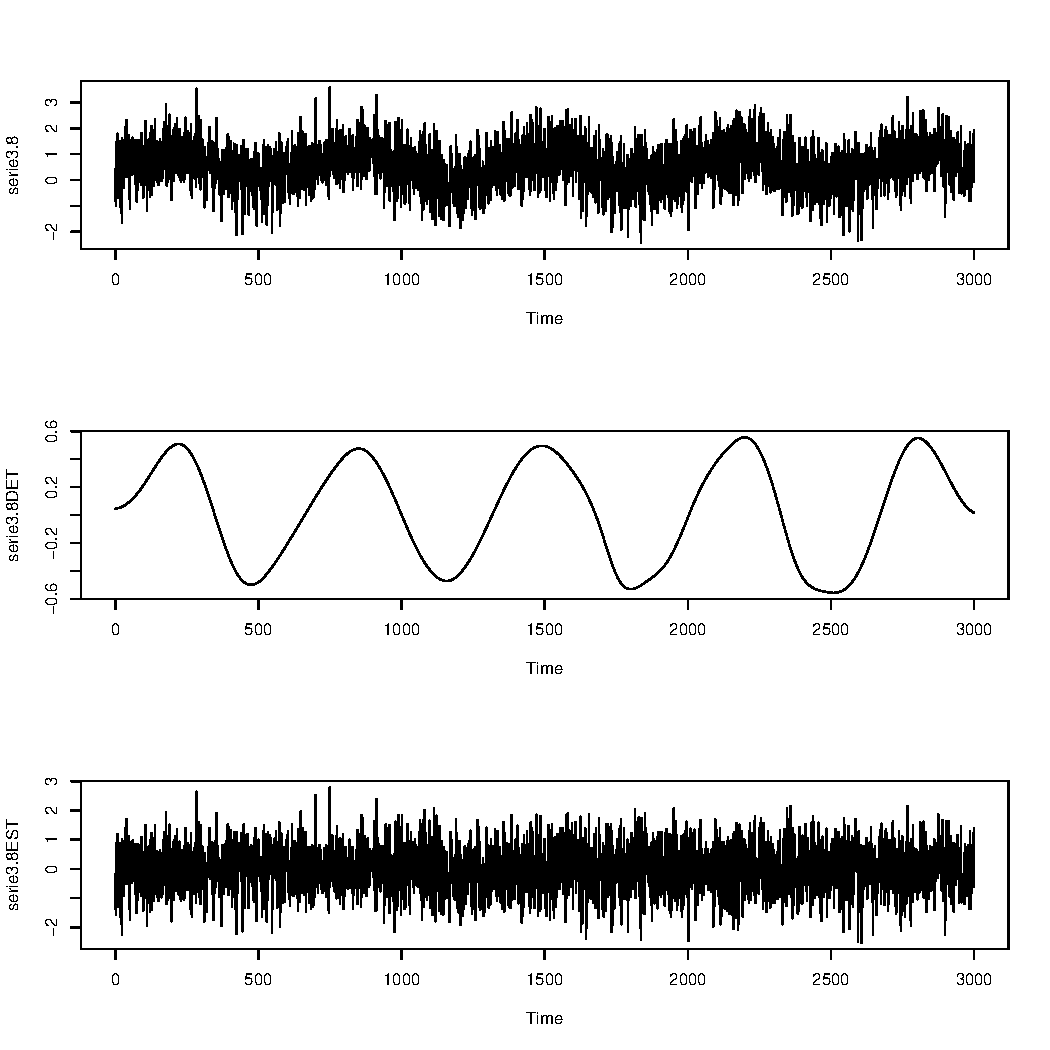
\includegraphics[scale=0.43]{serie3_8.pdf}
  \caption{Série 3.7 e Série 3.8}

\end{center}
\end{figure}

\graphicspath{{imagens/}}
\begin{figure}[H]
\begin{center}
  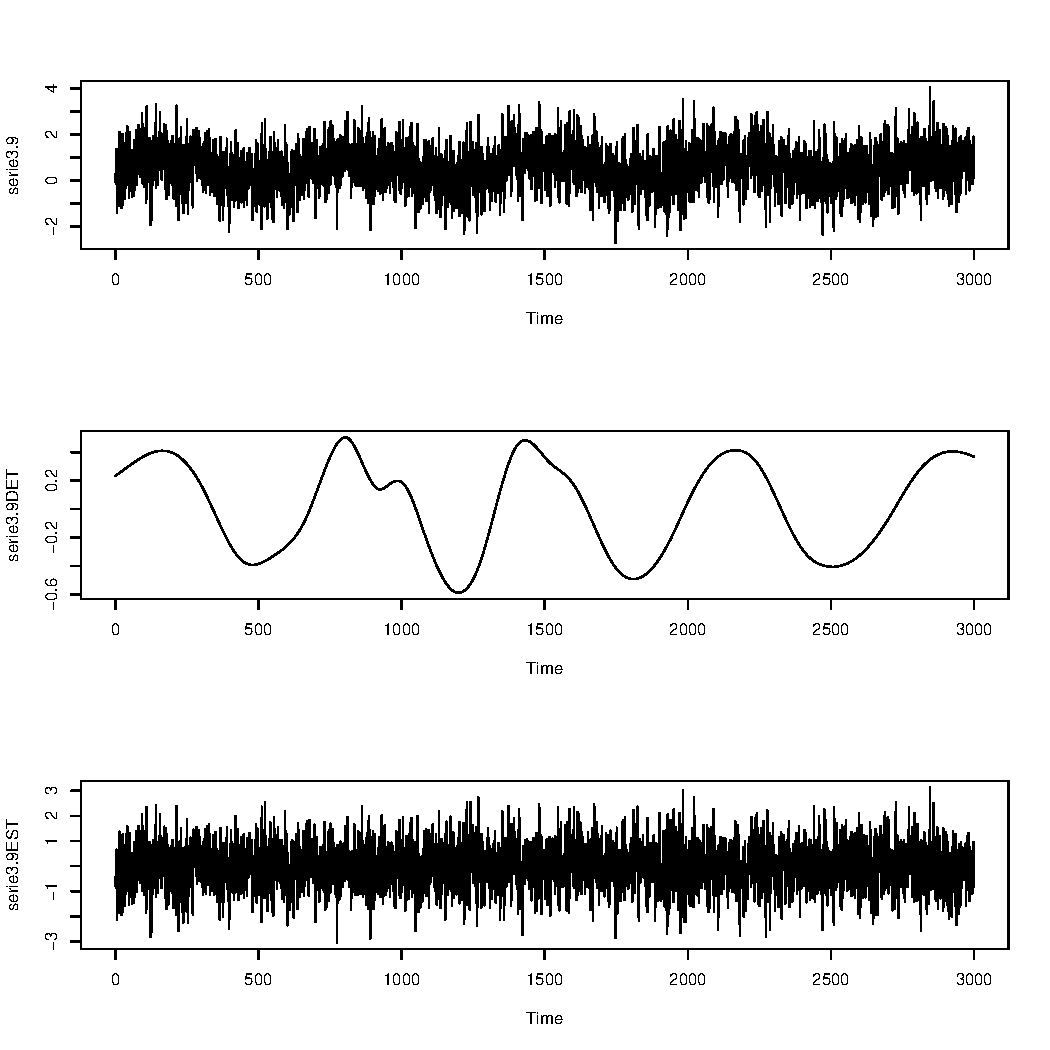
\includegraphics[scale=0.43]{serie3_9.pdf} \quad
  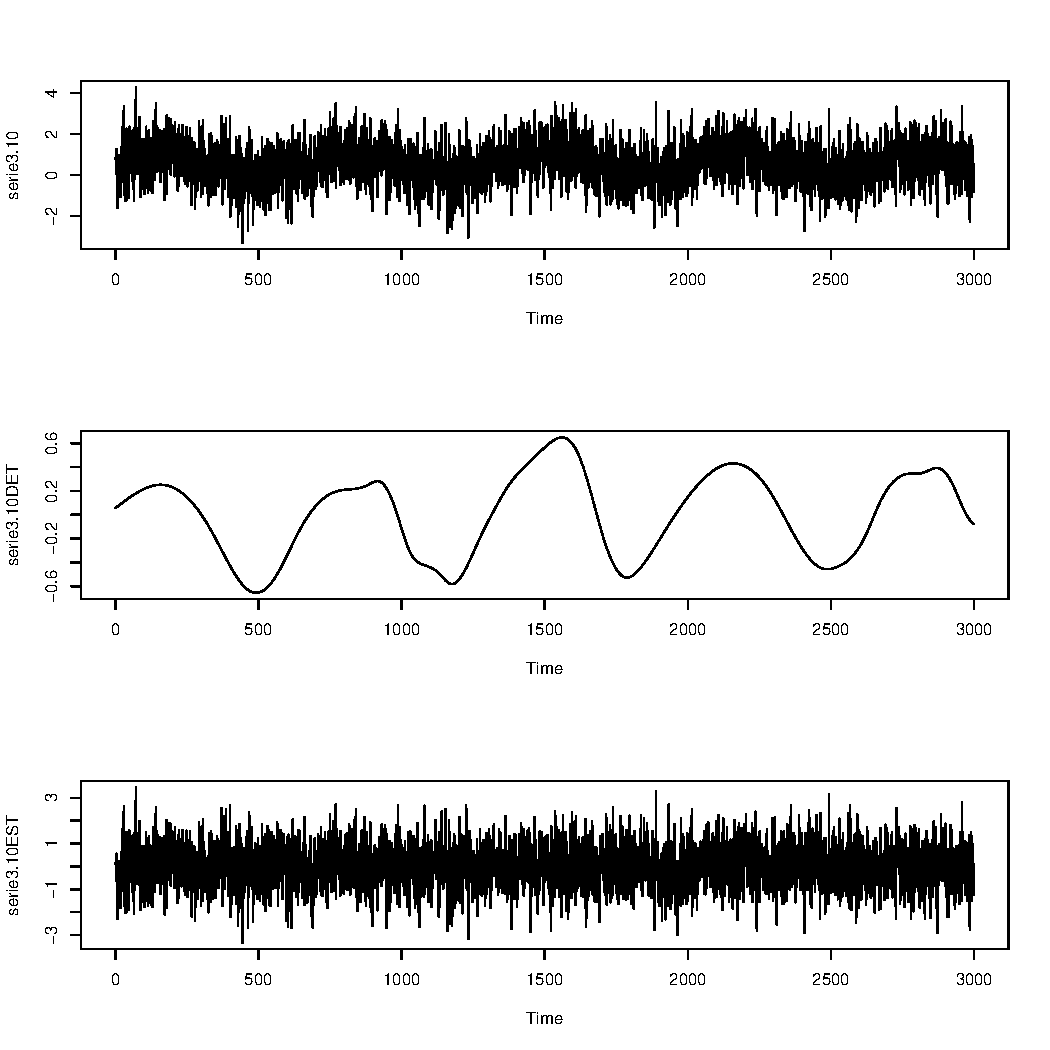
\includegraphics[scale=0.43]{serie3_10.pdf}
  \caption{Série 3.9 e Série 3.10}

\end{center}
\end{figure}

\section{Séries TIPO 4}
10 séries senoide com ruído ao longo da série e tendência.
\graphicspath{{imagens/}}
\begin{figure}[H]
\begin{center}
  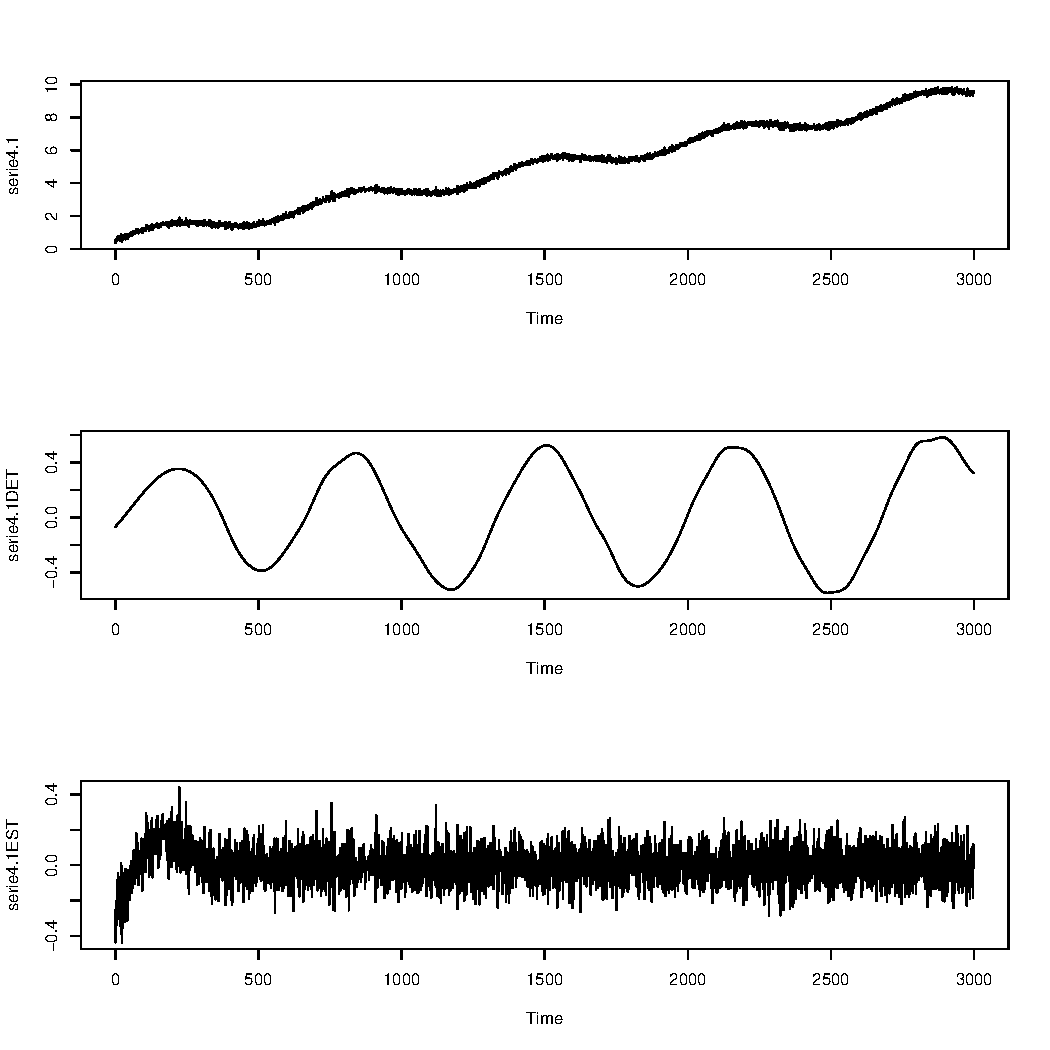
\includegraphics[scale=0.43]{serie4_1.pdf} \quad
  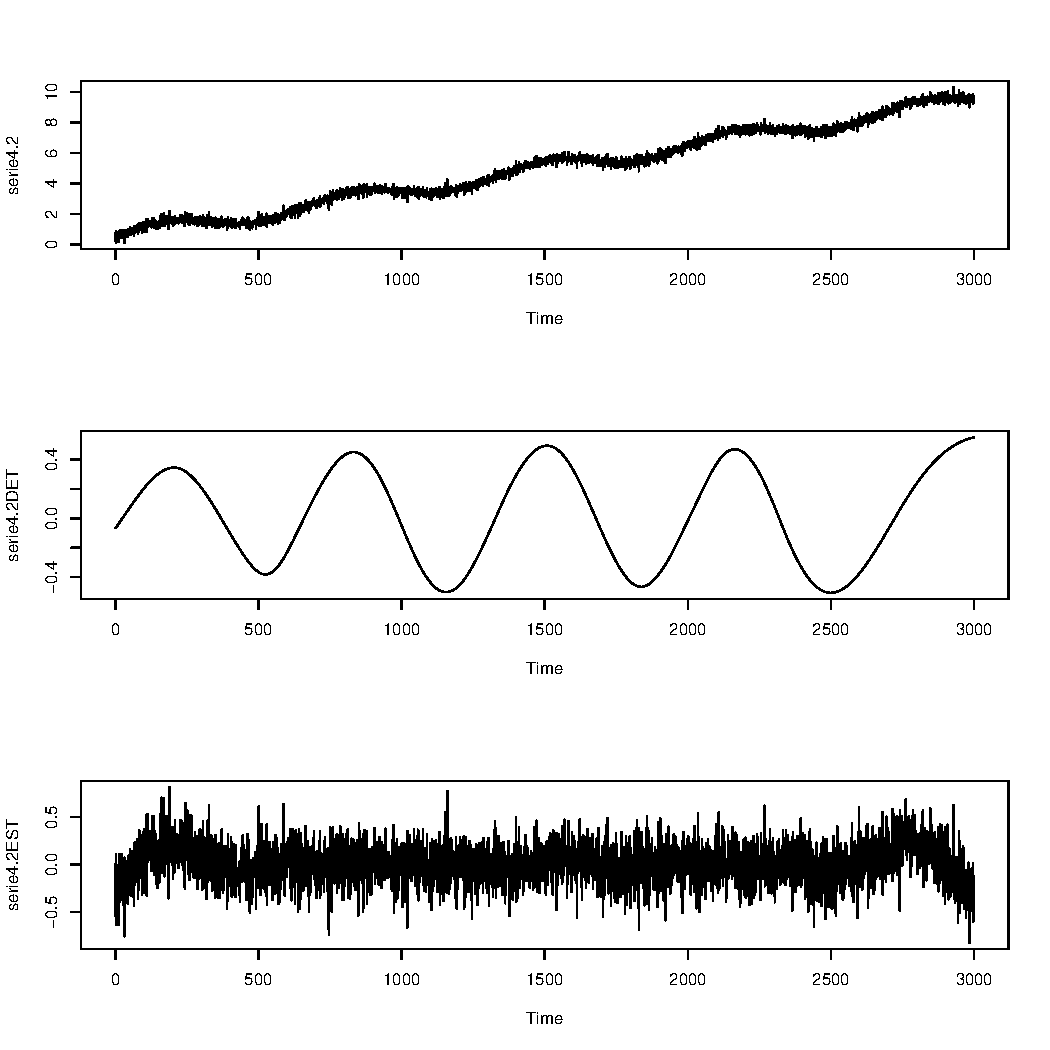
\includegraphics[scale=0.43]{serie4_2.pdf}
  \caption{Série 4.1 e Série 4.2}
\end{center}
\end{figure}

\graphicspath{{imagens/}}
\begin{figure}[H]
\begin{center}
  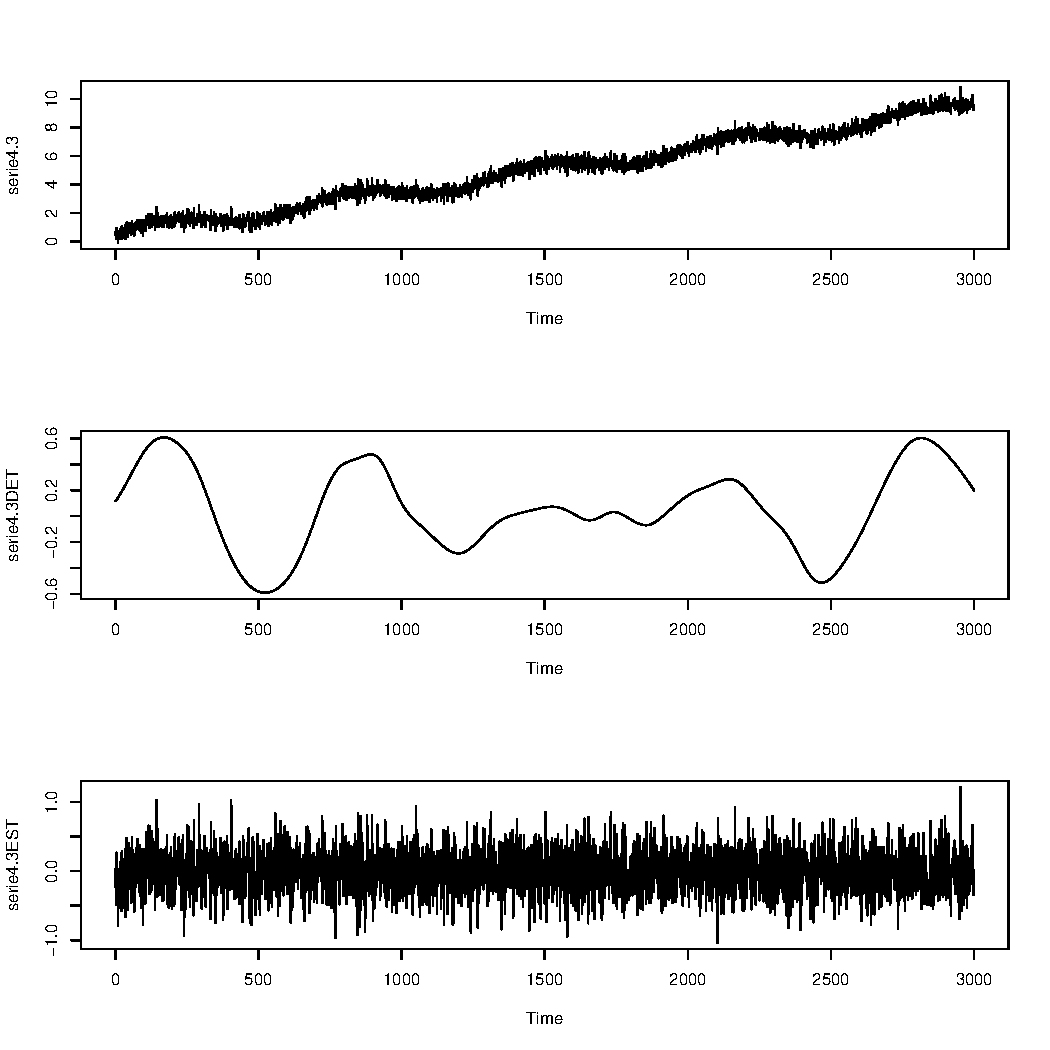
\includegraphics[scale=0.43]{serie4_3.pdf} \quad
 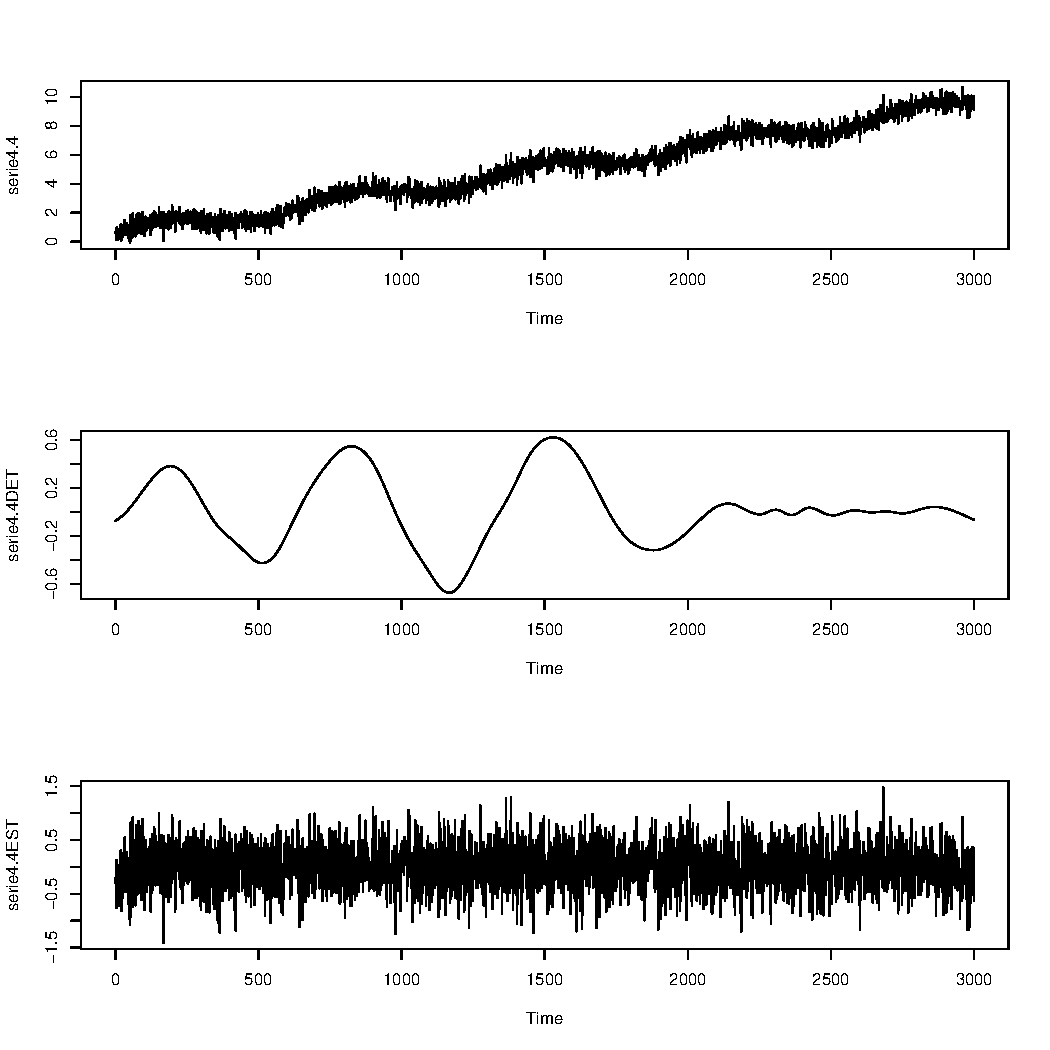
\includegraphics[scale=0.43]{serie4_4.pdf}
 \caption{Série 4.3 e Série 4.4}

\end{center}
\end{figure}

\graphicspath{{imagens/}}
\begin{figure}[H]
\begin{center}
  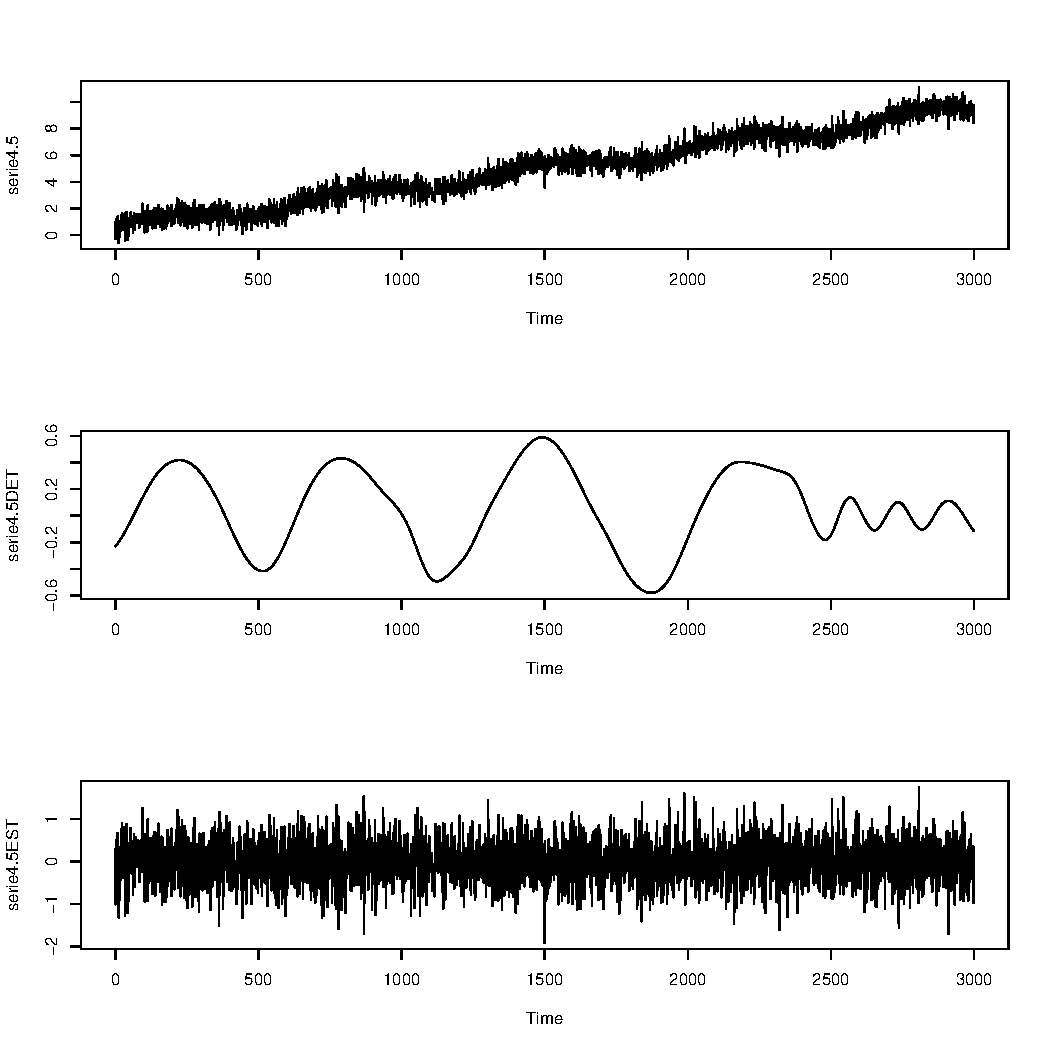
\includegraphics[scale=0.43]{serie4_5.pdf} \quad
  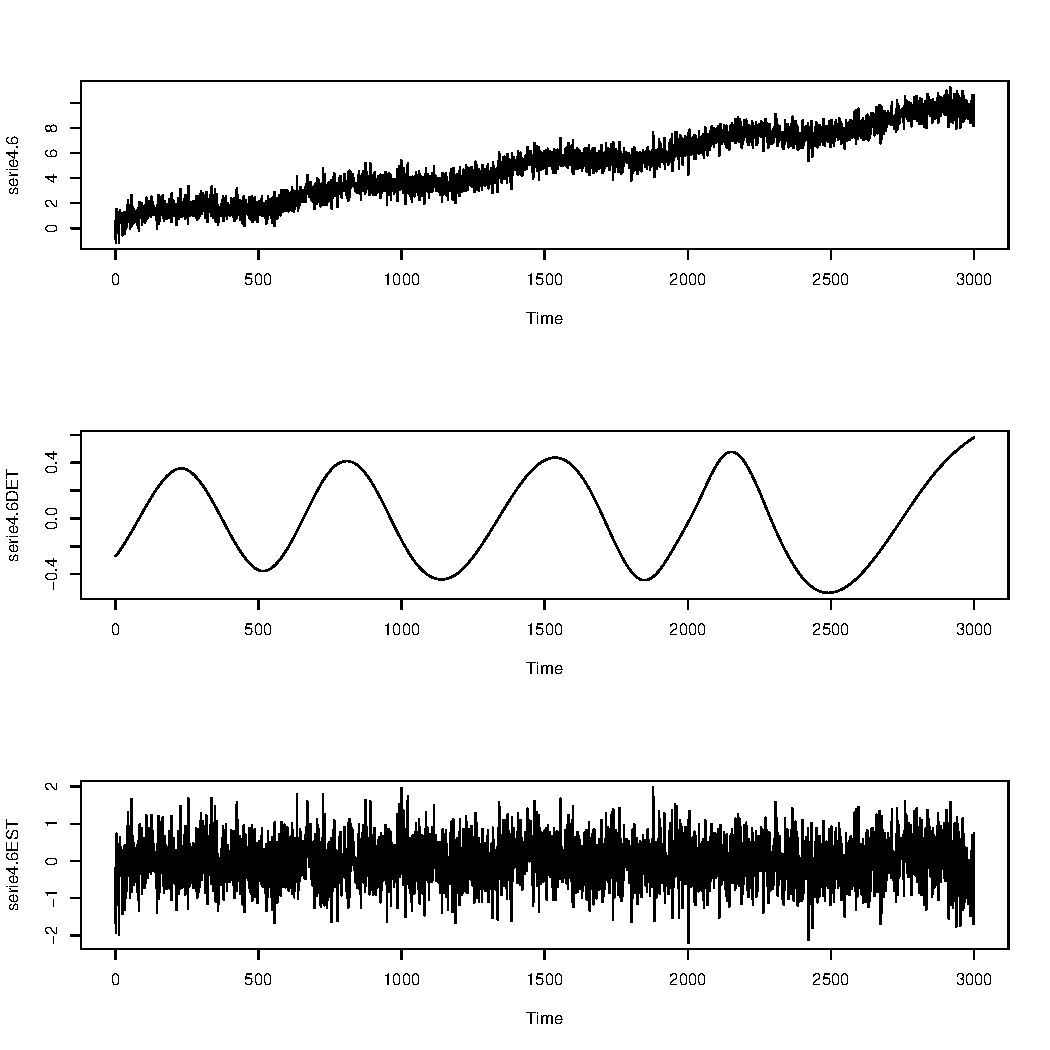
\includegraphics[scale=0.43]{serie4_6.pdf}
 \caption{Série 4.5 e Série 4.6}

\end{center}
\end{figure}

\graphicspath{{imagens/}}
\begin{figure}[H]
\begin{center}
  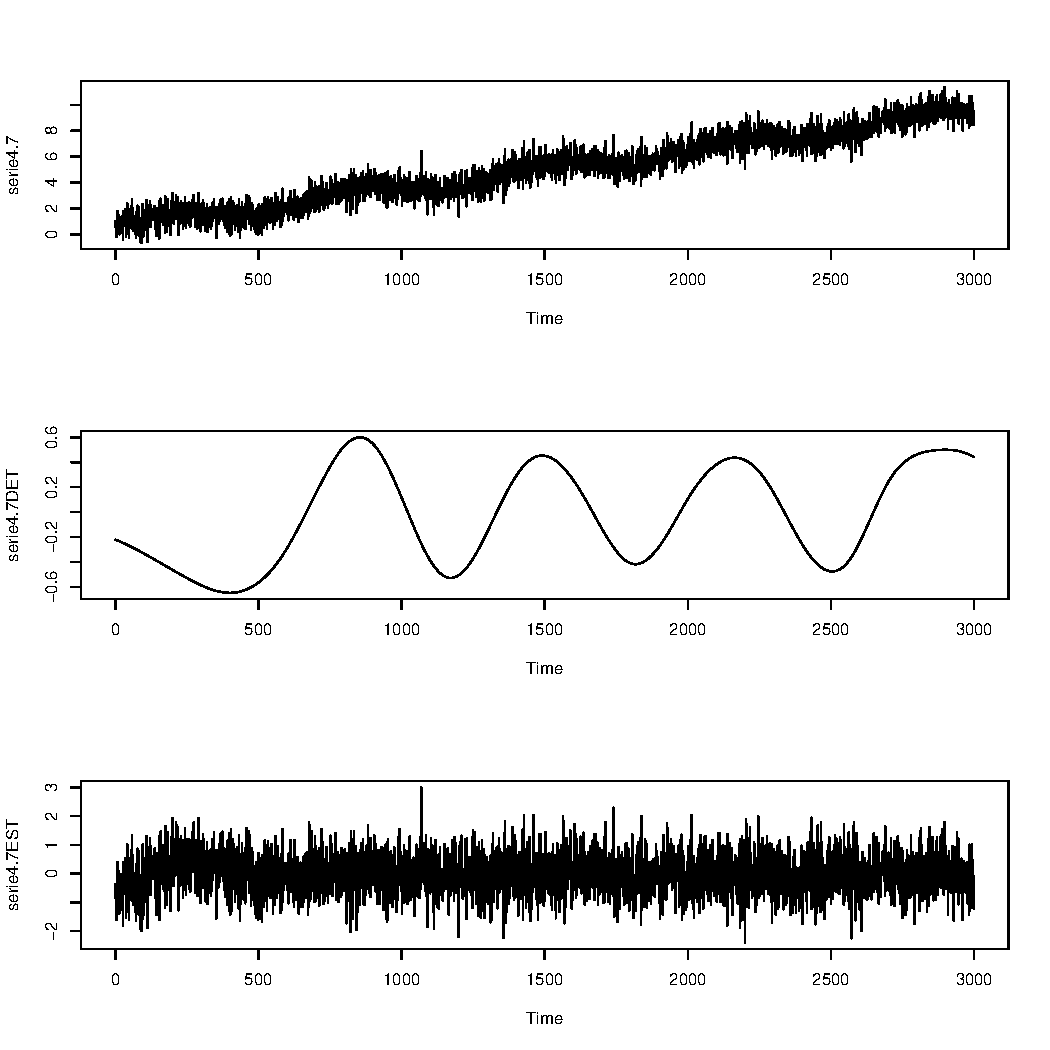
\includegraphics[scale=0.43]{serie4_7.pdf} \quad
  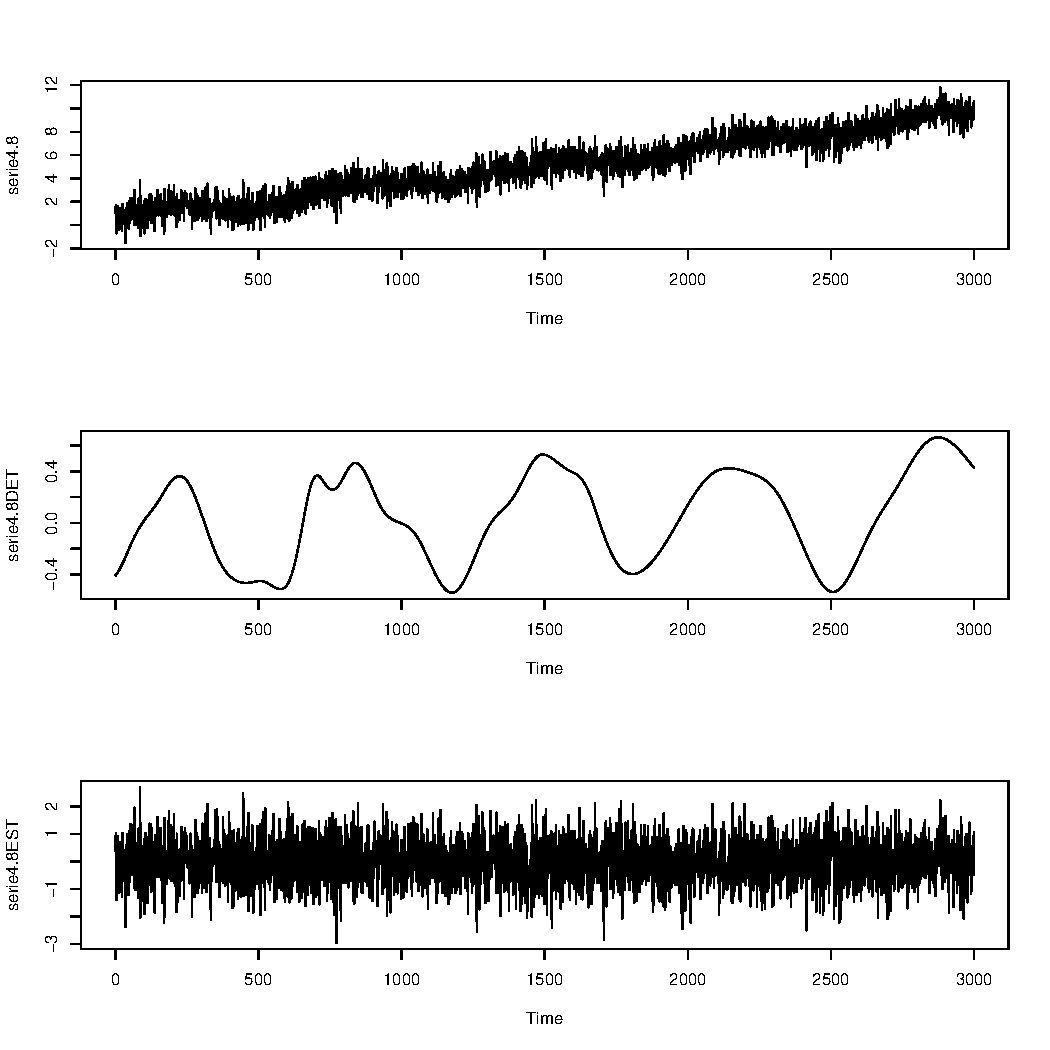
\includegraphics[scale=0.43]{serie4_8.pdf}
  \caption{Série 4.7 e Série 4.8}

\end{center}
\end{figure}

\graphicspath{{imagens/}}
\begin{figure}[H]
\begin{center}
  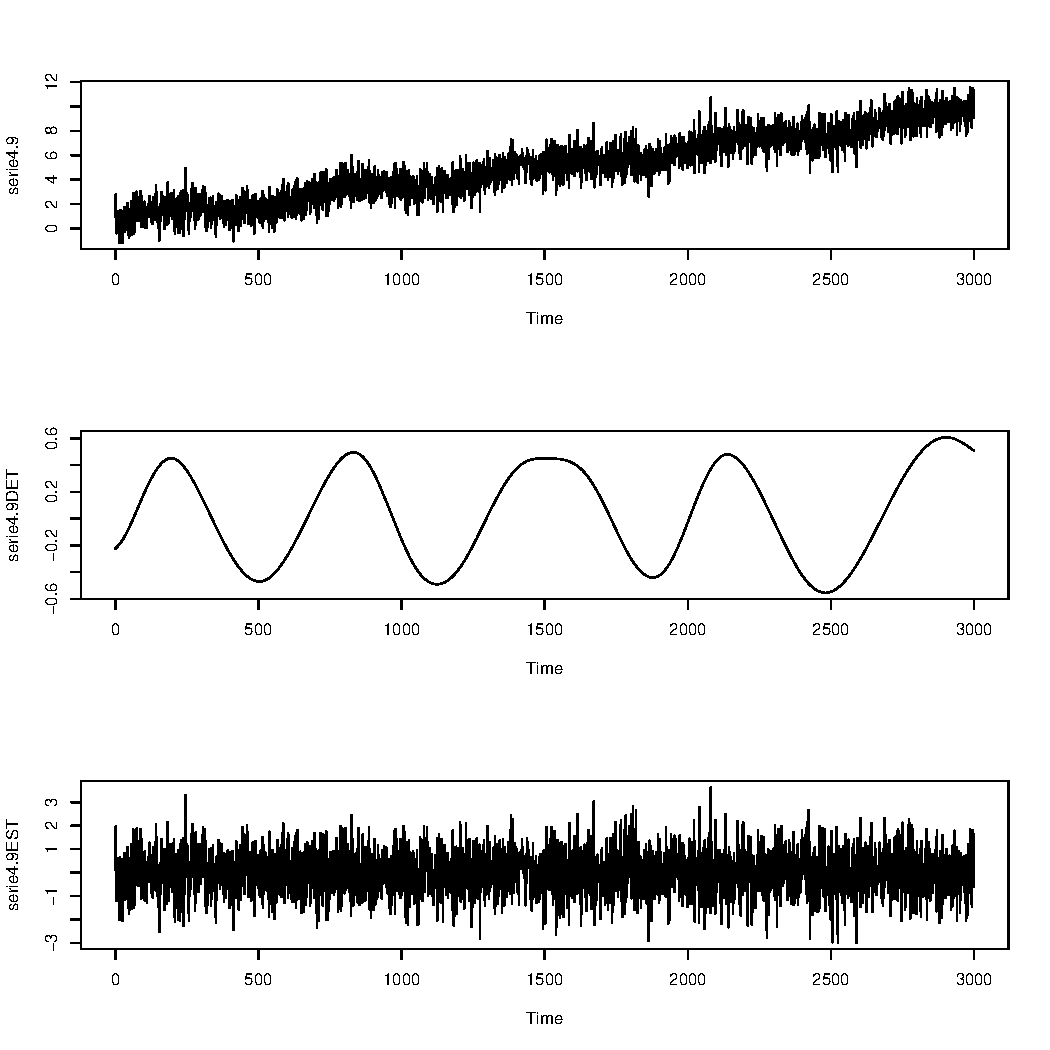
\includegraphics[scale=0.43]{serie4_9.pdf} \quad
  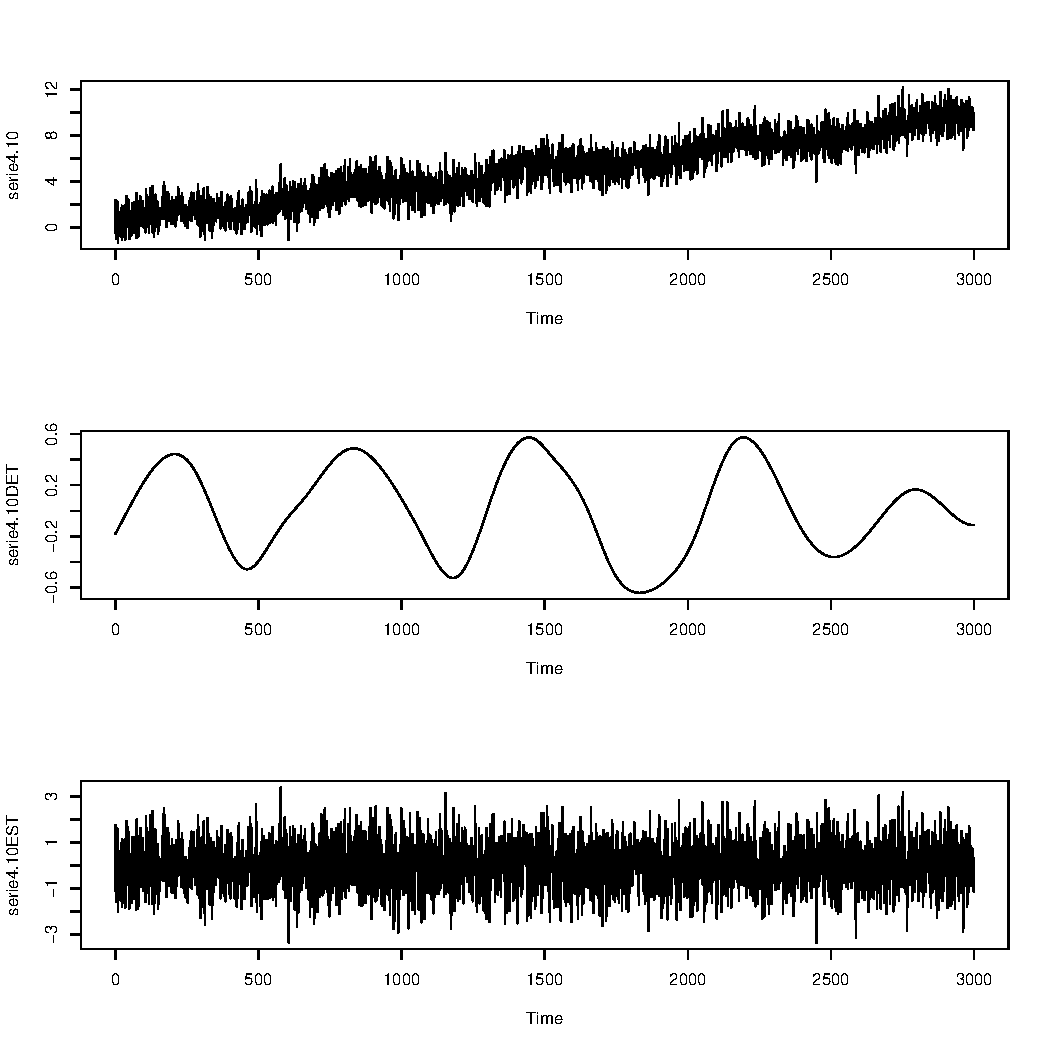
\includegraphics[scale=0.43]{serie4_10.pdf}
  \caption{Série 4.9 e Série 4.10}
\end{center}
\end{figure}
\section{Considerações Finais}
Foram apresentadas as séries temporais utilizadas neste trabalho experimental e suas respactivas decomposições.
% \include{apendice2}
% ...
% \include{apendiceM}

%% Fim do documento
\end{document}
%------------------------------------------------------------------------------------------%
